% generated from JIRA project LVV
% using template at /usr/share/miniconda/envs/docsteady-env/lib/python3.7/site-packages/docsteady/templates/tpr.latex.jinja2.
% using docsteady version 2.1.4
% Please do not edit -- update information in Jira instead
\documentclass[DM,STR,toc]{lsstdoc}
\usepackage{geometry}
\usepackage{longtable,booktabs}
\usepackage{enumitem}
\usepackage{arydshln}
\usepackage{attachfile}
\usepackage{array}
\usepackage{dashrule}

\newcolumntype{L}[1]{>{\raggedright\let\newline\\\arraybackslash\hspace{0pt}}p{#1}}

\input meta.tex

\newcommand{\attachmentsUrl}{https://github.com/\gitorg/\lsstDocType-\lsstDocNum/blob/\gitref/attachments}
\providecommand{\tightlist}{
  \setlength{\itemsep}{0pt}\setlength{\parskip}{0pt}}

\setcounter{tocdepth}{4}

\begin{document}

\def\milestoneName{M2 Functional Re-verification and SAL Interface Verification}
\def\milestoneId{}
\def\product{SIT-COM Integration}

\setDocCompact{true}

\title{LVV-P66: M2 Functional Re-verification and SAL Interface Verification Test Plan and Report}
\setDocRef{\lsstDocType-\lsstDocNum}
\date{ 2021-04-28 }
\author{ Bo Xin }

% Most recent last
\setDocChangeRecord{
\addtohist{}{2021-04-27}{First draft}{Bo Xin}
}

\setDocCurator{Bo Xin}
\setDocUpstreamLocation{\url{https://github.com/lsst-dm/\lsstDocType-\lsstDocNum}}
\setDocUpstreamVersion{\vcsRevision}



\setDocAbstract{
This is the test plan and report for
\textbf{ M2 Functional Re-verification and SAL Interface Verification},
an LSST milestone pertaining to the Data Management Subsystem.\\
This document is based on content automatically extracted from the Jira test database on \docDate.
The most recent change to the document repository was on \vcsDate.
}


\maketitle

\section{Introduction}
\label{sect:intro}


\subsection{Objectives}
\label{sect:objectives}

 {The objective of this test plan is to re-verify the functional
requirements of the M2 Assembly after shipment from the vendor's
facility to the summit facility, as defined in \citeds{LTS-146} and \citeds{LTS-162}. This
test plan consists of two test cycles:~}

\begin{itemize}
\tightlist
\item
  {A preliminary functional test cycle to initially re-verify the M2
  software after delivery to the summit and to prepare for integration
  with the latest version of SAL}
\item
  {A formal test cycle that includes the integration of M2 with the
  latest version of SAL, functional re-verification of the hardware and
  software, and a verification of M2 hazard mitigations.}
\end{itemize}



\subsection{System Overview}
\label{sect:systemoverview}

 {The M2 assembly refers to the secondary mirror (M2 or the surrogate),
the M2 mirror support system, the mirror cell, the mirror cell sensors,
and mirror support control system.}


\subsection{Document Overview}
\label{sect:docoverview}

This document was generated from Jira, obtaining the relevant information from the
\href{https://jira.lsstcorp.org/secure/Tests.jspa\#/testPlan/LVV-P66}{LVV-P66}
~Jira Test Plan and related Test Cycles (
\href{https://jira.lsstcorp.org/secure/Tests.jspa\#/testCycle/LVV-C118}{LVV-C118}
\href{https://jira.lsstcorp.org/secure/Tests.jspa\#/testCycle/LVV-C148}{LVV-C148}
).

Section \ref{sect:intro} provides an overview of the test campaign, the system under test (\product{}),
the applicable documentation, and explains how this document is organized.
Section \ref{sect:testplan} provides additional information about the test plan, like for example the configuration
used for this test or related documentation.
Section \ref{sect:personnel} describes the necessary roles and lists the individuals assigned to them.

Section \ref{sect:overview} provides a summary of the test results, including an overview in Table \ref{table:summary},
an overall assessment statement and suggestions for possible improvements.
Section \ref{sect:detailedtestresults} provides detailed results for each step in each test case.

The current status of test plan \href{https://jira.lsstcorp.org/secure/Tests.jspa\#/testPlan/LVV-P66}{LVV-P66} in Jira is \textbf{ Completed }.

\subsection{References}
\label{sect:references}
\renewcommand{\refname}{}
\bibliography{lsst,refs,books,refs_ads,local}


\newpage
\section{Test Plan Details}
\label{sect:testplan}


\subsection{Data Collection}

  Observing is not required for this test campaign.

\subsection{Verification Environment}
\label{sect:hwconf}
  {The M2 Assembly will be verified on the mirror cart on the 3rd floor of
the Summit Facility.}

  \subsection{Entry Criteria}
  In order to run these tests, the following criteria must be met first:\\

\begin{itemize}
\tightlist
\item
  All utilities and electrical connections are hooked up and allow the
  M2 to be powered on and controlled
\item
  The EFD must be set up to be able to store events and telemetry data
\item
  {Requires the surrogate mirror to be installed in the mirror cell}
\end{itemize}

  \subsection{Exit Criteria}
  In order for this event to be considered complete, the following
criteria must be met:

\begin{itemize}
\tightlist
\item
  Raw test data, events, and telemetry have been saved for M2 in the
  Summit EFD.
\item
  All test data has been analyzed and post processed.
\item
  All test steps have been statused in the Jira Test Cases within this
  Test Plan and actual results populated as required.
\item
  A summary of the results of the test campaign has been captured in the
  Overall Assessment and Recommended Improvements fields of this Test
  Plan
\item
  A link to the verification artifacts used to produce the summary of
  results has been populated in the Verification Artifacts field of this
  Test Plan
\item
  Any failures have been captured in the
  \href{https://jira.lsstcorp.org/projects/FRACAS/issues/}{FRACAS}
  project
\end{itemize}


\subsection{Related Documentation}


No additional documentation provided.


\subsection{PMCS Activity}

Primavera milestones related to the test campaign:
M2 Upgrades Phase 3 -~\url{https://jira.lsstcorp.org/browse/DM-23147}


\newpage
\section{Personnel}
\label{sect:personnel}

The personnel involved in the test campaign is shown in the following table.

{\small
\begin{longtable}{p{3cm}p{3cm}p{3cm}p{6cm}}
\hline
\multicolumn{2}{r}{T. Plan \href{https://jira.lsstcorp.org/secure/Tests.jspa\#/testPlan/LVV-P66}{LVV-P66} owner:} &
\multicolumn{2}{l}{\textbf{ Bo Xin } }\\\hline
\multicolumn{2}{r}{T. Cycle \href{https://jira.lsstcorp.org/secure/Tests.jspa\#/testCycle/LVV-C118}{LVV-C118} owner:} &
\multicolumn{2}{l}{\textbf{
Austin Roberts }
} \\\hline
\textbf{Test Cases} & \textbf{Assigned to} & \textbf{Executed by} & \textbf{Additional Test Personnel} \\ \hline
\href{https://jira.lsstcorp.org/secure/Tests.jspa#/testCase/LVV-T1799}{LVV-T1799}
& {\small Bo Xin } & {\small Bo Xin } &
\begin{minipage}[]{6cm}
\smallskip
{\small {M2 product owner\\
M2 software engineer\\
T\&S Scientist~\\
Electrical support\\
GIS Expert} }
\medskip
\end{minipage}
\\ \hline
\href{https://jira.lsstcorp.org/secure/Tests.jspa#/testCase/LVV-T1798}{LVV-T1798}
& {\small Bo Xin } & {\small Bo Xin } &
\begin{minipage}[]{6cm}
\smallskip
{\small M2 Operator\\
Mechanical Support\\
Electrical Support }
\medskip
\end{minipage}
\\ \hline
\href{https://jira.lsstcorp.org/secure/Tests.jspa#/testCase/LVV-T1827}{LVV-T1827}
& {\small Bo Xin } & {\small Bo Xin } &
\begin{minipage}[]{6cm}
\smallskip
{\small M2 product owner\\
M2 software engineer\\
T\&S Scientist~\\
Electrical support }
\medskip
\end{minipage}
\\ \hline
\href{https://jira.lsstcorp.org/secure/Tests.jspa#/testCase/LVV-T1826}{LVV-T1826}
& {\small Bo Xin } & {\small Bo Xin } &
\begin{minipage}[]{6cm}
\smallskip
{\small M2 product owner\\
M2 software engineer\\
T\&S Scientist~\\
Electrical support }
\medskip
\end{minipage}
\\ \hline
\href{https://jira.lsstcorp.org/secure/Tests.jspa#/testCase/LVV-T1791}{LVV-T1791}
& {\small Bo Xin } & {\small Bo Xin } &
\begin{minipage}[]{6cm}
\smallskip
{\small M2 product owner\\
M2 software engineer\\
T\&S Scientist~\\
Electrical support }
\medskip
\end{minipage}
\\ \hline
\href{https://jira.lsstcorp.org/secure/Tests.jspa#/testCase/LVV-T1829}{LVV-T1829}
& {\small Bo Xin } & {\small  } &
\begin{minipage}[]{6cm}
\smallskip
{\small M2 product owner\\
M2 software engineer\\
T\&S Scientist~\\
Electrical support }
\medskip
\end{minipage}
\\ \hline
\href{https://jira.lsstcorp.org/secure/Tests.jspa#/testCase/LVV-T1810}{LVV-T1810}
& {\small Bo Xin } & {\small Bo Xin } &
\begin{minipage}[]{6cm}
\smallskip
{\small M2 product owner\\
M2 software engineer\\
T\&S Scientist~\\
Electrical support }
\medskip
\end{minipage}
\\ \hline
\href{https://jira.lsstcorp.org/secure/Tests.jspa#/testCase/LVV-T1784}{LVV-T1784}
& {\small Bo Xin } & {\small Bo Xin } &
\begin{minipage}[]{6cm}
\smallskip
{\small M2 product owner\\
M2 software engineer\\
T\&S Scientist~\\
Electrical support }
\medskip
\end{minipage}
\\ \hline
\href{https://jira.lsstcorp.org/secure/Tests.jspa#/testCase/LVV-T1790}{LVV-T1790}
& {\small Bo Xin } & {\small Bo Xin } &
\begin{minipage}[]{6cm}
\smallskip
{\small M2 product owner\\
M2 software engineer\\
T\&S Scientist~\\
Electrical support }
\medskip
\end{minipage}
\\ \hline
\href{https://jira.lsstcorp.org/secure/Tests.jspa#/testCase/LVV-T1788}{LVV-T1788}
& {\small Bo Xin } & {\small Bo Xin } &
\begin{minipage}[]{6cm}
\smallskip
{\small M2 product owner\\
M2 software engineer\\
T\&S Scientist~\\
Electrical support }
\medskip
\end{minipage}
\\ \hline
\href{https://jira.lsstcorp.org/secure/Tests.jspa#/testCase/LVV-T1787}{LVV-T1787}
& {\small Bo Xin } & {\small Bo Xin } &
\begin{minipage}[]{6cm}
\smallskip
{\small M2 product owner\\
M2 software engineer\\
T\&S Scientist~\\
Electrical support }
\medskip
\end{minipage}
\\ \hline
\href{https://jira.lsstcorp.org/secure/Tests.jspa#/testCase/LVV-T1782}{LVV-T1782}
& {\small Bo Xin } & {\small Bo Xin } &
\begin{minipage}[]{6cm}
\smallskip
{\small M2 product owner\\
M2 software engineer\\
T\&S Scientist~\\
Electrical support }
\medskip
\end{minipage}
\\ \hline
\href{https://jira.lsstcorp.org/secure/Tests.jspa#/testCase/LVV-T1792}{LVV-T1792}
& {\small Bo Xin } & {\small Bo Xin } &
\begin{minipage}[]{6cm}
\smallskip
{\small M2 product owner\\
M2 software engineer\\
T\&S Scientist~\\
Electrical support }
\medskip
\end{minipage}
\\ \hline
\href{https://jira.lsstcorp.org/secure/Tests.jspa#/testCase/LVV-T1785}{LVV-T1785}
& {\small Bo Xin } & {\small Bo Xin } &
\begin{minipage}[]{6cm}
\smallskip
{\small M2 product owner\\
M2 software engineer\\
T\&S Scientist~\\
Electrical support }
\medskip
\end{minipage}
\\ \hline
\href{https://jira.lsstcorp.org/secure/Tests.jspa#/testCase/LVV-T1783}{LVV-T1783}
& {\small Bo Xin } & {\small Bo Xin } &
\begin{minipage}[]{6cm}
\smallskip
{\small M2 product owner\\
M2 software engineer\\
T\&S Scientist~\\
Electrical support }
\medskip
\end{minipage}
\\ \hline
\href{https://jira.lsstcorp.org/secure/Tests.jspa#/testCase/LVV-T1786}{LVV-T1786}
& {\small Bo Xin } & {\small Bo Xin } &
\begin{minipage}[]{6cm}
\smallskip
{\small M2 product owner\\
M2 software engineer\\
T\&S Scientist~\\
Electrical support }
\medskip
\end{minipage}
\\ \hline
\href{https://jira.lsstcorp.org/secure/Tests.jspa#/testCase/LVV-T1794}{LVV-T1794}
& {\small Bo Xin } & {\small Bo Xin } &
\begin{minipage}[]{6cm}
\smallskip
{\small M2 product owner\\
M2 software engineer\\
T\&S Scientist~\\
Electrical support }
\medskip
\end{minipage}
\\ \hline
\href{https://jira.lsstcorp.org/secure/Tests.jspa#/testCase/LVV-T1796}{LVV-T1796}
& {\small Bo Xin } & {\small Bo Xin } &
\begin{minipage}[]{6cm}
\smallskip
{\small M2 product owner\\
M2 software engineer\\
T\&S Scientist~\\
Electrical support }
\medskip
\end{minipage}
\\ \hline
\href{https://jira.lsstcorp.org/secure/Tests.jspa#/testCase/LVV-T1795}{LVV-T1795}
& {\small Bo Xin } & {\small Bo Xin } &
\begin{minipage}[]{6cm}
\smallskip
{\small M2 product owner\\
M2 software engineer\\
T\&S Scientist~\\
Electrical support }
\medskip
\end{minipage}
\\ \hline
\href{https://jira.lsstcorp.org/secure/Tests.jspa#/testCase/LVV-T1789}{LVV-T1789}
& {\small Bo Xin } & {\small Bo Xin } &
\begin{minipage}[]{6cm}
\smallskip
{\small M2 product owner\\
M2 software engineer\\
T\&S Scientist~\\
Electrical support }
\medskip
\end{minipage}
\\ \hline
\multicolumn{2}{r}{T. Cycle \href{https://jira.lsstcorp.org/secure/Tests.jspa\#/testCycle/LVV-C148}{LVV-C148} owner:} &
\multicolumn{2}{l}{\textbf{
Austin Roberts }
} \\\hline
\textbf{Test Cases} & \textbf{Assigned to} & \textbf{Executed by} & \textbf{Additional Test Personnel} \\ \hline
\href{https://jira.lsstcorp.org/secure/Tests.jspa#/testCase/LVV-T1803}{LVV-T1803}
& {\small Austin Roberts } & {\small  } &
\begin{minipage}[]{6cm}
\smallskip
{\small Safety Coordinator }
\medskip
\end{minipage}
\\ \hline
\href{https://jira.lsstcorp.org/secure/Tests.jspa#/testCase/LVV-T1614}{LVV-T1614}
& {\small Austin Roberts } & {\small  } &
\begin{minipage}[]{6cm}
\smallskip
{\small (1) Mechanical Engineer\\
(1) Electrical Engineer\\
(1) Software Engineer }
\medskip
\end{minipage}
\\ \hline
\href{https://jira.lsstcorp.org/secure/Tests.jspa#/testCase/LVV-T1613}{LVV-T1613}
& {\small Austin Roberts } & {\small  } &
\begin{minipage}[]{6cm}
\smallskip
{\small (1) Mechanical Engineer\\
(1) Electrical Engineer\\
(1) Software Engineer }
\medskip
\end{minipage}
\\ \hline
\href{https://jira.lsstcorp.org/secure/Tests.jspa#/testCase/LVV-T1615}{LVV-T1615}
& {\small Austin Roberts } & {\small  } &
\begin{minipage}[]{6cm}
\smallskip
{\small (1) Mechanical Engineer\\
(1) Electrical Engineer\\
(1) Software Engineer }
\medskip
\end{minipage}
\\ \hline
\end{longtable}
}

\newpage

\section{Test Campaign Overview}
\label{sect:overview}

\subsection{Summary}
\label{sect:summarytable}

{\small
\begin{longtable}{p{2cm}cp{2.3cm}p{8.6cm}p{2.3cm}}
\toprule
\multicolumn{2}{r}{ T. Plan \href{https://jira.lsstcorp.org/secure/Tests.jspa\#/testPlan/LVV-P66}{LVV-P66}:} &
\multicolumn{2}{p{10.9cm}}{\textbf{ M2 Functional Re-verification and SAL Interface Verification }} & Completed \\\hline
\multicolumn{2}{r}{ T. Cycle \href{https://jira.lsstcorp.org/secure/Tests.jspa\#/testCycle/LVV-C118}{LVV-C118}:} &
\multicolumn{2}{p{10.9cm}}{\textbf{ M2 Preliminary Functional Testing and SAL v4.0 Integration }} & Done \\\hline
\textbf{Test Cases} &  \textbf{Ver.} & \textbf{Status} & \textbf{Comment} & \textbf{Issues} \\\toprule
\href{https://jira.lsstcorp.org/secure/Tests.jspa#/testCase/LVV-T1799}{LVV-T1799}
&  1
& Blocked &
\begin{minipage}[]{9cm}
\smallskip
E-stop did cause loss of power. Test failed because the FAULT state was
not implemented in software.
\medskip
\end{minipage}
&   \href{https://jira.lsstcorp.org/browse/DM-23790}{DM-23790}
\href{https://jira.lsstcorp.org/browse/DM-23790}{DM-23790}
\\\hline
\href{https://jira.lsstcorp.org/secure/Tests.jspa#/testCase/LVV-T1798}{LVV-T1798}
&  1
& Fail &
\begin{minipage}[]{9cm}
\smallskip
Most of the existing telemetry topics passed the test, with one
exception, see LVV-18880. There are quite a few more telemetry topics
that have since been added following the preliminary testing that will
be verified during formal testing.~
\medskip
\end{minipage}
&   \href{https://jira.lsstcorp.org/browse/LVV-18880}{LVV-18880}
\href{https://jira.lsstcorp.org/browse/LVV-18879}{LVV-18879}
\href{https://jira.lsstcorp.org/browse/LVV-18880}{LVV-18880}
\href{https://jira.lsstcorp.org/browse/LVV-18880}{LVV-18880}
\href{https://jira.lsstcorp.org/browse/LVV-18879}{LVV-18879}
\href{https://jira.lsstcorp.org/browse/LVV-18880}{LVV-18880}
\\\hline
\href{https://jira.lsstcorp.org/secure/Tests.jspa#/testCase/LVV-T1827}{LVV-T1827}
&  1
& Pass &
\begin{minipage}[]{9cm}
\smallskip
Inner control loop appears to be working as expected.
\medskip
\end{minipage}
&   \\\hline
\href{https://jira.lsstcorp.org/secure/Tests.jspa#/testCase/LVV-T1826}{LVV-T1826}
&  1
& Pass &
\begin{minipage}[]{9cm}
\smallskip
Both the inner and outer control loops appear to be working properly.
\medskip
\end{minipage}
&   \\\hline
\href{https://jira.lsstcorp.org/secure/Tests.jspa#/testCase/LVV-T1791}{LVV-T1791}
&  1
& Pass &
\begin{minipage}[]{9cm}
\smallskip
Re-positioninig the M2 mirror is shown to be repeatable and the mirror
can stay in position with good stability.
\medskip
\end{minipage}
&   \\\hline
\href{https://jira.lsstcorp.org/secure/Tests.jspa#/testCase/LVV-T1829}{LVV-T1829}
&  2
& Not Executed &
\begin{minipage}[]{9cm}
\smallskip
Not executed because IMS data was only given in the form of 12
displacement sensor readings.~
\medskip
\end{minipage}
&   \href{https://jira.lsstcorp.org/browse/LVV-18872}{LVV-18872}
\href{https://jira.lsstcorp.org/browse/LVV-18872}{LVV-18872}
\\\hline
\href{https://jira.lsstcorp.org/secure/Tests.jspa#/testCase/LVV-T1810}{LVV-T1810}
&  1
& Fail &
\begin{minipage}[]{9cm}
\smallskip
Test failed because the M2 software did not support re-configuration of
the optimal mirror position.
\medskip
\end{minipage}
&   \href{https://jira.lsstcorp.org/browse/LVV-18878}{LVV-18878}
\href{https://jira.lsstcorp.org/browse/LVV-18872}{LVV-18872}
\href{https://jira.lsstcorp.org/browse/LVV-18878}{LVV-18878}
\href{https://jira.lsstcorp.org/browse/LVV-18872}{LVV-18872}
\\\hline
\href{https://jira.lsstcorp.org/secure/Tests.jspa#/testCase/LVV-T1784}{LVV-T1784}
&  1
& Pass &
\begin{minipage}[]{9cm}
\smallskip
After disconnecting power to each actuator {[}B6, C4, D4, A1, A2{]}, we
confirmed that the forces and displacements were maintained.
\medskip
\end{minipage}
&   \\\hline
\href{https://jira.lsstcorp.org/secure/Tests.jspa#/testCase/LVV-T1790}{LVV-T1790}
&  1
& Pass &
\begin{minipage}[]{9cm}
\smallskip
Bump test succeeded without problem.
\medskip
\end{minipage}
&   \\\hline
\href{https://jira.lsstcorp.org/secure/Tests.jspa#/testCase/LVV-T1788}{LVV-T1788}
&  1
& Pass &
\begin{minipage}[]{9cm}
\smallskip
Applied each of the first 20 bending modes in turn. Force accuracy and
repeatability meet requirements.
\medskip
\end{minipage}
&   \\\hline
\href{https://jira.lsstcorp.org/secure/Tests.jspa#/testCase/LVV-T1787}{LVV-T1787}
&  2
& Pass &
\begin{minipage}[]{9cm}
\smallskip
We rotated the M2 cart from 0 to 180 degrees, and verified that the M2
control software applies LUT forces as expected. The M2 inclinometer
works. The reading is used in the LUT. The EUI display of zenith angle
is a mess and needs to be cleaned up.
\medskip
\end{minipage}
&   \\\hline
\href{https://jira.lsstcorp.org/secure/Tests.jspa#/testCase/LVV-T1782}{LVV-T1782}
&  1
& Pass &
\begin{minipage}[]{9cm}
\smallskip
Positions of safety stops were not measured due to lack of hardware
support. Motion limits measured were due to actuator (software) limits.
\medskip
\end{minipage}
&   \href{https://jira.lsstcorp.org/browse/LVV-18874}{LVV-18874}
\href{https://jira.lsstcorp.org/browse/LVV-18874}{LVV-18874}
\\\hline
\href{https://jira.lsstcorp.org/secure/Tests.jspa#/testCase/LVV-T1792}{LVV-T1792}
&  1
& Pass &
\begin{minipage}[]{9cm}
\smallskip
The M2 force balance system appear to work as designed.
\medskip
\end{minipage}
&   \\\hline
\href{https://jira.lsstcorp.org/secure/Tests.jspa#/testCase/LVV-T1785}{LVV-T1785}
&  1
& In Progress &
\begin{minipage}[]{9cm}
\smallskip
We have tested the stiffness of the actuators while they are integrated
with the M2 cell assembly. Standalone (spare) actuators will be needed
to actually reverify this stiffness requirement.
\medskip
\end{minipage}
&   \\\hline
\href{https://jira.lsstcorp.org/secure/Tests.jspa#/testCase/LVV-T1783}{LVV-T1783}
&  1
& Pass &
\begin{minipage}[]{9cm}
\smallskip
Verified that B1 actuator force limit is between 444N and 666N. Did not
have time to test tangent links.
\medskip
\end{minipage}
&   \\\hline
\href{https://jira.lsstcorp.org/secure/Tests.jspa#/testCase/LVV-T1786}{LVV-T1786}
&  1
& Fail &
\begin{minipage}[]{9cm}
\smallskip
We agreed not to re-verify the actuator full stroke using spare
actuators. We will need to locate the software limit switches in the
software, and verify those work properly.
\medskip
\end{minipage}
&   \href{https://jira.lsstcorp.org/browse/LVV-18874}{LVV-18874}
\href{https://jira.lsstcorp.org/browse/LVV-18874}{LVV-18874}
\\\hline
\href{https://jira.lsstcorp.org/secure/Tests.jspa#/testCase/LVV-T1794}{LVV-T1794}
&  1
& Fail &
\begin{minipage}[]{9cm}
\smallskip
Looking at the difference between exhaust and intake temperatures, the
system appear to perform OK in the lab environment.
\medskip
\end{minipage}
&   \href{https://jira.lsstcorp.org/browse/LVV-18863}{LVV-18863}
\href{https://jira.lsstcorp.org/browse/LVV-18875}{LVV-18875}
\href{https://jira.lsstcorp.org/browse/LVV-18863}{LVV-18863}
\href{https://jira.lsstcorp.org/browse/LVV-18875}{LVV-18875}
\\\hline
\href{https://jira.lsstcorp.org/secure/Tests.jspa#/testCase/LVV-T1796}{LVV-T1796}
&  1
& Fail &
\begin{minipage}[]{9cm}
\smallskip
VMS is a separate software CSC, which was not ready at the time of this
testing.
\medskip
\end{minipage}
&   \\\hline
\href{https://jira.lsstcorp.org/secure/Tests.jspa#/testCase/LVV-T1795}{LVV-T1795}
&  2
& Pass &
\begin{minipage}[]{9cm}
\smallskip
The M2 surrogate, together with the mounting pads, weigh about 1590 kg,
which is within the M2 mass budget. Note that this test was not done
with the real M2 glass mirror.
\medskip
\end{minipage}
&   \\\hline
\href{https://jira.lsstcorp.org/secure/Tests.jspa#/testCase/LVV-T1789}{LVV-T1789}
&  1
& Pass &
\begin{minipage}[]{9cm}
\smallskip
The M2 system was shown to work consistently during 4 hours of AOS
operations. The force accuracy and repeatability also appear to meet
requirements. Checked that the M2 control software publishes telemetry
at 20Hz. Also checked that EFD event loss rate and latency are
acceptable.
\medskip
\end{minipage}
&   \\\hline
\multicolumn{2}{r}{ T. Cycle \href{https://jira.lsstcorp.org/secure/Tests.jspa\#/testCycle/LVV-C148}{LVV-C148}:} &
\multicolumn{2}{p{10.9cm}}{\textbf{ M2 Formal Functional Re-Verification and SAL Integration }} & Done \\\hline
\textbf{Test Cases} &  \textbf{Ver.} & \textbf{Status} & \textbf{Comment} & \textbf{Issues} \\\toprule
\href{https://jira.lsstcorp.org/secure/Tests.jspa#/testCase/LVV-T1803}{LVV-T1803}
&  1
& Not Executed &
\begin{minipage}[]{9cm}
\smallskip

\medskip
\end{minipage}
&   \\\hline
\href{https://jira.lsstcorp.org/secure/Tests.jspa#/testCase/LVV-T1614}{LVV-T1614}
&  1
& Not Executed &
\begin{minipage}[]{9cm}
\smallskip

\medskip
\end{minipage}
&   \\\hline
\href{https://jira.lsstcorp.org/secure/Tests.jspa#/testCase/LVV-T1613}{LVV-T1613}
&  1
& Not Executed &
\begin{minipage}[]{9cm}
\smallskip

\medskip
\end{minipage}
&   \\\hline
\href{https://jira.lsstcorp.org/secure/Tests.jspa#/testCase/LVV-T1615}{LVV-T1615}
&  1
& Not Executed &
\begin{minipage}[]{9cm}
\smallskip

\medskip
\end{minipage}
&   \\\hline
\caption{Test Campaign Summary}
\label{table:summary}
\end{longtable}
}

\subsection{Overall Assessment}
\label{sect:overallassessment}

{As a result of the \textbf{preliminary functional test cycle}, the
overall test can be considered a FAIL due to the number of test steps
that failed or were not capable of being executed.~}{However, with each
failed test, we gain a much better understanding of the existing
capabilities of the M2 system, especially with the software. A bug
ticket has been created for each issue that needs to be fixed before the
formal test cycle starts.~}

\subsection{Recommended Improvements}
\label{sect:recommendations}

\textbf{Preliminary Test Cycle}\\
The following are recommended improvements in order to improve the
system as a result of the preliminary functional test cycle:

\begin{itemize}
\tightlist
\item
  Investigate M2 telemetry potential corrupt parameter values
\item
  Fix M2 EUI graphical force distribution
\item
  Enable re-configuring the M2 mirror optimal position (relative to
  mirror cell)
\item
  Enable disabling use of thermal data in M2 LUT (GUI only)
\item
  M2 XML should use TAI instead of UTC
\item
  Clarify the physical locations of M2 temperature sensors
\item
  Locate M2 software limit switches, and fix GUI limit switch panel
\item
  Update M2 GUI display of hardpoint ID numbers
\item
  Add IMS position measurements to M2 SAL and GUI
\item
  Clarify M2 control behavior during slews
\item
  Clean up the M2 zenith angle inconsistency
\item
  Clean up M2 GUI display of the forces
\item
  Display the Fx, Fy, Fz, Mx, My, and Mz that are imposed by the M2
  force balance system
\item
  Add a section to the M2 EUI on the status of the interlock
\item
  Add a GUI command that zero all M2 force offsets
\item
  Add a GUI command to turn on and off the force balance system
\item
  Add telemetry topic PowerStatus
\item
  Define M2 hiTemperatureWarning thresholds
\item
  Make M2 inPoisition threshold configurable
\item
  Implement M2 detailedStates
\item
  Add M2 NetForcesTotal and NetMomentsTotal to GUI and SAL
\end{itemize}

See bug tickets in Jira:
https://jira.lsstcorp.org/issues/?filter=20317\\[2\baselineskip]\textbf{Formal
Test Cycle}\\
The following are recommended improvements in order to improve the
system as a result of the formal functional re-verification test cycle:

\newpage
\section{Detailed Test Results}
\label{sect:detailedtestresults}

\subsection{Test Cycle LVV-C118 }

Open test cycle {\it \href{https://jira.lsstcorp.org/secure/Tests.jspa#/testrun/LVV-C118}{M2 Preliminary Functional Testing and SAL v4.0 Integration}} in Jira.

Test Cycle name: M2 Preliminary Functional Testing and SAL v4.0 Integration\\
Status: Done

The purpose of this preliminary test cycle is to run some basic
functional and software tests to gain an understanding of how the
software performs and what development is required for the CSC to
properly integrate with the latest version of SAL. {The execution of
this test cycle does not require the M2 to be commanded via SAL.~}

\subsubsection{Software Version/Baseline}
\begin{enumerate}
\tightlist
\item
  M2 Control Software with SAL v4.0
\item
  EFD with SAL v4.0
\end{enumerate}

\subsubsection{Configuration}
{No varying configuration between test cycles.}

\subsubsection{Test Cases in LVV-C118 Test Cycle}

\paragraph{ LVV-T1799 - M2 E-stop }\mbox{}\\

Version \textbf{1}.
Open  \href{https://jira.lsstcorp.org/secure/Tests.jspa#/testCase/LVV-T1799}{\textit{ LVV-T1799 } }
test case in Jira.

{The purpose of this test case is to re-verify the M2 interlocks
requirement, as defined in \citeds{LTS-146}, after shipment from the vendor's
facility to the Summit facility. The results of this test should show
that the M2 support control system behaves as expected, sending the
system into a FAULT state when the E-stop is pressed and cutting all
power from the M2 actuators. This test case will only exercise this
functionality and meets the following criteria:}\\

\begin{itemize}
\tightlist
\item
  Only requires the use of an E-stop in place of the interlock system
\item
  Only requires the current version of SAL
\item
  Only requires the surrogate mirror to be installed
\end{itemize}

\textbf{ Preconditions}:\\
{Prior to the execution of this test case to re-verify the M2 E-stop
functionality, the following Summit tasks must be completed:}

\begin{itemize}
\tightlist
\item
  {Replace relay in M2 Pilz interlock and install E-Stop}

  \begin{itemize}
  \tightlist
  \item
    {\url{https://jira.lsstcorp.org/browse/SUMMIT-3927}}{\\
    }
  \end{itemize}
\end{itemize}

Execution status: {\bf Blocked }

Final comment:\\E-stop did cause loss of power. Test failed because the FAULT state was
not implemented in software.

Issues found during the execution of LVV-T1799 test case:

\begin{itemize}
\item \href{https://jira.lsstcorp.org/browse/DM-23790}{DM-23790}~~Support the Fault State

\end{itemize}

Detailed steps results:

\begin{tabular}{p{2cm}p{14cm}}
\toprule
Step 1 & Step Execution Status: \textbf{ Pass } \\ \hline
\end{tabular}
 Description \\
{\footnotesize
Power up the M2 control system and enter closed loop mode.

}
\hdashrule[0.5ex]{\textwidth}{1pt}{3mm}
  Expected Result \\
{\footnotesize
The M2 control system enters closed loop mode.

}
\hdashrule[0.5ex]{\textwidth}{1pt}{3mm}
  Actual Result \\
{\footnotesize
12:04pm local. 3/3/2020\\
enter close loop mode\\
hit e stop\\
GUI shows ``alarm active'' in red

}
\begin{tabular}{p{2cm}p{14cm}}
\toprule
Step 2 & Step Execution Status: \textbf{ Fail } \\ \hline
\end{tabular}
 Description \\
{\footnotesize
Press E-stop

}
\hdashrule[0.5ex]{\textwidth}{1pt}{3mm}
  Expected Result \\
{\footnotesize
The M2 transitions into fault state.

}
\hdashrule[0.5ex]{\textwidth}{1pt}{3mm}
  Actual Result \\
{\footnotesize
No Fault State has been implemented in the software. Te-wei will fix
this after initial round of testing.

}
\hdashrule[0.5ex]{\textwidth}{1pt}{3mm}
  Issues found executing this step:  \\
{\footnotesize
\begin{itemize}
\item \href{https://jira.lsstcorp.org/browse/DM-23790}{DM-23790}~~Support the Fault State

\end{itemize}
}
\begin{tabular}{p{2cm}p{14cm}}
\toprule
Step 3 & Step Execution Status: \textbf{ Pass } \\ \hline
\end{tabular}
 Description \\
{\footnotesize
recover the system:

\begin{itemize}
\tightlist
\item
  switch e-stop off then back on
\item
  observe system behaviors:alarms, warnings
\item
  clear the errors
\item
  reenter local mode, then diagnostic mode, then enable closed loop
\end{itemize}

}
\hdashrule[0.5ex]{\textwidth}{1pt}{3mm}
  Expected Result \\
{\footnotesize
The system is able to be transitioned out of the Fault state

}
\hdashrule[0.5ex]{\textwidth}{1pt}{3mm}
  Actual Result \\
{\footnotesize
e-stop switch -\textgreater{} off, then on\\
in GUI, click ``alarms/warnings'' , then ``reset all items''\\
in mode control (GUI), go to Remote mode (known bug, according to
Te-Wei, otherwise it will all crash)\\
Quit the GUI\\
12:11pm\\
copied over the binary files\\
restart the system, by clicking on a small arrow on the upper left of
GUI\\
in the GUI message window, confirm ``SAL interface has started''\\
check the terminal window, confirm things are ready.\\
Mode control -\textgreater{} local\\
local mode -\textgreater{} diagnostic -\textgreater{} enable\\
12:31pm, some alarms showed up, including ILC read error. power relay
open fault.\\
reset all items, enable, still error\\
Got Franco here. We need to push and RELEASE (by twisting slightly) the
e-stop. 12:38pm. Franco did this, and we reset all items, enable. All
seems good now.\\
To shut down, open loop, stand by, remote, quit~

}

\paragraph{ LVV-T1798 - verify M2 SAL4.0 telemetry against EUI display and output binary files }\mbox{}\\

Version \textbf{1}.
Open  \href{https://jira.lsstcorp.org/secure/Tests.jspa#/testCase/LVV-T1798}{\textit{ LVV-T1798 } }
test case in Jira.

The objective of this test case is to verify the M2's ability to
accurately publish telemetry as specified in \citeds{LTS-146} and \citeds{LTS-162}. In
order to do so, the telemetry data being published to the EFD must first
be compared to the information that is displayed on the EUI and on an
output binary file from Matlab. Once the initial telemetry data is seen
to be consistent across the EFD, the EUI and the output binary file, 20N
of force will be loaded onto one of the actuators. The purpose of this
will be to verify that the telemetry data accurately reports the 20N of
added force. If the telemetry is confirmed to be accurate, we will
verify that the telemetry topics specified in \citeds{LTS-162} are all
consistently reported through the EFD, EUI and output binary files. This
test case will exercise this functionality and meets the following
criteria:

\begin{itemize}
\tightlist
\item
  Only requires the most current version of SAL
\item
  Only requires the surrogate mirror to be installed
\item
  Only requires commands to be sent through the CSC
\item
  Only requires a python notebook to read output binary file
\item
  Does require telemetry data to be recorded from the EUI, EFD and an
  output binary file
\end{itemize}

\textbf{ Preconditions}:\\
{Prior to the execution of this test case to re-verify the M2 SAL 4.0
telemetry and events, the following Summit tasks must be completed:}

\begin{itemize}
\tightlist
\item
  {Verify M2 SAL functionality/update to latest version of SAL}

  \begin{itemize}
  \tightlist
  \item
    {\url{https://jira.lsstcorp.org/browse/SUMMIT-863}}
  \end{itemize}
\item
  {Check on the M2 surrogate AO control}

  \begin{itemize}
  \tightlist
  \item
    {\url{https://jira.lsstcorp.org/browse/SUMMIT-3518}}
  \end{itemize}
\end{itemize}

Execution status: {\bf Fail }

Final comment:\\Most of the existing telemetry topics passed the test, with one
exception, see LVV-18880. There are quite a few more telemetry topics
that have since been added following the preliminary testing that will
be verified during formal testing.~

Issues found during the execution of LVV-T1798 test case:

\begin{itemize}
\item \href{https://jira.lsstcorp.org/browse/LVV-18880}{LVV-18880}~~Investigate M2 telemetry potential corrupt parameter values

\item \href{https://jira.lsstcorp.org/browse/LVV-18879}{LVV-18879}~~Fix M2 EUI graphical force distribution

\item \href{https://jira.lsstcorp.org/browse/LVV-18880}{LVV-18880}~~Investigate M2 telemetry potential corrupt parameter values

\end{itemize}

Detailed steps results:

\begin{tabular}{p{2cm}p{14cm}}
\toprule
Step 1 & Step Execution Status: \textbf{ Pass } \\ \hline
\end{tabular}
 Description \\
{\footnotesize
Power up\textbf{~}the control system and observe the current information
in the EUI

}
\hdashrule[0.5ex]{\textwidth}{1pt}{3mm}
  Expected Result \\
{\footnotesize
The telemetry and events are published to the EFD and are consistent to
the information displayed on the EUI.

}
\hdashrule[0.5ex]{\textwidth}{1pt}{3mm}
  Actual Result \\
{\footnotesize
1:50pm local started.\\
Seems like the ``force error'' displayed in GUI has nothing to do with
close loop vs open loop. Most likely it is applied forces vs measured
forces.\\
According to Te-Wei, these are the available topics in EFD:\\
mirrorPositionMeasured: in GUI, go to rigid body position, right column,
they match EFD. GUI unit: mm, urad, EFD unit: um, rad\\
axialForcesMeasured: this telemetry seems to match F\_CUR in the GUI
(CUR for current). We switched between open and close loop a few times,
nothing seem to change on the GUI nor EFD. time is 3:12pm now.\\
tangentForcesMeasured: checked GUI against EFD, they match\\
temperaturesMeasured: GUI -\textgreater{} utility view show 16
temperature measurements. there are 72 fields, but only 16 sensors. Need
to do LCR to change XML and sal\_interface document. For now, we use
-999 for non-existent sensors. Otherwise there is NaN the entire topic
is dropped by Kafka producer. Angelo will fix this, but for now, Bo
decided to use -999, so that data can go into EFD which facilitates
subsequent analysis. The 12 mirror sensors on the GUI should correspond
to fields temp0-11. Randomly checked 2 out of the 12, seem to match.\\
zenithAngleMeasured: two places in GUI (utility view vs cell status)
show 89.50 and 89.57. EFD shows 7.4e-3, unit is radian.\\
axialActuatorAbsolutePositionSteps: compare this to GUI. when entering
closed loop, these get updated (with T and Angle), observed the change
in EFD is same as change in GUI. So somehow they have different
offsets.\\
tangentActuatorAbsolutePositionSteps: same as above. different offset,
but change by the same amount.\\
axialActuatorPositionAbsoluteEncoderPositionMeasured: correspond to
GUI-\textgreater{}Positon-\textgreater{}mm. But unit is um in EFD\\
tangentActuatorPositionAbsoluteEncoderPositionMeasured: same as above\\
check events now:\\
summaryState: yes, diagnostic = 1, enable =2, standby=5; what Harris
calls diagnostic mode is what we call disabled mode. Other than that,
current events do not have detailed state, like open loop vs closed
loop. That is all the issues we have on the states. Te-Wei confirms
that.\\
m2AssemblyInPosition: inPosition box lights up when a log event is sent.
The logevent is published at the close loop update rate. IN open loop,
it seems to still publish these log events. Te-Wei says it is due to the
bug (error as seen in message window: E6052 monitoring ILC read error)\\
SELECT inPosition AS ``mean\_inPosition'' FROM
``efd''.``autogen''.``lsst.sal.MTM2.logevent\_m2AssemblyInPosition''
WHERE time \textgreater{} :dashboardTime: FILL(null)\\
errorCode: EFD shows many 6052 and 0s, consistent with GUI message
window (it is a bug, btw). 0 error code doesn't show in GUI window.\\
appliedSettingsMatchStart: this shows settings are read and applied.
This only happens when we quite the GUI, then restart, check 18:20utc.
According to Te-Wei, this is triggered by transitioning into enabled
state from diagnostic/disable

}
\begin{tabular}{p{2cm}p{14cm}}
\toprule
Step 2 & Step Execution Status: \textbf{ Pass } \\ \hline
\end{tabular}
 Description \\
{\footnotesize
In closed loop mode, add 20N to actuator B1.

}
\hdashrule[0.5ex]{\textwidth}{1pt}{3mm}
  Expected Result \\
{\footnotesize
In the EUI, the F\_cur field of actuator B1 shows 20N of added force
after the command has been given.

}
\hdashrule[0.5ex]{\textwidth}{1pt}{3mm}
  Actual Result \\
{\footnotesize
5:20pm local\\
enter closed loop, so that we can load forces. (Te-Wei is sure that in
the open loop mode we can only load steps)\\
Bo created add20N.csv, Te-Wei converted into add20N.scp\\
we loaded with GUI, confirmed force (F\_CUR in GUI) increase from
\textasciitilde{}185 N to \textasciitilde{}205N. observed this force
change in EFD, 21:49 utc\\
Te-Wei recommended that we not to shut down the control system at the
end of each test case, because there are always issues when we restart
it. The memory has to be cleared with a script. And we see errors and
typically have to retry a few times.\\
We did not need to make another csv with -20N on B1. We went to open
loop, then came back to closed loop, so that the forces are recalculated
based on LUT.

}
\begin{tabular}{p{2cm}p{14cm}}
\toprule
Step 3 & Step Execution Status: \textbf{ Fail } \\ \hline
\end{tabular}
 Description \\
{\footnotesize
Perform data analysis:

\begin{itemize}
\tightlist
\item
  compare the output binary file to SAL events \& telemetry from EFD
\item
  Check all the events \& telemetry info available, including, e.g. VMS,
  temperature, position sensors, etc.
\item
  In the same notebook, we query EFD and compare
\end{itemize}

}
\hdashrule[0.5ex]{\textwidth}{1pt}{3mm}
  Test Data \\
 {\footnotesize
Note: use Harris readLabViewBinary.m to read in data from binary, then
save as Matlab mat file. Python notebook can read Matlab lab mat file.

}
\hdashrule[0.5ex]{\textwidth}{1pt}{3mm}
  Expected Result \\
{\footnotesize
The telemetry data published to the EFD is consistent to data on both
the output binary file and the EUI.

}
\hdashrule[0.5ex]{\textwidth}{1pt}{3mm}
  Actual Result \\
{\footnotesize
All telemetry are checked:\\
\href{https://github.com/bxin/M2_summit_2003/blob/master/a02_check_telemetry.ipynb}{a02\_check\_telemetry.ipynb}\\
all log events are checked:\\
\href{https://github.com/bxin/M2_summit_2003/blob/master/a07_log_events.ipynb}{a07\_log\_events.ipynb}\\
Note:current architecture requires VMS to be part of a separate CSC,
together with VMS for M1M3 and TMA. So there is no VMS telemetry in M2
XML.

}
\hdashrule[0.5ex]{\textwidth}{1pt}{3mm}
  Issues found executing this step:  \\
{\footnotesize
\begin{itemize}
\item \href{https://jira.lsstcorp.org/browse/LVV-18880}{LVV-18880}~~Investigate M2 telemetry potential corrupt parameter values

\end{itemize}
}
\begin{tabular}{p{2cm}p{14cm}}
\toprule
Step 4 & Step Execution Status: \textbf{ Pass } \\ \hline
\end{tabular}
 Description \\
{\footnotesize
Check the MirrorPositionMeasured (MTM2\_position) topic published to the
EFD.

}
\hdashrule[0.5ex]{\textwidth}{1pt}{3mm}
  Expected Result \\
{\footnotesize
The data is consistent to what is on the EUI display and output binary
file.

}
\hdashrule[0.5ex]{\textwidth}{1pt}{3mm}
  Actual Result \\
{\footnotesize

}
\begin{tabular}{p{2cm}p{14cm}}
\toprule
Step 5 & Step Execution Status: \textbf{ Blocked } \\ \hline
\end{tabular}
 Description \\
{\footnotesize
Check the AxialForceData (MTM2\_axialForce) topic published to the EFD.

}
\hdashrule[0.5ex]{\textwidth}{1pt}{3mm}
  Expected Result \\
{\footnotesize
The data is consistent to what is on the EUI display and output binary
file.

}
\hdashrule[0.5ex]{\textwidth}{1pt}{3mm}
  Actual Result \\
{\footnotesize

}
\hdashrule[0.5ex]{\textwidth}{1pt}{3mm}
  Issues found executing this step:  \\
{\footnotesize
\begin{itemize}
\item \href{https://jira.lsstcorp.org/browse/LVV-18879}{LVV-18879}~~Fix M2 EUI graphical force distribution

\end{itemize}
}
\begin{tabular}{p{2cm}p{14cm}}
\toprule
Step 6 & Step Execution Status: \textbf{ Pass } \\ \hline
\end{tabular}
 Description \\
{\footnotesize
Check the TangentForceData (MTM2\_tangentForce) topic published to the
EFD.

}
\hdashrule[0.5ex]{\textwidth}{1pt}{3mm}
  Expected Result \\
{\footnotesize
The data is consistent to what is on the EUI display and output binary
file.

}
\hdashrule[0.5ex]{\textwidth}{1pt}{3mm}
  Actual Result \\
{\footnotesize

}
\begin{tabular}{p{2cm}p{14cm}}
\toprule
Step 7 & Step Execution Status: \textbf{ Not Executed } \\ \hline
\end{tabular}
 Description \\
{\footnotesize
Check the BalanceForceData (MTM2\_forceBalance) topic published to the
EFD.

}
\hdashrule[0.5ex]{\textwidth}{1pt}{3mm}
  Expected Result \\
{\footnotesize
The data is consistent to what is on the EUI display and output binary
file.

}
\hdashrule[0.5ex]{\textwidth}{1pt}{3mm}
  Actual Result \\
{\footnotesize

}
\begin{tabular}{p{2cm}p{14cm}}
\toprule
Step 8 & Step Execution Status: \textbf{ Not Executed } \\ \hline
\end{tabular}
 Description \\
{\footnotesize
Check the NetForcesTotal (MTM2\_netForcesTotal) topic published to the
EFD.

}
\hdashrule[0.5ex]{\textwidth}{1pt}{3mm}
  Expected Result \\
{\footnotesize
The data is consistent to what is on the EUI display and output binary
file.

}
\hdashrule[0.5ex]{\textwidth}{1pt}{3mm}
  Actual Result \\
{\footnotesize

}
\begin{tabular}{p{2cm}p{14cm}}
\toprule
Step 9 & Step Execution Status: \textbf{ Not Executed } \\ \hline
\end{tabular}
 Description \\
{\footnotesize
Check the NetMomentsTotal (MTM2\_netMomentsTotal) topic published to the
EFD.

}
\hdashrule[0.5ex]{\textwidth}{1pt}{3mm}
  Expected Result \\
{\footnotesize
The data is consistent to what is on the EUI display and output binary
file.

}
\hdashrule[0.5ex]{\textwidth}{1pt}{3mm}
  Actual Result \\
{\footnotesize

}
\begin{tabular}{p{2cm}p{14cm}}
\toprule
Step 10 & Step Execution Status: \textbf{ Pass } \\ \hline
\end{tabular}
 Description \\
{\footnotesize
Check the TemperaturesMeasured (MTM2\_temperature) topic published to
the EFD.

}
\hdashrule[0.5ex]{\textwidth}{1pt}{3mm}
  Expected Result \\
{\footnotesize
The data is consistent to what is on the EUI display and output binary
file.

}
\hdashrule[0.5ex]{\textwidth}{1pt}{3mm}
  Actual Result \\
{\footnotesize

}
\begin{tabular}{p{2cm}p{14cm}}
\toprule
Step 11 & Step Execution Status: \textbf{ Not Executed } \\ \hline
\end{tabular}
 Description \\
{\footnotesize
Check the ZenithAngleData (MTM2\_zenithAngle) topic published to the
EFD.

}
\hdashrule[0.5ex]{\textwidth}{1pt}{3mm}
  Expected Result \\
{\footnotesize
The data is consistent to what is on the EUI display and output binary
file and the units are degrees.

}
\hdashrule[0.5ex]{\textwidth}{1pt}{3mm}
  Actual Result \\
{\footnotesize

}
\begin{tabular}{p{2cm}p{14cm}}
\toprule
Step 12 & Step Execution Status: \textbf{ Pass } \\ \hline
\end{tabular}
 Description \\
{\footnotesize
Check the AxialActuatorSteps (MTM2\_axialAcutatorSteps) topic published
to the EFD.

}
\hdashrule[0.5ex]{\textwidth}{1pt}{3mm}
  Expected Result \\
{\footnotesize
The data is consistent to what is on the EUI display and output binary
file.

}
\hdashrule[0.5ex]{\textwidth}{1pt}{3mm}
  Actual Result \\
{\footnotesize

}
\begin{tabular}{p{2cm}p{14cm}}
\toprule
Step 13 & Step Execution Status: \textbf{ Not Executed } \\ \hline
\end{tabular}
 Description \\
{\footnotesize
Check the MTM2\_tangentActuatorSteps topic published to the EFD

}
\hdashrule[0.5ex]{\textwidth}{1pt}{3mm}
  Expected Result \\
{\footnotesize
The data is consistent to what is on the EUI display and output binary
file.

}
\hdashrule[0.5ex]{\textwidth}{1pt}{3mm}
  Actual Result \\
{\footnotesize

}
\begin{tabular}{p{2cm}p{14cm}}
\toprule
Step 14 & Step Execution Status: \textbf{ Not Executed } \\ \hline
\end{tabular}
 Description \\
{\footnotesize
Check the axialEncoderPositions topic published to the EFD.

}
\hdashrule[0.5ex]{\textwidth}{1pt}{3mm}
  Expected Result \\
{\footnotesize
The data is consistent to what is on the EUI display and output binary
file.

}
\hdashrule[0.5ex]{\textwidth}{1pt}{3mm}
  Actual Result \\
{\footnotesize

}
\begin{tabular}{p{2cm}p{14cm}}
\toprule
Step 15 & Step Execution Status: \textbf{ Fail } \\ \hline
\end{tabular}
 Description \\
{\footnotesize
Check the TangentEncoderPositions (MTM2\_tangentEncoderSteps) topic
published to the EFD.

}
\hdashrule[0.5ex]{\textwidth}{1pt}{3mm}
  Expected Result \\
{\footnotesize
The data is consistent to what is on the EUI display and output binary
file.

}
\hdashrule[0.5ex]{\textwidth}{1pt}{3mm}
  Actual Result \\
{\footnotesize

}
\hdashrule[0.5ex]{\textwidth}{1pt}{3mm}
  Issues found executing this step:  \\
{\footnotesize
\begin{itemize}
\item \href{https://jira.lsstcorp.org/browse/LVV-18880}{LVV-18880}~~Investigate M2 telemetry potential corrupt parameter values

\end{itemize}
}
\begin{tabular}{p{2cm}p{14cm}}
\toprule
Step 16 & Step Execution Status: \textbf{ Not Executed } \\ \hline
\end{tabular}
 Description \\
{\footnotesize
Check the ILCData ({MTM2\_ilcData)} topic published to the EFD.

}
\hdashrule[0.5ex]{\textwidth}{1pt}{3mm}
  Expected Result \\
{\footnotesize
The data is consistent to what is on the EUI display and output binary
file.

}
\hdashrule[0.5ex]{\textwidth}{1pt}{3mm}
  Actual Result \\
{\footnotesize

}
\begin{tabular}{p{2cm}p{14cm}}
\toprule
Step 17 & Step Execution Status: \textbf{ Not Executed } \\ \hline
\end{tabular}
 Description \\
{\footnotesize
Check the PowerStatus (MTM2\_powerStatus) topic published to the EFD.

}
\hdashrule[0.5ex]{\textwidth}{1pt}{3mm}
  Expected Result \\
{\footnotesize
The data is consistent to what is on the EUI display and output binary
file.

}
\hdashrule[0.5ex]{\textwidth}{1pt}{3mm}
  Actual Result \\
{\footnotesize

}
\begin{tabular}{p{2cm}p{14cm}}
\toprule
Step 18 & Step Execution Status: \textbf{ Not Executed } \\ \hline
\end{tabular}
 Description \\
{\footnotesize
Check the DisplacementSensors ({MTM2\_displacementSensors)} topic
published to the EFD.

}
\hdashrule[0.5ex]{\textwidth}{1pt}{3mm}
  Expected Result \\
{\footnotesize
The data is consistent to what is on the EUI display and output binary
file.

}
\hdashrule[0.5ex]{\textwidth}{1pt}{3mm}
  Actual Result \\
{\footnotesize

}
\begin{tabular}{p{2cm}p{14cm}}
\toprule
Step 19 & Step Execution Status: \textbf{ Not Executed } \\ \hline
\end{tabular}
 Description \\
{\footnotesize
Check the MirrorPositionMeasuredIMS (MTM2\_positionIMS) topic published
to the EFD.

}
\hdashrule[0.5ex]{\textwidth}{1pt}{3mm}
  Expected Result \\
{\footnotesize
The data is consistent to what is on the EUI display and output binary
file.

}
\hdashrule[0.5ex]{\textwidth}{1pt}{3mm}
  Actual Result \\
{\footnotesize

}
\begin{tabular}{p{2cm}p{14cm}}
\toprule
Step 20 & Step Execution Status: \textbf{ Not Executed } \\ \hline
\end{tabular}
 Description \\
{\footnotesize
Check that the GUI has been updated to match the categorization of the
forces in the SAL telemetry

}
\hdashrule[0.5ex]{\textwidth}{1pt}{3mm}
  Expected Result \\
{\footnotesize
The GUI should include the total forces, measured forces, LUT\_gravity
forces, LUT\_thermal forces, user\_applied forces (including AOS
forces), and balance forces

}
\hdashrule[0.5ex]{\textwidth}{1pt}{3mm}
  Actual Result \\
{\footnotesize

}

\paragraph{ LVV-T1827 - M2 inner loop control - open loop mode }\mbox{}\\

Version \textbf{1}.
Open  \href{https://jira.lsstcorp.org/secure/Tests.jspa#/testCase/LVV-T1827}{\textit{ LVV-T1827 } }
test case in Jira.

{The purpose of this test case is to re-verify the inner control loop
requirement, as specified in \citeds{LTS-146}, after shipment from the vendor's
facility to the Summit facility. This test is meant to show that the
inner control loop applies motor steps as commanded in open loop mode.
This test case will exercise this functionality and meets the following
criteria:}

\begin{itemize}
\tightlist
\item
  Only requires the most current version of SAL
\item
  Only requires the surrogate mirror to be installed
\item
  Only requires the M2 to be operated in open loop mode
\item
  Does require telemetry data to be recorded from the EUI, EFD and an
  output binary file
\end{itemize}

\textbf{ Preconditions}:\\


Execution status: {\bf Pass }

Final comment:\\Inner control loop appears to be working as expected.


Detailed steps results:

\begin{tabular}{p{2cm}p{14cm}}
\toprule
Step 1 & Step Execution Status: \textbf{ Pass } \\ \hline
\end{tabular}
 Description \\
{\footnotesize
With the M2 surrogate facing down, power up the M2 control system and
enter open-loop mode

}
\hdashrule[0.5ex]{\textwidth}{1pt}{3mm}
  Expected Result \\
{\footnotesize
The M2 control system is able to enter open-loop mode.

}
\hdashrule[0.5ex]{\textwidth}{1pt}{3mm}
  Actual Result \\
{\footnotesize

}
\begin{tabular}{p{2cm}p{14cm}}
\toprule
Step 2 & Step Execution Status: \textbf{ Pass } \\ \hline
\end{tabular}
 Description \\
{\footnotesize
For the following steps, write down the following information from the
EUI:

\begin{itemize}
\tightlist
\item
  B1 position
\item
  steps
\item
  e\_count
\item
  F\_cmd
\item
  F\_cur
\item
  F\_HC
\item
  F\_error
\end{itemize}

}
\hdashrule[0.5ex]{\textwidth}{1pt}{3mm}
  Expected Result \\
{\footnotesize
The EUI displays telemetry data for the following categories.

}
\hdashrule[0.5ex]{\textwidth}{1pt}{3mm}
  Actual Result \\
{\footnotesize
\href{https://github.com/bxin/M2_summit_2003/blob/master/M2basicTest.xlsx}{M2basicTest.xlsx}

}
\begin{tabular}{p{2cm}p{14cm}}
\toprule
Step 3 & Step Execution Status: \textbf{ Pass } \\ \hline
\end{tabular}
 Description \\
{\footnotesize
Take note of actuator B1's position and send a command to move 10
microns.

}
\hdashrule[0.5ex]{\textwidth}{1pt}{3mm}
  Expected Result \\
{\footnotesize
The command is accepted and the EUI shows the actuator has moved by 10
microns.

}
\hdashrule[0.5ex]{\textwidth}{1pt}{3mm}
  Actual Result \\
{\footnotesize

}
\begin{tabular}{p{2cm}p{14cm}}
\toprule
Step 4 & Step Execution Status: \textbf{ Pass } \\ \hline
\end{tabular}
 Description \\
{\footnotesize
Now command the same actuator to move 20, 30, 40, and then 50 microns

}
\hdashrule[0.5ex]{\textwidth}{1pt}{3mm}
  Test Data \\
 {\footnotesize
{Note: These are absolute steps~}\\[2\baselineskip]

}
\hdashrule[0.5ex]{\textwidth}{1pt}{3mm}
  Expected Result \\
{\footnotesize
The commands are accepted and the EUI shows that the actuator has moved
by 20, 30, 40 and 50 microns respectively after each command.

}
\hdashrule[0.5ex]{\textwidth}{1pt}{3mm}
  Actual Result \\
{\footnotesize
\href{https://github.com/bxin/M2_summit_2003/blob/master/M2basicTest.xlsx}{M2basicTest.xlsx}

}
\begin{tabular}{p{2cm}p{14cm}}
\toprule
Step 5 & Step Execution Status: \textbf{ Pass } \\ \hline
\end{tabular}
 Description \\
{\footnotesize
Command actuator B1 to move 500,1000,1500,2000,2500 steps

}
\hdashrule[0.5ex]{\textwidth}{1pt}{3mm}
  Test Data \\
 {\footnotesize
Note: These are absolute steps.

}
\hdashrule[0.5ex]{\textwidth}{1pt}{3mm}
  Expected Result \\
{\footnotesize
The command is accepted and the EUI shows that the actuator has moved by
500, 1000, 1500, 2000 and 2500 steps respectively after each command.

}
\hdashrule[0.5ex]{\textwidth}{1pt}{3mm}
  Actual Result \\
{\footnotesize
\href{https://github.com/bxin/M2_summit_2003/blob/master/M2basicTest.xlsx}{M2basicTest.xlsx}

}
\begin{tabular}{p{2cm}p{14cm}}
\toprule
Step 6 & Step Execution Status: \textbf{ Pass } \\ \hline
\end{tabular}
 Description \\
{\footnotesize
Repeat steps 2-5 for Tangent link A1

}
\hdashrule[0.5ex]{\textwidth}{1pt}{3mm}
  Expected Result \\
{\footnotesize
Similar to the test steps for actuator B1, the EUI shows that the
tangent link A1 is able to accept and follow each command.

}
\hdashrule[0.5ex]{\textwidth}{1pt}{3mm}
  Actual Result \\
{\footnotesize
\href{https://github.com/bxin/M2_summit_2003/blob/master/M2basicTest.xlsx}{M2basicTest.xlsx}

}
\begin{tabular}{p{2cm}p{14cm}}
\toprule
Step 7 & Step Execution Status: \textbf{ Pass } \\ \hline
\end{tabular}
 Description \\
{\footnotesize
\textbf{Data Analysis}\\
Look at data from 3 sources:\\
1. EUI (as written down above)\\
2. EUI output binary file\\
3. EFD telemetry

}
\hdashrule[0.5ex]{\textwidth}{1pt}{3mm}
  Expected Result \\
{\footnotesize
The data from the 3 sources listed show that the inner control loop
applies the motor steps as commanded.

}
\hdashrule[0.5ex]{\textwidth}{1pt}{3mm}
  Actual Result \\
{\footnotesize
\href{https://github.com/bxin/M2_summit_2003/blob/master/a01_OL_B1_stroke.ipynb}{a01\_OL\_B1\_stroke.ipynb}\\
\href{https://github.com/bxin/M2_summit_2003/blob/master/a05_OL_B1_steps.ipynb}{a05\_OL\_B1\_steps.ipynb}\\
\href{https://github.com/bxin/M2_summit_2003/blob/master/a08_OL_A1_stroke.ipynb}{a08\_OL\_A1\_stroke.ipynb}\\
\href{https://github.com/bxin/M2_summit_2003/blob/master/a10_OL_A1_steps.ipynb}{a10\_OL\_A1\_steps.ipynb}

}

\paragraph{ LVV-T1826 - M2 outer and inner control loops - closed loop mode }\mbox{}\\

Version \textbf{1}.
Open  \href{https://jira.lsstcorp.org/secure/Tests.jspa#/testCase/LVV-T1826}{\textit{ LVV-T1826 } }
test case in Jira.

The objective of this test case is to re-verify the outer loop control
requirement as defined in \citeds{LTS-146} after shipment from the vendor's
facility to the Summit facility. This test is meant to show that the
force commands given to the M2 mirror support will be converted into
motor steps in order to apply them to the individual actuators. This
test case will exercise this functionality and meets the following
criteria:

\begin{itemize}
\tightlist
\item
  Only requires the most current version of SAL
\item
  Only requires the surrogate mirror to be installed
\item
  Only requires the M2 to be operated in closed loop mode
\item
  Does require telemetry data to be recorded from the EUI, EFD and an
  output binary file
\end{itemize}

This test case should also inadvertently show that the working mechanism
of the force balance system is working correctly. This is because when a
commanded force is given such that the total net force is not zero, the
force balance system should compensate by applying a pre-determined
force distribution.

\textbf{ Preconditions}:\\


Execution status: {\bf Pass }

Final comment:\\Both the inner and outer control loops appear to be working properly.


Detailed steps results:

\begin{tabular}{p{2cm}p{14cm}}
\toprule
Step 1 & Step Execution Status: \textbf{ Pass } \\ \hline
\end{tabular}
 Description \\
{\footnotesize
With the M2 surrogate facing down, power up the M2 control system and
enter closed-loop mode

}
\hdashrule[0.5ex]{\textwidth}{1pt}{3mm}
  Expected Result \\
{\footnotesize
The M2 control system enters closed-loop mode.

}
\hdashrule[0.5ex]{\textwidth}{1pt}{3mm}
  Actual Result \\
{\footnotesize

}
\begin{tabular}{p{2cm}p{14cm}}
\toprule
Step 2 & Step Execution Status: \textbf{ Pass } \\ \hline
\end{tabular}
 Description \\
{\footnotesize
For the following steps, write down the following information from the
EUI:

\begin{itemize}
\tightlist
\item
  B1 position
\item
  steps
\item
  e\_count
\item
  F\_cmd
\item
  F\_cur
\item
  F\_HC
\item
  F\_error
\end{itemize}

}
\hdashrule[0.5ex]{\textwidth}{1pt}{3mm}
  Expected Result \\
{\footnotesize
The EUI displays telemetry data for the following categories.~

}
\hdashrule[0.5ex]{\textwidth}{1pt}{3mm}
  Actual Result \\
{\footnotesize
\href{https://github.com/bxin/M2_summit_2003/blob/master/M2basicTest.xlsx}{M2basicTest.xlsx}

}
\begin{tabular}{p{2cm}p{14cm}}
\toprule
Step 3 & Step Execution Status: \textbf{ Pass } \\ \hline
\end{tabular}
 Description \\
{\footnotesize
First, take note of the forces being applied to actuator B1 (F\_cmd) and
send a command to add +20N to actuator B.

}
\hdashrule[0.5ex]{\textwidth}{1pt}{3mm}
  Expected Result \\
{\footnotesize
The command is accepted and the EUI shows the actuator has added 20N of
force.~

}
\hdashrule[0.5ex]{\textwidth}{1pt}{3mm}
  Actual Result \\
{\footnotesize

}
\begin{tabular}{p{2cm}p{14cm}}
\toprule
Step 4 & Step Execution Status: \textbf{ Pass } \\ \hline
\end{tabular}
 Description \\
{\footnotesize
Send a force command to the same actuator but with 40, 60, 80 and then
100N

}
\hdashrule[0.5ex]{\textwidth}{1pt}{3mm}
  Expected Result \\
{\footnotesize
The commands are accepted and the EUI shows that the actuator has added
40, 60, 80, and 100N respectively after each command.

}
\hdashrule[0.5ex]{\textwidth}{1pt}{3mm}
  Actual Result \\
{\footnotesize
\href{https://github.com/bxin/M2_summit_2003/blob/master/M2basicTest.xlsx}{M2basicTest.xlsx}

}
\begin{tabular}{p{2cm}p{14cm}}
\toprule
Step 5 & Step Execution Status: \textbf{ Pass } \\ \hline
\end{tabular}
 Description \\
{\footnotesize
Repeat steps 2-4 for Tangent link A1

}
\hdashrule[0.5ex]{\textwidth}{1pt}{3mm}
  Expected Result \\
{\footnotesize
The EUI shows that tangent link A1 has added the appropriate amount of
Force after each command.

}
\hdashrule[0.5ex]{\textwidth}{1pt}{3mm}
  Actual Result \\
{\footnotesize
\href{https://github.com/bxin/M2_summit_2003/blob/master/M2basicTest.xlsx}{M2basicTest.xlsx}

}
\begin{tabular}{p{2cm}p{14cm}}
\toprule
Step 6 & Step Execution Status: \textbf{ Pass } \\ \hline
\end{tabular}
 Description \\
{\footnotesize
\textbf{Data Analysis}\\
Look at data from 3 sources:\\
1. EUI (as written down above)\\
2. EUI output binary file\\
3. EFD telemetry

}
\hdashrule[0.5ex]{\textwidth}{1pt}{3mm}
  Expected Result \\
{\footnotesize
The data from the 3 sources listed show that the outer control loop
determines the command forces for all the axial actuators of the M2
support system and converts them into motor steps in order to command
the inner loop controllers.

}
\hdashrule[0.5ex]{\textwidth}{1pt}{3mm}
  Actual Result \\
{\footnotesize
\href{https://github.com/bxin/M2_summit_2003/blob/master/a06_CL_B1_F.ipynb}{a06\_CL\_B1\_F.ipynb}\\
\href{https://github.com/bxin/M2_summit_2003/blob/master/a11_CL_A1_F.ipynb}{a11\_CL\_A1\_F.ipynb}

}

\paragraph{ LVV-T1791 - M2 position stability and repeatability }\mbox{}\\

Version \textbf{1}.
Open  \href{https://jira.lsstcorp.org/secure/Tests.jspa#/testCase/LVV-T1791}{\textit{ LVV-T1791 } }
test case in Jira.

{The objective of this test case is to re-verify the force measurement,
accuracy, repeatability and stiffness requirements specified in \citeds{LTS-146},
after shipment from the vendor's facility to the Summit facility. The M2
mirror control system will be tested to be able to position the mirror
with good stability multiple times. This test case will execute this
functionality and meets the following criteria:}

\begin{itemize}
\tightlist
\item
  {Only requires the M2 surrogate to be installed}
\item
  {Only requires the control system to be in closed loop mode}
\item
  Does require telemetry data to be recorded from the EUI, EFD and an
  output binary file
\item
  Does \textbf{NOT~}only require the use of the EUI and can be commanded
  through SAL if available
\end{itemize}

\textbf{ Preconditions}:\\


Execution status: {\bf Pass }

Final comment:\\Re-positioninig the M2 mirror is shown to be repeatable and the mirror
can stay in position with good stability.


Detailed steps results:

\begin{tabular}{p{2cm}p{14cm}}
\toprule
Step 1 & Step Execution Status: \textbf{ Pass } \\ \hline
\end{tabular}
 Description \\
{\footnotesize
Power up M2 control system and enter closed-loop

}
\hdashrule[0.5ex]{\textwidth}{1pt}{3mm}
  Expected Result \\
{\footnotesize
The M2 control system enters closed-loop mode.

}
\hdashrule[0.5ex]{\textwidth}{1pt}{3mm}
  Actual Result \\
{\footnotesize

}
\begin{tabular}{p{2cm}p{14cm}}
\toprule
Step 2 & Step Execution Status: \textbf{ Pass } \\ \hline
\end{tabular}
 Description \\
{\footnotesize
Starting from (x,y,z,rx,ry,rz) = (0,0,0,0,0,0),\\
Use EUI to move M2

\begin{itemize}
\tightlist
\item
  to x = +0.1mm, hold 37s
\item
  to x=+0.3mm, hold 37s
\item
  to x=+0.5mm, hold 37s
\item
  back to origin, hold 37s
\item
  to x = -0.1mm, hold 37s
\item
  to x=-0.3mm, hold 37s
\item
  to x=-0.5mm, hold 37s
\item
  back to origin, hold 37s.
\end{itemize}

}
\hdashrule[0.5ex]{\textwidth}{1pt}{3mm}
  Expected Result \\
{\footnotesize
No limit switch is tripped during the move and the M2 is seen to be able
to hold each position for at least 37s.

}
\hdashrule[0.5ex]{\textwidth}{1pt}{3mm}
  Actual Result \\
{\footnotesize
12:22pm local time, 3/4/20, switched to open loop, then closed loop.\\
We are worried about not knowing the hard stops. Te-Wei did not see
anything about limit switches in the software. We want to be cautious
here. We will do 1mm, 2mm, 3mm instead.\\
Another reason is that it moves pretty slow, on the order of minutes per
mm.\\
x = +1mm, hold 37s, 12:25pm local, starting test. x started at
-0.00009mm, it stopped at +0.87916mm. There is an alarm, 6056, limit
switch triggered (closed loop), and a warning 6057 limit switch
triggered (open loop).\\
some of the tangent encoders are at +/-142k, others at +/-72k.\\
LTS-146 has x travel as 7.74mm, now we got stuck at 0.87mm. There might
be the following possibilities: (1) LTS-146 got a factor of 10 wrong,
(2) GuI has unit wrong, mm is really centimeter.\\
14:07 local, moveBack5.csv\\
14:10 local, moveBack20.csv\\
14:11 local, moveBack100.csv\\
14:13 local, moveBack300.csv\\
Now some tangent forces seem to be big, up to 1000 N. But we were able
to enter closed loop. The ``go to position'' button is enabled again.\\
14:16 local, command it to go back to zero (x=y=z=0).\\
Now we've learned where the limit switches are (along x, at least), we
are going to change the positions for testing repeatability.\\
to x=0.1mm, hold 37s, 14:50 local,\\
to x=+0.3mm, hold 37s, 14:52 local\\
to x=+0.5mm, hold 37s, 14:55 local\\
to x =+0.3mm, hold 37s, 14:59 local\\
to x = +0.1mm, hold 37s, 15:01 local\\
back to origin, hold 37s, 15:02 local\\
to x = -0.1mm, hold 37s, 15:04 local. Te-Wei is checking inPosition
events.\\
to x=-0.3mm, hold 37s, 15:05 local\\
to x=-0.5mm, hold 37s, 15:06 local\\
to x = -0.3mm, hold 37s, 15:08 local\\
to x=-0.1mm, hold 37s, 15:09 local\\
to x=0mm, hold 37s, 15:11 local\\[2\baselineskip]

}
\begin{tabular}{p{2cm}p{14cm}}
\toprule
Step 3 & Step Execution Status: \textbf{ Pass } \\ \hline
\end{tabular}
 Description \\
{\footnotesize
Repeat the above step for y and z\\[2\baselineskip]

}
\hdashrule[0.5ex]{\textwidth}{1pt}{3mm}
  Expected Result \\
{\footnotesize
No limit switch is tripped during the move and the M2 is seen to be able
to hold each position for at least 37s.

}
\hdashrule[0.5ex]{\textwidth}{1pt}{3mm}
  Actual Result \\
{\footnotesize
to y = 0.3mm, hold 37s, 15:13 local\\
to y=0.5mm, hold 37s, 15:15 local\\
to y=0, hold 37s, 15:16 local\\
to y=-0.3mm, hold 37s, 15:19 local\\
to y=-0.5mm, hold 37s, 15:21 local\\
to y=0, hold 37s, 15:22 local\\
to z=0.5mm, hold 37s, 15:26 local, now the axial actuator steps are
changing, instead of the tangents\\
to z=0.3mm, hold 37s, 15:28 local\\
to z=0mm, hold 37s, 15:29 local\\
to z=-0.3mm, hold 37s, 15:30 local\\
to z=-0.5mm, hold 37s, 15:31 local\\
back to origin, hold 37s, 15:31 local

}
\begin{tabular}{p{2cm}p{14cm}}
\toprule
Step 4 & Step Execution Status: \textbf{ Pass } \\ \hline
\end{tabular}
 Description \\
{\footnotesize
repeat above for rx, ry, rz

}
\hdashrule[0.5ex]{\textwidth}{1pt}{3mm}
  Expected Result \\
{\footnotesize
No limit switch is tripped during the move and the M2 is seen to be able
to hold each position for at least 37s.

}
\hdashrule[0.5ex]{\textwidth}{1pt}{3mm}
  Actual Result \\
{\footnotesize
not sure about rotation range. try small tilts first.\\
rx = 0.2urad, notice small change in axial actuator encoder, 18:35 utc\\
rx = 2urad, notice change in axial actuator encoder, 18:36 utc\\
rx =10urad, 18:40 utc.\\
rx=100urad, 18:49 utc.\\
rx=500urad, 18:59 utc.\\
rx=300urad, 19:09 utc.\\
rx=0, 19:10 utc\\
rx=-300urad, 19:11 utc\\
rx=-500 urad, 19:13 utc\\
rx= 0, 19:14 utc\\[2\baselineskip]ry = 500urad, 19:15 utc\\
ry = 0, 19:16 utc\\
ry = -500 urad, 19:23 utc\\
ry = 0, 19:24 utc\\[2\baselineskip]rz = 500urad, 19:26 utc, Alarms are
triggered at 351urad. Again, tangent limit switches. ``Enable Open loop
max limits'', ``reset all items''. ``enable'', we are in open loop now.
Use moveBack('rzp') to create csv files.\\
moveBackrzp5.csv. ~19:54 utc\\
moveBackrzp20.csv. 19:54 utc\\
moveBackrzp100.csv 19:54 utc. Enable. No alarm. Now we regained control
over the ``go to position button''.\\
rz =0, 19:58 utc\\
rz = -300urad, 20:02 utc\\
back to origin. 20:07 utc

}
\begin{tabular}{p{2cm}p{14cm}}
\toprule
Step 5 & Step Execution Status: \textbf{ Not Executed } \\ \hline
\end{tabular}
 Description \\
{\footnotesize
repeat everything 2 more times

}
\hdashrule[0.5ex]{\textwidth}{1pt}{3mm}
  Test Data \\
 {\footnotesize
Note: Commands can be sent through the DDS to save time.

}
\hdashrule[0.5ex]{\textwidth}{1pt}{3mm}
  Expected Result \\
{\footnotesize
The results of the second and third tests are both consistent to the
results of the first test.

}
\hdashrule[0.5ex]{\textwidth}{1pt}{3mm}
  Actual Result \\
{\footnotesize
Given that we don't have the SAL commands yet, doing these repeatability
test is too time-consuming.\\
We will skip these repetitions for now.

}
\begin{tabular}{p{2cm}p{14cm}}
\toprule
Step 6 & Step Execution Status: \textbf{ Pass } \\ \hline
\end{tabular}
 Description \\
{\footnotesize
Analysis of the output binary file to check:

\begin{itemize}
\tightlist
\item
  position stability during each 15s periods (5:00 - 20:00, 22:00 -
  37:00)
\item
  position repeatability between the 3 cycles
\end{itemize}

}
\hdashrule[0.5ex]{\textwidth}{1pt}{3mm}
  Expected Result \\
{\footnotesize
The output binary file shows that the stiffness of the actuators and
tangent links provide adequate stability and the position between all
three cycles are consistent.

}
\hdashrule[0.5ex]{\textwidth}{1pt}{3mm}
  Actual Result \\
{\footnotesize
\href{https://github.com/bxin/M2_summit_2003/blob/master/a19_position_repeatability.ipynb}{a19\_position\_repeatability.ipynb}

}

\paragraph{ LVV-T1829 - M2 position sensors (v2) }\mbox{}\\

Version \textbf{2}.
Open  \href{https://jira.lsstcorp.org/secure/Tests.jspa#/testCase/LVV-T1829}{\textit{ LVV-T1829 } }
test case in Jira.

{The objective of this test case is to re-verify the mirror position
sensors requirement as specified in \citeds{LTS-146}, after shipment from the
vendor's facility to the Summit facility.~}\\
A previous version of this test case was created to initially verify the
position sensors are accurate. The purpose of this version will be to
verify that the software has been correctly implemented with IMS
position measurements. {This test case will exercise this functionality
and meets the following criteria:}

\begin{itemize}
\tightlist
\item
  {Only requires the surrogate mirror to be installed}
\item
  {Only requires the SAL 4.0}
\item
  Does require telemetry data to be recorded from the EUI, EFD and an
  output binary file
\item
  Does \textbf{NOT} require the use of a laser tracker
\end{itemize}

\textbf{ Preconditions}:\\
Before this test case can be executed, the following tasks must be done:

\begin{itemize}
\tightlist
\item
  Add IMS position measurements to M2 SAL and GUI

  \begin{itemize}
  \tightlist
  \item
    \url{https://jira.lsstcorp.org/browse/LVV-18872}
  \end{itemize}
\end{itemize}

Execution status: {\bf Not Executed }

Final comment:\\Not executed because IMS data was only given in the form of 12
displacement sensor readings.~

Issues found during the execution of LVV-T1829 test case:

\begin{itemize}
\item \href{https://jira.lsstcorp.org/browse/LVV-18872}{LVV-18872}~~Add IMS position measurements to M2 SAL and GUI

\end{itemize}

Detailed steps results:

\begin{tabular}{p{2cm}p{14cm}}
\toprule
Step 1 & Step Execution Status: \textbf{ Not Executed } \\ \hline
\end{tabular}
 Description \\
{\footnotesize
Verify the
\href{https://jira.lsstcorp.org/secure/Tests.jspa\#/testCase/LVV-T1791}{M2
position stability and repeatability} test case has been executed.

}
\hdashrule[0.5ex]{\textwidth}{1pt}{3mm}
  Expected Result \\
{\footnotesize
The test case has been carried out successfully and all telemetry data
are available in the EFD.

}
\hdashrule[0.5ex]{\textwidth}{1pt}{3mm}
  Actual Result \\
{\footnotesize

}
\hdashrule[0.5ex]{\textwidth}{1pt}{3mm}
  Issues found executing this step:  \\
{\footnotesize
\begin{itemize}
\item \href{https://jira.lsstcorp.org/browse/LVV-18872}{LVV-18872}~~Add IMS position measurements to M2 SAL and GUI

\end{itemize}
}
\begin{tabular}{p{2cm}p{14cm}}
\toprule
Step 2 & Step Execution Status: \textbf{ Not Executed } \\ \hline
\end{tabular}
 Description \\
{\footnotesize
\textbf{Data Analysis}

\begin{itemize}
\tightlist
\item
  Examine the readings from the position sensors and make sure the
  numbers make sense.~
\item
  Compare the positions determined by these sensors to the positions
  determined by the hardpoints.~
\item
  Check consistency.
\end{itemize}

}
\hdashrule[0.5ex]{\textwidth}{1pt}{3mm}
  Test Data \\
 {\footnotesize
Note: Laser trackers does not have the accuracy to validate position
sensors

}
\hdashrule[0.5ex]{\textwidth}{1pt}{3mm}
  Expected Result \\
{\footnotesize
The readings from the position sensors are consistent to the positions
determined by the hardpoints.

}
\hdashrule[0.5ex]{\textwidth}{1pt}{3mm}
  Actual Result \\
{\footnotesize

}

\paragraph{ LVV-T1810 - Calibrate M2 optimal position and position sensor offset }\mbox{}\\

Version \textbf{1}.
Open  \href{https://jira.lsstcorp.org/secure/Tests.jspa#/testCase/LVV-T1810}{\textit{ LVV-T1810 } }
test case in Jira.

{The objective of this test case is to help re-verify the force
measurement accuracy and repeatability requirements defined in \citeds{LTS-146},
after shipment from the vendor's facility to the Summit facility. This
test case will involve optimizing the mirror position relative to the
cell and redefining the optimal position as a mirror reference position.
Once the optimal position has been determined, the offsets of the
independent position sensor will need to be reset so that they show zero
when at this reference position. This test case will exercise this
functionality and meets the following criteria:}

\begin{itemize}
\tightlist
\item
  {Only requires the surrogate mirror to be installed}
\item
  {Only requires the current version of SAL}
\item
  Does require telemetry data to be recorded from the EUI, EFD and a
  configuration file
\end{itemize}

\textbf{ Preconditions}:\\


Execution status: {\bf Fail }

Final comment:\\Test failed because the M2 software did not support re-configuration of
the optimal mirror position.

Issues found during the execution of LVV-T1810 test case:

\begin{itemize}
\item \href{https://jira.lsstcorp.org/browse/LVV-18878}{LVV-18878}~~Enable re-configuring the M2 mirror optimal position (relative to mirror
cell).

\item \href{https://jira.lsstcorp.org/browse/LVV-18872}{LVV-18872}~~Add IMS position measurements to M2 SAL and GUI

\end{itemize}

Detailed steps results:

\begin{tabular}{p{2cm}p{14cm}}
\toprule
Step 1 & Step Execution Status: \textbf{ Pass } \\ \hline
\end{tabular}
 Description \\
{\footnotesize
Power up the mirror and confirm that the optimized z-forces for zenith
are being applied

}
\hdashrule[0.5ex]{\textwidth}{1pt}{3mm}
  Expected Result \\
{\footnotesize
The z force and Mz should be roughly zero.

}
\hdashrule[0.5ex]{\textwidth}{1pt}{3mm}
  Actual Result \\
{\footnotesize
3/3/20. local time 7:21pm. We will go to EFD later to get the forces,
which should be optimized forces at zenith, and compare to calculations
based on Harris csv files\\
Done 3/26/20.
~\href{https://github.com/bxin/M2_summit_2003/blob/master/a03_LUT_0.ipynb}{a03\_LUT\_0.ipynb}

}
\begin{tabular}{p{2cm}p{14cm}}
\toprule
Step 2 & Step Execution Status: \textbf{ Fail } \\ \hline
\end{tabular}
 Description \\
{\footnotesize
Check the balance forces and move the mirror along x and y to make x/y
net forces and Mx/My close to zero.

}
\hdashrule[0.5ex]{\textwidth}{1pt}{3mm}
  Expected Result \\
{\footnotesize
The x/y net forces and Mx/My should be roughly zero.~

}
\hdashrule[0.5ex]{\textwidth}{1pt}{3mm}
  Actual Result \\
{\footnotesize
GUI shows balance forces (F\_HC), which doesn't seem to be reliable. See
\href{https://github.com/bxin/M2_summit_2003/blob/master/a01_OL_B1_stroke.ipynb}{a01\_OL\_B1\_stroke.ipynb}~for
example.\\
And we don't have the Fx/Fy/Fz/Mx/My/Mz as seen by the hard points. We
don't have Fx/Fy/Fz/Mx/My/Mz as output by all actuators.\\
These can be calculated using F\_HC and the actuator coordinates, if
F\_HC are what we think they are.\\
We will have to add total Fx/Fy/Fz/Mx/My/Mz to telemetry and come back
to this.\\
Without F\_HC, what is the criteria in balancing the mirror? We want
HPFC to do least work possible, so we try to get F\_B6 = F\_B16 =
F\_B26.

}
\hdashrule[0.5ex]{\textwidth}{1pt}{3mm}
  Issues found executing this step:  \\
{\footnotesize
\begin{itemize}
\item \href{https://jira.lsstcorp.org/browse/LVV-18878}{LVV-18878}~~Enable re-configuring the M2 mirror optimal position (relative to mirror
cell).

\end{itemize}
}
\begin{tabular}{p{2cm}p{14cm}}
\toprule
Step 3 & Step Execution Status: \textbf{ Not Executed } \\ \hline
\end{tabular}
 Description \\
{\footnotesize
Write down the hard point displacements into the configuration file.

}
\hdashrule[0.5ex]{\textwidth}{1pt}{3mm}
  Expected Result \\
{\footnotesize
The hard point displacements are available in a configuration file.

}
\hdashrule[0.5ex]{\textwidth}{1pt}{3mm}
  Actual Result \\
{\footnotesize

}
\begin{tabular}{p{2cm}p{14cm}}
\toprule
Step 4 & Step Execution Status: \textbf{ Not Executed } \\ \hline
\end{tabular}
 Description \\
{\footnotesize
Restart the system, raise the mirror,\\
make sure FB forces and moments are all close to zero now.

}
\hdashrule[0.5ex]{\textwidth}{1pt}{3mm}
  Expected Result \\
{\footnotesize
All FB forces and moments are all close to zero.

}
\hdashrule[0.5ex]{\textwidth}{1pt}{3mm}
  Actual Result \\
{\footnotesize

}
\begin{tabular}{p{2cm}p{14cm}}
\toprule
Step 5 & Step Execution Status: \textbf{ Not Executed } \\ \hline
\end{tabular}
 Description \\
{\footnotesize
Write down the position sensor offsets into the configuration file.

}
\hdashrule[0.5ex]{\textwidth}{1pt}{3mm}
  Expected Result \\
{\footnotesize
The position sensor offsets are available in a configuration file.

}
\hdashrule[0.5ex]{\textwidth}{1pt}{3mm}
  Actual Result \\
{\footnotesize

}
\hdashrule[0.5ex]{\textwidth}{1pt}{3mm}
  Issues found executing this step:  \\
{\footnotesize
\begin{itemize}
\item \href{https://jira.lsstcorp.org/browse/LVV-18872}{LVV-18872}~~Add IMS position measurements to M2 SAL and GUI

\end{itemize}
}
\begin{tabular}{p{2cm}p{14cm}}
\toprule
Step 6 & Step Execution Status: \textbf{ Not Executed } \\ \hline
\end{tabular}
 Description \\
{\footnotesize
Restart the system and make sure the position sensor readings are all
close to zero now.

}
\hdashrule[0.5ex]{\textwidth}{1pt}{3mm}
  Expected Result \\
{\footnotesize
The position sensor readings are all close to zero.~

}
\hdashrule[0.5ex]{\textwidth}{1pt}{3mm}
  Actual Result \\
{\footnotesize

}

\paragraph{ LVV-T1784 - M2 actuator No back driving }\mbox{}\\

Version \textbf{1}.
Open  \href{https://jira.lsstcorp.org/secure/Tests.jspa#/testCase/LVV-T1784}{\textit{ LVV-T1784 } }
test case in Jira.

{The objective of this test case is to re-verify the No Back-driving
requirement specified in \citeds{LTS-146}, after shipment from the vendor's
facility to the Summit facility. While in closed loop mode, the
actuators will be powered off to verify that they do not require power
to maintain their set positions and forces. This test case will exercise
this functionality and meets the following criteria:}

\begin{itemize}
\tightlist
\item
  {Only requires the surrogate mirror to be installed}
\item
  {Only requires the telemetry data to be published to the EFD}
\end{itemize}

\textbf{ Preconditions}:\\


Execution status: {\bf Pass }

Final comment:\\After disconnecting power to each actuator {[}B6, C4, D4, A1, A2{]}, we
confirmed that the forces and displacements were maintained.


Detailed steps results:

\begin{tabular}{p{2cm}p{14cm}}
\toprule
Step 1 & Step Execution Status: \textbf{ Pass } \\ \hline
\end{tabular}
 Description \\
{\footnotesize
Enter closed-loop mode

}
\hdashrule[0.5ex]{\textwidth}{1pt}{3mm}
  Expected Result \\
{\footnotesize
The system enters closed-loop mode.~

}
\hdashrule[0.5ex]{\textwidth}{1pt}{3mm}
  Actual Result \\
{\footnotesize

}
\begin{tabular}{p{2cm}p{14cm}}
\toprule
Step 2 & Step Execution Status: \textbf{ Pass } \\ \hline
\end{tabular}
 Description \\
{\footnotesize
For each actuator in {[}B6, C4, D4, A1, A2{]}:\\
de-energize each actuators, wait for 32s (so that we have enough time to
get good measurements of the forces and mirror position), then plug them
back in; restart the control system and reset the errors as needed.

}
\hdashrule[0.5ex]{\textwidth}{1pt}{3mm}
  Expected Result \\
{\footnotesize
The actuators are de-energized and powered back on with no critical
errors.~

}
\hdashrule[0.5ex]{\textwidth}{1pt}{3mm}
  Actual Result \\
{\footnotesize
We intended to put on 500nm of bending mode 1, then do the
de-energization test.\\[2\baselineskip]added 500nm bm1 at 22:45pm utc on
3/3/20.\\
Confirmed force changes with Chronograf.\\
We checked force changed for B15, B30, B8, B23 in particular, however,
looking at the bending mode surface shapes, Bo expects B15 and B30 to be
increasing, but they are decreasing. Need to check FEA model and clarify
coordinate system used for the bending modes.\\
3/26/20. Checked. We should expect B15 and B30 to decrease. Bo's bending
modes are in M2 FEA coordinate system. In that system, Harris slides
always put B1 and B30 at the top, but that is -X direction. They have +Y
point left and +X point down. So if we map my bending modes to that
actuator map (where B1 is at the top). -Y becomes +X, and -X becomes +Y.
B15 and B30 correspond to the blue area on bm1. They should get
smaller.\\[2\baselineskip]Note that the intention was to put on some
bending modes, then test whether the forces hold after we de-energize
certain actuators. However, that ignores the fact that after each
actuator de-energization we have to restart the control system, then the
forces are reset to the LUT forces. This didn't have any real effect on
the test itself, because bending mode \#1 required 0.15N on actuator B6,
which is in the noise. (see
\href{https://github.com/lsst-sitcom/M2_summit_2003/blob/master/a14_back_drive.ipynb}{a14\_back\_drive.ipynb}
for detail).\\[2\baselineskip]3/5/20.\\
2:58pm local, we are back to do de-energization. reapplied bm1,
500nm.\\[2\baselineskip]Now for the de-energization of B6 ----\\
B6:\\
18:12 utc, unplug\\
6083 encoder out of range\\
6075 warning excessive cell temperature differential\\
18:15 utc plug back\\
tried to clear error. when we tried to go to closed loop, instead of
6083, we get 6051 actuator ILC read error. Tried a few times, sometimes
need to push e-stop, twist to release, turn off/on switch. Repeat these
a few times, slowly, we always got it to work , i.e., able to enter
closed loop.\\
C4:\\
18:16 utc unplug, 18:19 utc, plug back\\
D4:\\
18:22 utc, unplug, 18:26 utc back\\
A1:\\
18:30 utc, unplug, 18:32 plug back\\
6084 tangent actuator out of range\\
6075 warning excessive cell temperature differential\\
A2:\\
\hspace*{0.333em}18:35 utc unplug, 18:37 utc plug back

}
\begin{tabular}{p{2cm}p{14cm}}
\toprule
Step 3 & Step Execution Status: \textbf{ Pass } \\ \hline
\end{tabular}
 Description \\
{\footnotesize
\textbf{Data Analysis}\\
Analyze the telemetry and make sure

\begin{itemize}
\tightlist
\item
  the mirror position did not change after de-energizing the actuators
\item
  the actuator forces did not change after de-energizing the actuators
\end{itemize}

}
\hdashrule[0.5ex]{\textwidth}{1pt}{3mm}
  Expected Result \\
{\footnotesize
The mirror position and actuator forces have not changed after the
actuators were de-energized.~

}
\hdashrule[0.5ex]{\textwidth}{1pt}{3mm}
  Actual Result \\
{\footnotesize
\href{https://github.com/bxin/M2_summit_2003/blob/master/a14_back_drive.ipynb}{a14\_back\_drive.ipynb}

}

\paragraph{ LVV-T1790 - M2 actuator bump test }\mbox{}\\

Version \textbf{1}.
Open  \href{https://jira.lsstcorp.org/secure/Tests.jspa#/testCase/LVV-T1790}{\textit{ LVV-T1790 } }
test case in Jira.

{The objective of this test case is to partially re-verify the
active-optics forces requirement, as specified in \citeds{LTS-146}, after
shipment from the vendor's facility to the Summit facility. The
active-optics forces requirement will be fully verified by the M2
actuator bump test in conjunction with the bending mode test and AOS
duration test.~}The purpose of this test will be to verify the M2
actuators are actually alive and able to respond to commands properly
while in closed loop mode. This test case will exercise this
functionality and meets the following criteria:

\begin{itemize}
\tightlist
\item
  Only requires the surrogate mirror to be installed
\item
  Does \textbf{NOT} require for the commands to be sent via SAL
\item
  {Only requires a .csv file to send force commands to the actuators}
\end{itemize}

\textbf{ Preconditions}:\\


Execution status: {\bf Pass }

Final comment:\\Bump test succeeded without problem.


Detailed steps results:

\begin{tabular}{p{2cm}p{14cm}}
\toprule
Step 1 & Step Execution Status: \textbf{ Pass } \\ \hline
\end{tabular}
 Description \\
{\footnotesize
Power up the M2 control system and enter closed loop mode

}
\hdashrule[0.5ex]{\textwidth}{1pt}{3mm}
  Expected Result \\
{\footnotesize
The system is in closed loop mode and is able to accept force commands.

}
\hdashrule[0.5ex]{\textwidth}{1pt}{3mm}
  Actual Result \\
{\footnotesize

}
\begin{tabular}{p{2cm}p{14cm}}
\toprule
Step 2 & Step Execution Status: \textbf{ Pass } \\ \hline
\end{tabular}
 Description \\
{\footnotesize
For each actuator (including the tangent links):

\begin{itemize}
\tightlist
\item
  apply 20N and hold one second
\item
  clear forces
\item
  apply -20N and hold one second
\item
  clear forces
\end{itemize}

}
\hdashrule[0.5ex]{\textwidth}{1pt}{3mm}
  Example Code \\
{\footnotesize
If this is being executed using the EUI, the input csv file is found
under the attachment tab.

}
\hdashrule[0.5ex]{\textwidth}{1pt}{3mm}
  Expected Result \\
{\footnotesize
Each commanded force is applied and holds until the force is cleared.~

}
\hdashrule[0.5ex]{\textwidth}{1pt}{3mm}
  Actual Result \\
{\footnotesize
3/6/20.\\
earlier we only applied one-row csv file for force and confirmed that
the forces hold.\\
Based on experiments from yesterday, Bo realized that the force values
in the csv are not accumulative, they are absolute values. So,\\
the force csv files shouldn't be padded with zero, we need to repeat
same values for the time period we want to hold the forces. Tested and
confirmed with testF2rows.csv\\
Redoing the test on 3/6/20. using bumpHold1.csv\\[2\baselineskip]We
repeated this 3 times (since this is the first time we execute this)\\
13:41 utc first time.\\
13:46 utc 2nd time.\\
13:51 utc 3rd time.\\[2\baselineskip]See bumpHold1.csv in the following
docushare collection:
\url{https://docushare.lsst.org/docushare/dsweb/View/Collection-9710}

}
\begin{tabular}{p{2cm}p{14cm}}
\toprule
Step 3 & Step Execution Status: \textbf{ Pass } \\ \hline
\end{tabular}
 Description \\
{\footnotesize
\textbf{Data Analysis}

\begin{itemize}
\tightlist
\item
  Verify that each actuator responded to the force commands.
\item
  The forces applied are roughly what had been commanded.
\end{itemize}

}
\hdashrule[0.5ex]{\textwidth}{1pt}{3mm}
  Test Data \\
 {\footnotesize
Note: This test is about actuator aliveness. The force accuracy is
checked in the bending mode test and the AOS duration test.

}
\hdashrule[0.5ex]{\textwidth}{1pt}{3mm}
  Expected Result \\
{\footnotesize
All the actuators respond to the force commands.

}
\hdashrule[0.5ex]{\textwidth}{1pt}{3mm}
  Actual Result \\
{\footnotesize
According to
\href{https://github.com/bxin/M2_summit_2003/blob/master/checkForceLatency.ipynb}{checkForceLatency.ipynb},
1s wasn't quite enough time for the forces to settle. It would be better
if we had the test with longer time interval, for example, 5s.\\
However, this test is more about aliveness of the actuators. Final
aliveness
analysis:\href{https://github.com/bxin/M2_summit_2003/blob/master/a15_bump_test.ipynb}{a15\_bump\_test.ipynb}\\
For force accuracy/repeatability/stability - see bending mode test and
AOS duration test.

}

\paragraph{ LVV-T1788 - M2 bending modes }\mbox{}\\

Version \textbf{1}.
Open  \href{https://jira.lsstcorp.org/secure/Tests.jspa#/testCase/LVV-T1788}{\textit{ LVV-T1788 } }
test case in Jira.

{The objective of this test case is to confirm that bending mode forces
can be applied to the M2, meeting the accuracy and repeatability
requirements specified in \citeds{LTS-146}. As mentioned in the M2 Actuator Bump
Test, this test will also partially verify the Active-Optics Forces
requirement. This test will involve applying bending mode forces for
about 5s and should show that the measured forces are consistent to the
commanded forces. This test case will exercise this functionality and
meets the following criteria:}

\begin{itemize}
\tightlist
\item
  {Only requires the surrogate mirror to be installed}
\item
  Only requires the current version of SAL
\item
  Only requires the control system to be in closed loop mode
\end{itemize}

\textbf{ Preconditions}:\\


Execution status: {\bf Pass }

Final comment:\\Applied each of the first 20 bending modes in turn. Force accuracy and
repeatability meet requirements.


Detailed steps results:

\begin{tabular}{p{2cm}p{14cm}}
\toprule
Step 1 & Step Execution Status: \textbf{ Pass } \\ \hline
\end{tabular}
 Description \\
{\footnotesize
In Matlab script, take bending modes 1-20 and apply the following scale
factors:\\
mode 1-10: 1/2\\
11-15: 1/3\\
16-20: 1/4\\[2\baselineskip]\% The AOS force budget is 44N (10\% of
total)

}
\hdashrule[0.5ex]{\textwidth}{1pt}{3mm}
  Test Data \\
 {\footnotesize
Note: We want to scale them to roughly produce surface RMS of 500nm, but
also do not want large forces.

}
\hdashrule[0.5ex]{\textwidth}{1pt}{3mm}
  Expected Result \\
{\footnotesize
We have the properly scaled bending modes.~

}
\hdashrule[0.5ex]{\textwidth}{1pt}{3mm}
  Actual Result \\
{\footnotesize

}
\begin{tabular}{p{2cm}p{14cm}}
\toprule
Step 2 & Step Execution Status: \textbf{ Pass } \\ \hline
\end{tabular}
 Description \\
{\footnotesize
Loop over all the 20 bending modes, apply them in turn, use
genScriptFile.m to convert them into a scp file.\\
For each bending mode,

\begin{itemize}
\tightlist
\item
  apply bending mode forces and hold 5s
\item
  apply reversed bending mode forces and hold 5s
\item
  clear
\end{itemize}

}
\hdashrule[0.5ex]{\textwidth}{1pt}{3mm}
  Expected Result \\
{\footnotesize
Chronograf shows the forces being applied.

}
\hdashrule[0.5ex]{\textwidth}{1pt}{3mm}
  Actual Result \\
{\footnotesize
11:49am 3/4/20 local time. enter closed loop, so that forces can be
applied. start the test.\\
11:57am local, repeat, each test takes 5 minute. Franco walking up by
the M2, cleaning up hiss tools after installing accelerometers.\\
Franco is done. starting next test - 12:03pm local, 3rd time this is.\\
12:09pm local, 4th time.\\[2\baselineskip]3/6/20.\\
earlier we only applied one-row csv file for force and confirmed that
the forces hold.\\
Based on experiments from yesterday, Bo realized that the force values
in the csv are not accumulative, they are absolute values. So,\\
the force csv files shouldn't be padded with zero, we need to repeat
same values for the time period we want to hold the forces. Tested and
confirmed with testF2rows.csv\\
Redoing the test on 3/6/20.\\[2\baselineskip]13:21utc, starting first
try. using bmHold\_6000x78.csv\\
13:29utc repeating, 2nd time.\\
13:35utc, repeating, 3rd time.\\[2\baselineskip]See bmHold\_6000x78.csv
in the following docushare
collection:~\url{https://docushare.lsst.org/docushare/dsweb/View/Collection-9710}

}
\begin{tabular}{p{2cm}p{14cm}}
\toprule
Step 3 & Step Execution Status: \textbf{ Pass } \\ \hline
\end{tabular}
 Description \\
{\footnotesize
\textbf{Data Analysis\\
}

\begin{itemize}
\tightlist
\item
  Look at telemetry to make sure all bending modes were applied without
  problem.
\item
  Compare commanded forces to measured forces.
\end{itemize}

}
\hdashrule[0.5ex]{\textwidth}{1pt}{3mm}
  Test Data \\
 {\footnotesize
Note: The force error here doesn't include absolute (load cell)
calibration error. We can only check the difference between applied
force and load-cell measured force.

}
\hdashrule[0.5ex]{\textwidth}{1pt}{3mm}
  Expected Result \\
{\footnotesize
The bending modes are applied correctly. Measured forces match the
commanded forces within error as required LTS-146.

}
\hdashrule[0.5ex]{\textwidth}{1pt}{3mm}
  Actual Result \\
{\footnotesize
https://github.com/bxin/M2\_summit\_2003/blob/master/a16\_bending\_modes.ipynb

}

\paragraph{ LVV-T1787 - M2 LUT (cart rotation) }\mbox{}\\

Version \textbf{2}.
Open  \href{https://jira.lsstcorp.org/secure/Tests.jspa#/testCase/LVV-T1787}{\textit{ LVV-T1787 } }
test case in Jira.

The objective of this test case it to re-verify the M2 Support system
requirements specified in \citeds{LTS-146} after shipment from the vendor's
facility to the Summit facility. This will include following the same
test procedure as the previous version, but while the M2 cart is
elevated. Specifically, the side perpendicular to the tangential links
A1 and A4 of the M2 cart will be lifted by a \textbf{TBD ft} in order to
simulate the tangential loads that will be on the telescope. The updated
version should also show that the LUT forces are being updated at 20Hz
and the M2 inclinometer data is consistent to the M2 cart control and
zenith angles displayed on the GUI. This test case will exercise this
functionality and meets the following criteria:\\

\begin{itemize}
\tightlist
\item
  Only requires the surrogate mirror to be installed
\item
  Does \textbf{NOT} require any commands to be sent through SAL
\item
  Only requires the M2 cell assembly to be installed on the M2 cart
\item
  Only\textbf{~}requires that one side of the M2 cart to be elevated by
  \textbf{TBD ft}
\end{itemize}

\textbf{ Preconditions}:\\


Execution status: {\bf Pass }

Final comment:\\We rotated the M2 cart from 0 to 180 degrees, and verified that the M2
control software applies LUT forces as expected. The M2 inclinometer
works. The reading is used in the LUT. The EUI display of zenith angle
is a mess and needs to be cleaned up.


Detailed steps results:

\begin{tabular}{p{2cm}p{14cm}}
\toprule
Step 1 & Step Execution Status: \textbf{ Pass } \\ \hline
\end{tabular}
 Description \\
{\footnotesize
Power up the M2 control system and enter closed loop mode

}
\hdashrule[0.5ex]{\textwidth}{1pt}{3mm}
  Expected Result \\
{\footnotesize
The M2 control system is ready to be commanded.

}
\hdashrule[0.5ex]{\textwidth}{1pt}{3mm}
  Actual Result \\
{\footnotesize

}
\begin{tabular}{p{2cm}p{14cm}}
\toprule
Step 2 & Step Execution Status: \textbf{ Pass } \\ \hline
\end{tabular}
 Description \\
{\footnotesize
Using the cart controller, rotate the M2 cart over its full range
(0-180degrees) while stopping at various zenith angles.

}
\hdashrule[0.5ex]{\textwidth}{1pt}{3mm}
  Test Data \\
 {\footnotesize
Note: A LUT csv file will be needed to command the M2 cart to specific
zenith angles. See the docushare collection
\url{https://docushare.lsst.org/docushare/dsweb/View/Collection-9710}
for the \emph{M2LUTTest-Tewei.csv} to use.

}
\hdashrule[0.5ex]{\textwidth}{1pt}{3mm}
  Expected Result \\
{\footnotesize
The telemetry recorded for the zenith angles are the same zenith angles
that were demanded.~

}
\hdashrule[0.5ex]{\textwidth}{1pt}{3mm}
  Actual Result \\
{\footnotesize
11:32am local 3/5/20, we started this test. and finished around 12:50pm,
right before lunch.\\
See attached for Te-Wei's record on angles we stopped at, and the time
for each start and stop.\\
Sandrine also wrote down the corresponding inclinometer readings from
the GUI for each stop. These are not in the EFD.\\
See
https://confluence.lsstcorp.org/display/LTS/M2+Testing+on+Summit+at+March+2nd+-+6th\%2C+2020\\
see photo for the difference between two angles displayed on the GUI and
telemetry in EFD. Cart shows 0-180 deg.\\[2\baselineskip]See
M2LUTTest-TeWei.csv in the following docushare collection:
\url{https://docushare.lsst.org/docushare/dsweb/View/Collection-9710}

}
\begin{tabular}{p{2cm}p{14cm}}
\toprule
Step 3 & Step Execution Status: \textbf{ Pass } \\ \hline
\end{tabular}
 Description \\
{\footnotesize
\textbf{Data Analysis}

\begin{itemize}
\tightlist
\item
  Examine telemetry file, to make sure the LUT forces are updated at
  20Hz
\item
  Compare the LUT forces to our expectations based on the LUT csv files.
\end{itemize}

}
\hdashrule[0.5ex]{\textwidth}{1pt}{3mm}
  Expected Result \\
{\footnotesize
The forces measured are consistent to the forces~

}
\hdashrule[0.5ex]{\textwidth}{1pt}{3mm}
  Actual Result \\
{\footnotesize
\href{https://github.com/bxin/M2_summit_2003/blob/master/a17_LUT_cart_rotation.ipynb}{a17\_LUT\_cart\_rotation.ipynb}

}
\begin{tabular}{p{2cm}p{14cm}}
\toprule
Step 4 & Step Execution Status: \textbf{ Pass } \\ \hline
\end{tabular}
 Description \\
{\footnotesize
{\textbf{Inclinometer Data Analysis}\\
From the telemetry data,}{~compare the M2 inclinometer reading with
those from the following sources:\\
}

\begin{itemize}
\tightlist
\item
  {M2 cart control\\
  }
\item
  {Zenith angle as displayed on the EUI}
\end{itemize}

}
\hdashrule[0.5ex]{\textwidth}{1pt}{3mm}
  Expected Result \\
{\footnotesize
The elevation angle readings from the EFD are consistent to the data on
the EUI and the M2 cart.

}
\hdashrule[0.5ex]{\textwidth}{1pt}{3mm}
  Actual Result \\
{\footnotesize
\href{https://github.com/bxin/M2_summit_2003/blob/master/a02_check_telemetry.ipynb}{a02\_check\_telemetry.ipynb}\\
\href{https://github.com/bxin/M2_summit_2003/blob/master/a17_LUT_cart_rotation.ipynb}{a17\_LUT\_cart\_rotation.ipynb}

}

\paragraph{ LVV-T1782 - M2 Motion limits/ safety stops }\mbox{}\\

Version \textbf{1}.
Open  \href{https://jira.lsstcorp.org/secure/Tests.jspa#/testCase/LVV-T1782}{\textit{ LVV-T1782 } }
test case in Jira.

{The objective of this test case is to re-verify the safety stops are in
place as specified in \citeds{LTS-146}, after shipment from the vendor's facility
to the Summit facility.~}\\
This test will involve inspecting that the safety stops are in place and
testing that the system enters the fault state when the motion limits
are reached. Furthermore, this test will be used to determine the
position of the software limits. This test case will exercise this
functionality and meets the following criteria:

\begin{itemize}
\tightlist
\item
  Only requires the surrogate mirror to be installed
\item
  Only requires the latest version of SAL
\item
  Only requires that the software limits are tested
\end{itemize}

\textbf{ Preconditions}:\\


Execution status: {\bf Pass }

Final comment:\\Positions of safety stops were not measured due to lack of hardware
support. Motion limits measured were due to actuator (software) limits.

Issues found during the execution of LVV-T1782 test case:

\begin{itemize}
\item \href{https://jira.lsstcorp.org/browse/LVV-18874}{LVV-18874}~~Locate M2 software limit switches, and fix GUI limit switch panel

\end{itemize}

Detailed steps results:

\begin{tabular}{p{2cm}p{14cm}}
\toprule
Step 1 & Step Execution Status: \textbf{ Not Executed } \\ \hline
\end{tabular}
 Description \\
{\footnotesize
\textbf{Inspection}

\begin{itemize}
\tightlist
\item
  Verify the safety stops for the mirror are in place
\item
  Measure the distance between the mirror and the safety stops.
\item
  Measure the distance between the mirror from the aperture ring while
  on the safety stops
\end{itemize}

}
\hdashrule[0.5ex]{\textwidth}{1pt}{3mm}
  Test Data \\
 {\footnotesize
Note: LTS-146 specifies the safety stops should limit the motion of the
mirror to the mirror cell to +/-7.74mm radially and 7.89mm along the
optical axis with a tolerance of 0.5mm.

}
\hdashrule[0.5ex]{\textwidth}{1pt}{3mm}
  Expected Result \\
{\footnotesize
The safety stops are verified to be in place and the distances measured
are within spec.~

}
\hdashrule[0.5ex]{\textwidth}{1pt}{3mm}
  Actual Result \\
{\footnotesize

}
\begin{tabular}{p{2cm}p{14cm}}
\toprule
Step 2 & Step Execution Status: \textbf{ Pass w/ Deviation } \\ \hline
\end{tabular}
 Description \\
{\footnotesize
Starting from M2 position (0,0,0,0,0,0),\\
move the mirror along x+ direction, with an increment of 0.1mm, and
observe at what point the system goes into fault.

}
\hdashrule[0.5ex]{\textwidth}{1pt}{3mm}
  Expected Result \\
{\footnotesize
The system goes into fault after tripping the positive limit switch.~

}
\hdashrule[0.5ex]{\textwidth}{1pt}{3mm}
  Actual Result \\
{\footnotesize
see
https://jira.lsstcorp.org/secure/Tests.jspa\#/testPlayer/testExecution/LVV-E1008\\
We've determined that the +x motion limit is at \textasciitilde{}0.87mm

}
\hdashrule[0.5ex]{\textwidth}{1pt}{3mm}
  Issues found executing this step:  \\
{\footnotesize
\begin{itemize}
\item \href{https://jira.lsstcorp.org/browse/LVV-18874}{LVV-18874}~~Locate M2 software limit switches, and fix GUI limit switch panel

\end{itemize}
}
\begin{tabular}{p{2cm}p{14cm}}
\toprule
Step 3 & Step Execution Status: \textbf{ Pass w/ Deviation } \\ \hline
\end{tabular}
 Description \\
{\footnotesize
Repeat the process for -x direction.

}
\hdashrule[0.5ex]{\textwidth}{1pt}{3mm}
  Expected Result \\
{\footnotesize
The system goes into fault after tripping the negative limit switch.

}
\hdashrule[0.5ex]{\textwidth}{1pt}{3mm}
  Actual Result \\
{\footnotesize
8:43pm local. Te-Wei said, ``Sandrine, what is your plan to make it
fail?'' Then Sandrine commanded it to go to x = -1mm. It stopped at
x=-0.82558mm.\\
Bo developed notebook to write out csv file moveBack300.csv. This
worked!

}
\begin{tabular}{p{2cm}p{14cm}}
\toprule
Step 4 & Step Execution Status: \textbf{ Pass w/ Deviation } \\ \hline
\end{tabular}
 Description \\
{\footnotesize
Repeat the process for +/-y and +/-z directions.

}
\hdashrule[0.5ex]{\textwidth}{1pt}{3mm}
  Expected Result \\
{\footnotesize
There are positive and negative limit switches for the y and z direction
that send the system into fault.~

}
\hdashrule[0.5ex]{\textwidth}{1pt}{3mm}
  Actual Result \\
{\footnotesize
now we go to y=+1mm. 9:08pm. Now A1 and A4 encoder stay the unchanged.\\
it reached y=1mm.New absolute position y=1.5mm. It stopped at
y=+1.06756mm. 9:20pm, we ready to recover +y.\\
9:23pm, go to y=-1.5mm. It stopped at y=-0.71914mm\\
9:36pm, go to z=4mm. It stopped at z=+3.16949mm.\\
9:49pm, go to z=-4mm. It stopped at
z=-3.75299mm.\\[2\baselineskip]\href{https://github.com/bxin/M2_summit_2003/blob/master/a18_motion_limit.ipynb}{a18\_motion\_limit.ipynb}\\[2\baselineskip]LTS-146
3.2.4/3.2.5, +/-7.74mm radially and 7.89mm along z. Tolerance is 0.5mm\\
These are the safety stops.\\[2\baselineskip]We would run into actuator
motion limit switches long before we hit these safety
stops.\\[2\baselineskip]\#\#\# Here is a summary of the mirror positions
that would trigger the limit switches that we know of from this test.\\
* x = +0.87mm and -0.83mm\\
* y = 1.07mm and -0.72mm\\
* z = + 3.17mm and -3.75mm\\
* Rz = +351 urad

}

\paragraph{ LVV-T1792 - M2 force balance system }\mbox{}\\

Version \textbf{1}.
Open  \href{https://jira.lsstcorp.org/secure/Tests.jspa#/testCase/LVV-T1792}{\textit{ LVV-T1792 } }
test case in Jira.

{The objective of this test case is to verify the force balancing
requirements of the actuators specified in \citeds{LTS-142}, after shipment from
the vendor's facility to the base facility. This test case will be using
the data from the testing of the inner loop control during open loop
mode, as well as the outer and inner control loops in closed loop mode.
The data should show that the Force Balance system responds
appropriately during both open loop and closed loop modes. This test
case will analyze this functionality and meets the following criteria:}

\begin{itemize}
\tightlist
\item
  {Only requires the surrogate mirror to be installed}
\item
  Only requires the current version of SAL
\item
  Does require the system to be operated in both open loop and closed
  loop mode
\item
  Does require telemetry data to be recorded from the EUI, EFD and an
  output binary file
\end{itemize}

\textbf{ Preconditions}:\\


Execution status: {\bf Pass }

Final comment:\\The M2 force balance system appear to work as designed.


Detailed steps results:

\begin{tabular}{p{2cm}p{14cm}}
\toprule
Step 1 & Step Execution Status: \textbf{ Pass } \\ \hline
\end{tabular}
 Description \\
{\footnotesize
Verify the test cases
\href{https://jira.lsstcorp.org/secure/Tests.jspa\#/testCase/LVV-T1827}{LVV-T1827
(1.0)~}M2 inner loop control - open loop mode and
\href{https://jira.lsstcorp.org/secure/Tests.jspa\#/testCase/LVV-T1826}{LVV-T1826
(1.0)~}M2 outer and inner control loops - closed loop mode have been
completed

}
\hdashrule[0.5ex]{\textwidth}{1pt}{3mm}
  Expected Result \\
{\footnotesize
These two test cases have been executed and the data has been collected
for further analysis.~

}
\hdashrule[0.5ex]{\textwidth}{1pt}{3mm}
  Actual Result \\
{\footnotesize

}
\begin{tabular}{p{2cm}p{14cm}}
\toprule
Step 2 & Step Execution Status: \textbf{ Pass } \\ \hline
\end{tabular}
 Description \\
{\footnotesize
\textbf{Data Analysis}\\
Analyze how the FB system responds to external forces under open loop
and closed loop

}
\hdashrule[0.5ex]{\textwidth}{1pt}{3mm}
  Expected Result \\
{\footnotesize
The force balance works as expected, appropriately responding to
external forces under both open and closed loop.

}
\hdashrule[0.5ex]{\textwidth}{1pt}{3mm}
  Actual Result \\
{\footnotesize
\href{https://github.com/bxin/M2_summit_2003/blob/master/a01_OL_B1_stroke.ipynb}{a01\_OL\_B1\_stroke.ipynb}\\
\href{https://github.com/bxin/M2_summit_2003/blob/master/a04_FB.ipynb}{a04\_FB.ipynb}\\
\href{https://github.com/bxin/M2_summit_2003/blob/master/a05_OL_B1_steps.ipynb}{a05\_OL\_B1\_steps.ipynb}\\
\href{https://github.com/bxin/M2_summit_2003/blob/master/a06_CL_B1_F.ipynb}{a06\_CL\_B1\_F.ipynb}\\
\href{https://github.com/bxin/M2_summit_2003/blob/master/a08_OL_A1_stroke.ipynb}{a08\_OL\_A1\_stroke.ipynb}\\
\href{https://github.com/bxin/M2_summit_2003/blob/master/a10_OL_A1_steps.ipynb}{a10\_OL\_A1\_steps.ipynb}\\
\href{https://github.com/bxin/M2_summit_2003/blob/master/a11_CL_A1_F.ipynb}{a11\_CL\_A1\_F.ipynb}

}

\paragraph{ LVV-T1785 - M2 actuator stiffness }\mbox{}\\

Version \textbf{1}.
Open  \href{https://jira.lsstcorp.org/secure/Tests.jspa#/testCase/LVV-T1785}{\textit{ LVV-T1785 } }
test case in Jira.

{The objective of this test case is to verify the actuator stiffness
requirements specified in \citeds{LTS-146}, after being shipped from the vendor's
facility to the Summit facility. This test consists of two ways of
verifying the actuator stiffness. The first is to use the data from the
M2 open loop mode and M2 closed loop mode test cases which will yield a
reduced spring constant. The second is to use a stand alone spare
actuator to produce a more accurate spring constant. This test should
show that the axial actuator stiffness is greater than 2.6N/um and the
tangent stiffness is greater than 30N/um. This test case will exercise
this functionality and meets the following criteria:}

\begin{itemize}
\tightlist
\item
  {Only requires the surrogate mirror to be installed}
\item
  {Only requires the current version of SAL}
\item
  Does require telemetry data to be recorded from the EUI, EFD and an
  output binary file
\item
  Does \textbf{NOT} require the spare actuator to be connected to the M2
  cell
\end{itemize}

\textbf{ Preconditions}:\\


Execution status: {\bf In Progress }

Final comment:\\We have tested the stiffness of the actuators while they are integrated
with the M2 cell assembly. Standalone (spare) actuators will be needed
to actually reverify this stiffness requirement.


Detailed steps results:

\begin{tabular}{p{2cm}p{14cm}}
\toprule
Step 1 & Step Execution Status: \textbf{ Pass } \\ \hline
\end{tabular}
 Description \\
{\footnotesize
Take the data from
\href{https://jira.lsstcorp.org/secure/Tests.jspa\#/testCase/LVV-T1827}{M2
inner loop control - open loop mode} and
\href{https://jira.lsstcorp.org/secure/Tests.jspa\#/testCase/LVV-T1826}{M2
outer and inner control loops - closed loop mode}\\
\textbf{Data Analysis}

\begin{itemize}
\tightlist
\item
  With data from the above open-loop test, divide the delta(F) on the
  hard points by delta(L), to get the stiffness, check that if it is
  larger than 2.6N/um.
\item
  Take the same ratio for other axial actuators, and note the values.
\item
  Do the same calculations for tangent links. (3.3.3.8,
  \textgreater{}30N/um)
\end{itemize}

}
\hdashrule[0.5ex]{\textwidth}{1pt}{3mm}
  Expected Result \\
{\footnotesize
The more proper test is step 2.\\
Here when we test the actuators together with the mirror or surrogated,
we are connecting the actuator, which is one spring, to another
spring.\\
The spring constant (stiffness) will be reduced compared to an
standalone actuator.

}
\hdashrule[0.5ex]{\textwidth}{1pt}{3mm}
  Actual Result \\
{\footnotesize
B1 position test: 2.7N/um\\
B1 steps test: 2.8N/um\\
B1 closed loop force control: 2.2N/um\\
A1 position test: 11.7N/um\\
A1 steps test: 9.4N/um\\
A1 closed loop force control: 20N/um\\
(note that the ratios between steps, encoder counts, and length are
always constants for axial actuators and tangent links)

}
\begin{tabular}{p{2cm}p{14cm}}
\toprule
Step 2 & Step Execution Status: \textbf{ Not Executed } \\ \hline
\end{tabular}
 Description \\
{\footnotesize
Get a spare actuator, put it on a test bench, put a load on it, measure
the change in length, calculate its stiffness

}
\hdashrule[0.5ex]{\textwidth}{1pt}{3mm}
  Expected Result \\
{\footnotesize
The stiffness of the axial actuator is measured to be greater than
2.6N/um.

}
\hdashrule[0.5ex]{\textwidth}{1pt}{3mm}
  Actual Result \\
{\footnotesize

}

\paragraph{ LVV-T1783 - M2 actuator force limits }\mbox{}\\

Version \textbf{1}.
Open  \href{https://jira.lsstcorp.org/secure/Tests.jspa#/testCase/LVV-T1783}{\textit{ LVV-T1783 } }
test case in Jira.

{The objective of this test case is to re-verify the force limits of the
M2 actuators as specified in \citeds{LTS-146}, after shipment from the vendor's
facility to the Summit facility. This will be done by individually
testing the force limits of one axial actuator and one tangent actuator.
The axial actuator will be shown to be able to output at least 444N of
force and trigger an alarm before reaching 666N. Similarly, the tangent
actuator will be shown to be able to output at least 6000 N of force and
trigger an alarm before reaching 9000N. The telemetry will be monitored
to ensure that the force requirements are met without going past the
force limits. The test case will exercise this functionality and meets
the criteria:}

\begin{itemize}
\tightlist
\item
  {Only requires the surrogate mirror to be installed}
\item
  Does \textbf{NOT} require any commands to be sent through SAL
\item
  Only requires the system to be in closed loop mode
\item
  Does require telemetry data to be recorded from the EUI and the EFD
\item
  Does \textbf{NOT} require the spare actuator to be connected to the M2
  cell
\end{itemize}

\textbf{ Preconditions}:\\


Execution status: {\bf Pass }

Final comment:\\Verified that B1 actuator force limit is between 444N and 666N. Did not
have time to test tangent links.


Detailed steps results:

\begin{tabular}{p{2cm}p{14cm}}
\toprule
Step 1 & Step Execution Status: \textbf{ Pass } \\ \hline
\end{tabular}
 Description \\
{\footnotesize
Power up M2 control system and enter closed loop mode.

}
\hdashrule[0.5ex]{\textwidth}{1pt}{3mm}
  Expected Result \\
{\footnotesize
The system enters closed loop mode and is able to receive commands.

}
\hdashrule[0.5ex]{\textwidth}{1pt}{3mm}
  Actual Result \\
{\footnotesize

}
\begin{tabular}{p{2cm}p{14cm}}
\toprule
Step 2 & Step Execution Status: \textbf{ Pass } \\ \hline
\end{tabular}
 Description \\
{\footnotesize
Incrementally add force to B1 actuator and observe at what force
magnitude the alarms are triggered.

}
\hdashrule[0.5ex]{\textwidth}{1pt}{3mm}
  Test Data \\
 {\footnotesize
Note: This force magnitude should be above 444N but below 666N.\\
(LTS-146, sections 3.3.2.2, 3.3.2.6)

}
\hdashrule[0.5ex]{\textwidth}{1pt}{3mm}
  Expected Result \\
{\footnotesize
The alarm is triggered around 666N.

}
\hdashrule[0.5ex]{\textwidth}{1pt}{3mm}
  Actual Result \\
{\footnotesize
2:46pm local time, starting.\\
close loop because open loop doesn't allow us to apply forces, only
steps/mm.\\
2:48pm, add 300N to B1, LUT had \textasciitilde{}185N. So we triggered
E6055, excessive force detected. F\_COM=191.76. F\_CUR = 448N. F\_HC =
-171N.\\
we cleared the error by ``enable OL limit'', then ``reset all errors''.
Tried to go into closed loop, but error again. So we check EFD,
axialActuator step went down from 0 to \textasciitilde{}-6000K. We
brought it back using the GUI. then ``enable''.

}
\begin{tabular}{p{2cm}p{14cm}}
\toprule
Step 3 & Step Execution Status: \textbf{ Not Executed } \\ \hline
\end{tabular}
 Description \\
{\footnotesize
Incrementally add force to A1 actuator and observe at what force
magnitude the alarms are triggered.

}
\hdashrule[0.5ex]{\textwidth}{1pt}{3mm}
  Test Data \\
 {\footnotesize
Note:~This force magnitude should be above 6000N but below 9000N.\\
(LTS-146, sections 3.3.3.2, 3.3.3.6)

}
\hdashrule[0.5ex]{\textwidth}{1pt}{3mm}
  Expected Result \\
{\footnotesize
The alarm is triggered around 9000N.

}
\hdashrule[0.5ex]{\textwidth}{1pt}{3mm}
  Actual Result \\
{\footnotesize
With the GUI, we can only move the actuators in mm in open loop.

}
\begin{tabular}{p{2cm}p{14cm}}
\toprule
Step 4 & Step Execution Status: \textbf{ Pass } \\ \hline
\end{tabular}
 Description \\
{\footnotesize
\textbf{Data Analysis}\\
Check telemetry to make sure all forces over the limits are
rejected\\[2\baselineskip]

}
\hdashrule[0.5ex]{\textwidth}{1pt}{3mm}
  Expected Result \\
{\footnotesize
The telemetry shows that no forces were able to be commanded that were
over the limits.

}
\hdashrule[0.5ex]{\textwidth}{1pt}{3mm}
  Actual Result \\
{\footnotesize
see above. this cannot be done in open loop

}

\paragraph{ LVV-T1786 - M2 actuator stroke/limit switch }\mbox{}\\

Version \textbf{1}.
Open  \href{https://jira.lsstcorp.org/secure/Tests.jspa#/testCase/LVV-T1786}{\textit{ LVV-T1786 } }
test case in Jira.

{The objective of this test case is to re-verify the actuator stroke
requirements defined in \citeds{LTS-146}, after shipment from the vendor's
facility to the Summit facility. In addition to verifying the stroke
requirement, this test will be used to confirm the limit switches are in
place and working properly. However, as to not damage the hard stops,
only the software limits will be tested. This test case will exercise
this functionality and meets the criteria:}

\begin{itemize}
\tightlist
\item
  {Only requires the surrogate mirror to be installed}
\item
  Only requires the current version of SAL
\item
  Does require commands be sent through the EUI and DDS
\item
  Only requires the testing of the software limits
\end{itemize}

\textbf{ Preconditions}:\\


Execution status: {\bf Fail }

Final comment:\\We agreed not to re-verify the actuator full stroke using spare
actuators. We will need to locate the software limit switches in the
software, and verify those work properly.

Issues found during the execution of LVV-T1786 test case:

\begin{itemize}
\item \href{https://jira.lsstcorp.org/browse/LVV-18874}{LVV-18874}~~Locate M2 software limit switches, and fix GUI limit switch panel

\end{itemize}

Detailed steps results:

\begin{tabular}{p{2cm}p{14cm}}
\toprule
Step 1 & Step Execution Status: \textbf{ Not Executed } \\ \hline
\end{tabular}
 Description \\
{\footnotesize
Command a spare actuator to move by 4mm to\\
confirm the actuator stroke range is between 3.424mm and 4mm

}
\hdashrule[0.5ex]{\textwidth}{1pt}{3mm}
  Test Data \\
 {\footnotesize
Note: An alternative option is to simply point to the Harris test
document, without verifying it again.

}
\hdashrule[0.5ex]{\textwidth}{1pt}{3mm}
  Expected Result \\
{\footnotesize
The actuator stroke is confirmed to be between 3.424mm and 4mm per
LTS-146, 3.3.2.9~

}
\hdashrule[0.5ex]{\textwidth}{1pt}{3mm}
  Actual Result \\
{\footnotesize

}
\begin{tabular}{p{2cm}p{14cm}}
\toprule
Step 2 & Step Execution Status: \textbf{ Fail } \\ \hline
\end{tabular}
 Description \\
{\footnotesize
In open loop mode, command the actuators by an increment of 1mm until
the limit of the strokes are found.~

}
\hdashrule[0.5ex]{\textwidth}{1pt}{3mm}
  Test Data \\
 {\footnotesize
Note: Ideally, we want to first reconfigure the control system to lower
the limits (to 0.1mm in each direction) before we set it back to default
but Te-Wei noted that these are hardcoded somewhere and hard to find.

}
\hdashrule[0.5ex]{\textwidth}{1pt}{3mm}
  Expected Result \\
{\footnotesize
The software limits of the actuators are found.

}
\hdashrule[0.5ex]{\textwidth}{1pt}{3mm}
  Actual Result \\
{\footnotesize
3:51pm local, enter open loop, 3/5/20\\
B15:\\
+1mm, 3:52pm. 6055: excessive force detected. force on B15 goes to
-500N. clear the errors. restart the system. enter closed loop mode.\\
-1mm, 3:56pm. 6055: excessive force detected. force on B15 goes to
+622N. clear the errors. restart the system. enter closed loop mode.
Note that what we put in the GUI is the relative value.\\
+0.1mm x 3 times = 0.3mm, that went too far\\
-0.05mm, bring the system back. clear the errors. restart the system.
enter closed loop mode.\\
4:00pm local, we are repeating the above process.\\
4:03pm, tried the following: -0.7mm\\
+0.35mm B15 = -75N, norminal is about 185N.\\
-0.05mm x 2\\[2\baselineskip]4:12pm restart\\
0.2+0.02+0.02+0.01 = 0.25mm, we triggered alarm at 0.26mm\\
4:17pm go negative direction\\
-0.27 triggered, -0.25 triggered,\\
-0.1-0.02 = -0.12mm, -0.13mm triggered it.\\[2\baselineskip]A4:\\
4:22pm,+0.05mm+0.4mm = 0.45mm, A4 = 1710N\\
6088 tangent load cell fault\\
6075 warning, excessive cell temperature differential. This took us many
tries to reset the error, enter enabled state. Once enter enabled state,
we have to act quickly to bring A4 back (in mm) with the
GUI.\\[2\baselineskip]

}
\hdashrule[0.5ex]{\textwidth}{1pt}{3mm}
  Issues found executing this step:  \\
{\footnotesize
\begin{itemize}
\item \href{https://jira.lsstcorp.org/browse/LVV-18874}{LVV-18874}~~Locate M2 software limit switches, and fix GUI limit switch panel

\end{itemize}
}
\begin{tabular}{p{2cm}p{14cm}}
\toprule
Step 3 & Step Execution Status: \textbf{ Not Executed } \\ \hline
\end{tabular}
 Description \\
{\footnotesize
\textbf{Data Analysis}

\begin{itemize}
\tightlist
\item
  {Check actuator length over the full force range, and compare to the
  actuator stroke requirement~}
\item
  Do the same for tangent links
\end{itemize}

}
\hdashrule[0.5ex]{\textwidth}{1pt}{3mm}
  Test Data \\
 {\footnotesize
Note: The axial actuator length range is required to be between 3.424mm
and 4mm.\\
The range for the tangent links is required to be between 0.89mm and
1.0mm.

}
\hdashrule[0.5ex]{\textwidth}{1pt}{3mm}
  Expected Result \\
{\footnotesize
The actuator lengths for the axial actuators and tangent links are
within the expected range.~

}
\hdashrule[0.5ex]{\textwidth}{1pt}{3mm}
  Actual Result \\
{\footnotesize

}

\paragraph{ LVV-T1794 - M2 temperature }\mbox{}\\

Version \textbf{1}.
Open  \href{https://jira.lsstcorp.org/secure/Tests.jspa#/testCase/LVV-T1794}{\textit{ LVV-T1794 } }
test case in Jira.

{The objective of this test case is to re-verify the Mirror Cell
Temperature requirement specified in \citeds{LTS-146}, after shipment from the
vendor facility to the Summit facility. To verify that the mirror cell
temperature meets its requirement during operation, this test will be
executed once at the beginning of the day before any use and once at the
end of a day of use. Instead of using all sixteen temperature sensors,
the average difference between the exhaust temperature and intake
temperature will be determined by using only four sensors (2 exhaust
temperature sensors and 2 intake temperature sensors). This average will
show that the cell temperature requirement has been met. This test case
will exercise this functionality and meets the following criteria:}\\

\begin{itemize}
\tightlist
\item
  {Only requires the use of four temperature sensors}
\item
  Only requires the surrogate mirror to be installed
\item
  Only requires the current version of SAL
\end{itemize}

\textbf{ Preconditions}:\\
The following tasks must be completed before this test can be executed:

\begin{itemize}
\tightlist
\item
  M2 mirror control system have been on for multiple days of testing
\end{itemize}

Execution status: {\bf Fail }

Final comment:\\Looking at the difference between exhaust and intake temperatures, the
system appear to perform OK in the lab environment.

Issues found during the execution of LVV-T1794 test case:

\begin{itemize}
\item \href{https://jira.lsstcorp.org/browse/LVV-18863}{LVV-18863}~~Define M2 hiTemperatureWarning thresholds

\item \href{https://jira.lsstcorp.org/browse/LVV-18875}{LVV-18875}~~Clarify the physical locations of M2 temperature sensors

\end{itemize}

Detailed steps results:

\begin{tabular}{p{2cm}p{14cm}}
\toprule
Step 1 & Step Execution Status: \textbf{ Not Executed } \\ \hline
\end{tabular}
 Description \\
{\footnotesize
At the end of a testing day -\\
read out from temp sensor: exhaust\#1

}
\hdashrule[0.5ex]{\textwidth}{1pt}{3mm}
  Expected Result \\
{\footnotesize
The temperature from the first exhaust sensor is able to be read.

}
\hdashrule[0.5ex]{\textwidth}{1pt}{3mm}
  Actual Result \\
{\footnotesize
https://github.com/bxin/M2\_summit\_2003/blob/master/a12\_temperature.ipynb

}
\hdashrule[0.5ex]{\textwidth}{1pt}{3mm}
  Issues found executing this step:  \\
{\footnotesize
\begin{itemize}
\item \href{https://jira.lsstcorp.org/browse/LVV-18863}{LVV-18863}~~Define M2 hiTemperatureWarning thresholds

\item \href{https://jira.lsstcorp.org/browse/LVV-18875}{LVV-18875}~~Clarify the physical locations of M2 temperature sensors

\end{itemize}
}
\begin{tabular}{p{2cm}p{14cm}}
\toprule
Step 2 & Step Execution Status: \textbf{ Not Executed } \\ \hline
\end{tabular}
 Description \\
{\footnotesize
Read out from temp sensor: intake\#1

}
\hdashrule[0.5ex]{\textwidth}{1pt}{3mm}
  Expected Result \\
{\footnotesize
The temperature from the first intake sensor is able to be read.

}
\hdashrule[0.5ex]{\textwidth}{1pt}{3mm}
  Actual Result \\
{\footnotesize

}
\begin{tabular}{p{2cm}p{14cm}}
\toprule
Step 3 & Step Execution Status: \textbf{ Not Executed } \\ \hline
\end{tabular}
 Description \\
{\footnotesize
Take the difference between exhaust\#1 and intake\#1, get difference1

}
\hdashrule[0.5ex]{\textwidth}{1pt}{3mm}
  Expected Result \\
{\footnotesize
The difference is calculated.

}
\hdashrule[0.5ex]{\textwidth}{1pt}{3mm}
  Actual Result \\
{\footnotesize

}
\begin{tabular}{p{2cm}p{14cm}}
\toprule
Step 4 & Step Execution Status: \textbf{ Not Executed } \\ \hline
\end{tabular}
 Description \\
{\footnotesize
Read out from temp sensor: exhaust\#2

}
\hdashrule[0.5ex]{\textwidth}{1pt}{3mm}
  Expected Result \\
{\footnotesize
The temperature from the second exhaust sensor is able to be read.

}
\hdashrule[0.5ex]{\textwidth}{1pt}{3mm}
  Actual Result \\
{\footnotesize

}
\begin{tabular}{p{2cm}p{14cm}}
\toprule
Step 5 & Step Execution Status: \textbf{ Not Executed } \\ \hline
\end{tabular}
 Description \\
{\footnotesize
Read out from temp sensor: intake\#2

}
\hdashrule[0.5ex]{\textwidth}{1pt}{3mm}
  Expected Result \\
{\footnotesize
The temperature from the second intake sensor is able to be read.

}
\hdashrule[0.5ex]{\textwidth}{1pt}{3mm}
  Actual Result \\
{\footnotesize

}
\begin{tabular}{p{2cm}p{14cm}}
\toprule
Step 6 & Step Execution Status: \textbf{ Not Executed } \\ \hline
\end{tabular}
 Description \\
{\footnotesize
Take the difference between exhaust\#2 and intake\#2, get difference2

}
\hdashrule[0.5ex]{\textwidth}{1pt}{3mm}
  Expected Result \\
{\footnotesize
The difference is calculated.~

}
\hdashrule[0.5ex]{\textwidth}{1pt}{3mm}
  Actual Result \\
{\footnotesize

}
\begin{tabular}{p{2cm}p{14cm}}
\toprule
Step 7 & Step Execution Status: \textbf{ Not Executed } \\ \hline
\end{tabular}
 Description \\
{\footnotesize
Take the average of difference1 and difference2 and compare this value
to the requirement.

}
\hdashrule[0.5ex]{\textwidth}{1pt}{3mm}
  Expected Result \\
{\footnotesize
This average should verify that the temperature does not exceed 2
degrees above the ambient temperature.~

}
\hdashrule[0.5ex]{\textwidth}{1pt}{3mm}
  Actual Result \\
{\footnotesize

}
\begin{tabular}{p{2cm}p{14cm}}
\toprule
Step 8 & Step Execution Status: \textbf{ Not Executed } \\ \hline
\end{tabular}
 Description \\
{\footnotesize
Repeat the above at the beginning of a testing day.

}
\hdashrule[0.5ex]{\textwidth}{1pt}{3mm}
  Test Data \\
 {\footnotesize
Note: This should be done in the morning before the M2 cell is used at
all.~

}
\hdashrule[0.5ex]{\textwidth}{1pt}{3mm}
  Expected Result \\
{\footnotesize
The average of difference1 and difference2 does not exceed 2 degrees
above the ambient temperature.~

}
\hdashrule[0.5ex]{\textwidth}{1pt}{3mm}
  Actual Result \\
{\footnotesize

}
\begin{tabular}{p{2cm}p{14cm}}
\toprule
Step 9 & Step Execution Status: \textbf{ Not Executed } \\ \hline
\end{tabular}
 Description \\
{\footnotesize
Heat from tangent links: need thermal camera image\\
(verify model number? Are there labels?)

}
\hdashrule[0.5ex]{\textwidth}{1pt}{3mm}
  Expected Result \\
{\footnotesize
The temperature sensors have unique label numbers.

}
\hdashrule[0.5ex]{\textwidth}{1pt}{3mm}
  Actual Result \\
{\footnotesize

}

\paragraph{ LVV-T1796 - M2 VMS }\mbox{}\\

Version \textbf{1}.
Open  \href{https://jira.lsstcorp.org/secure/Tests.jspa#/testCase/LVV-T1796}{\textit{ LVV-T1796 } }
test case in Jira.

{The objective of this test case is re-verify the minimum vibration
frequency requirement specified in \citeds{LTS-146}, after shipment from the
vendor's facility to the Summit facility. In order to confirm that the
M2 Vibration Monitoring System works properly, the VMS system needs to
be functional during the M2 Active Optics duration test with the EFD
collecting the VMS data. The data should show that the impact of the
vibrations created by the M2 cell on the system image quality is within
its allocation. This test case will analyze this functionality and meets
the follow criteria:}

\begin{itemize}
\tightlist
\item
  {Only requires the surrogate mirror to be installed}
\item
  {Only requires VMS data published to the EFD}
\item
  Only requires the current version of SAL
\end{itemize}

\textbf{ Preconditions}:\\


Execution status: {\bf Fail }

Final comment:\\VMS is a separate software CSC, which was not ready at the time of this
testing.


Detailed steps results:

\begin{tabular}{p{2cm}p{14cm}}
\toprule
Step 1 & Step Execution Status: \textbf{ Fail } \\ \hline
\end{tabular}
 Description \\
{\footnotesize
make sure test case\\
\href{https://jira.lsstcorp.org/secure/Tests.jspa\#/testCase/LVV-T1789}{~LVV-T1789
(1.0)~}\\
has been executed successfully, with the VMS system functioning and VMS
data going into the EFD.

}
\hdashrule[0.5ex]{\textwidth}{1pt}{3mm}
  Expected Result \\
{\footnotesize
The VMS data is collected during the Active Optics test case.~

}
\hdashrule[0.5ex]{\textwidth}{1pt}{3mm}
  Actual Result \\
{\footnotesize

}
\begin{tabular}{p{2cm}p{14cm}}
\toprule
Step 2 & Step Execution Status: \textbf{ Not Executed } \\ \hline
\end{tabular}
 Description \\
{\footnotesize
\textbf{Data Analysis}

\begin{itemize}
\tightlist
\item
  Analyze VMS data during the visits (37s), calculate power spectrum,
  and verify that there is no significant vibration modes under 15Hz,
  \textgreater{}24Hz would be desirable.
\item
  Analyze accelerometer noise level and compare to LTS-146 3.4.6. But
  note that the noise level specified there is for pure electronic
  noise, i.e., what a rubber band experiment can detect. What we measure
  in the lab with the M2 assembly will be higher than that.
\end{itemize}

}
\hdashrule[0.5ex]{\textwidth}{1pt}{3mm}
  Expected Result \\
{\footnotesize
The VMS data collected during the Active Optics test case shows that the
vibration frequency is at least 15Hz.

}
\hdashrule[0.5ex]{\textwidth}{1pt}{3mm}
  Actual Result \\
{\footnotesize

}

\paragraph{ LVV-T1795 - M2 mirror weight }\mbox{}\\

Version \textbf{2}.
Open  \href{https://jira.lsstcorp.org/secure/Tests.jspa#/testCase/LVV-T1795}{\textit{ LVV-T1795 } }
test case in Jira.

{The objective of this test case is to re-verify the mirror definition
requirement specified in \citeds{LTS-146}, after shipment from the vendor's
facility to the Summit facility. Initially, this test only showed that
the M2 cell assembly was able to support the surrogate mirror. Now, this
will involve testing the forces of the M2 cell being applied to the
actual mirror. This test will case will exercise this functionality and
meets the following criteria:}

\begin{itemize}
\tightlist
\item
  {Only requires the actual mirror to be installed}
\item
  {Only requires the telemetry data to be published to the EFD}
\item
  {Does \textbf{NOT~}require the M2 LUT test to be fully repeated}
\end{itemize}

\textbf{ Preconditions}:\\


Execution status: {\bf Pass }

Final comment:\\The M2 surrogate, together with the mounting pads, weigh about 1590 kg,
which is within the M2 mass budget. Note that this test was not done
with the real M2 glass mirror.


Detailed steps results:

\begin{tabular}{p{2cm}p{14cm}}
\toprule
Step 1 & Step Execution Status: \textbf{ Pass } \\ \hline
\end{tabular}
 Description \\
{\footnotesize
Verify test case
\href{https://jira.lsstcorp.org/secure/Tests.jspa\#/testCase/LVV-T1787}{M2
LUT} has been executed with the surrogate mirror.

}
\hdashrule[0.5ex]{\textwidth}{1pt}{3mm}
  Expected Result \\
{\footnotesize
The telemetry data for this test has been published to the EFD.

}
\hdashrule[0.5ex]{\textwidth}{1pt}{3mm}
  Actual Result \\
{\footnotesize

}
\begin{tabular}{p{2cm}p{14cm}}
\toprule
Step 2 & Step Execution Status: \textbf{ Pass } \\ \hline
\end{tabular}
 Description \\
{\footnotesize
\textbf{Data Analysis}\\
sum up all the forces and compare to the known mirror weight (1600kg)

}
\hdashrule[0.5ex]{\textwidth}{1pt}{3mm}
  Expected Result \\
{\footnotesize
The data shows that the M2 cell applies the necessary forces to
sufficiently support the mirror.

}
\hdashrule[0.5ex]{\textwidth}{1pt}{3mm}
  Actual Result \\
{\footnotesize
\href{https://github.com/bxin/M2_summit_2003/blob/master/a17_LUT_cart_rotation.ipynb}{a17\_LUT\_cart\_rotation.ipynb}
(with rotation on cart)\\
\href{https://github.com/bxin/M2_summit_2003/blob/master/a01_OL_B1_stroke.ipynb}{a01\_OL\_B1\_stroke.ipynb}
(for mirror facing down)\\
It is shown that the mirror weight is about 15578N, which is
\textasciitilde{}1590kg.

}

\paragraph{ LVV-T1789 - M2 Active Optics duration test }\mbox{}\\

Version \textbf{1}.
Open  \href{https://jira.lsstcorp.org/secure/Tests.jspa#/testCase/LVV-T1789}{\textit{ LVV-T1789 } }
test case in Jira.

{The objective of this test case is to finish verifying the active
optics, force repeatability and force accuracy requirements specified in
\citeds{LTS-146}. While applying additional offset forces to the mirror support
control system, this test should also confirm that the M2 control system
operates at a bandwidth of at least 20Hz. This test case will exercise
this functionality and meets the following criteria:}

\begin{itemize}
\tightlist
\item
  {Only requires the surrogate mirror to be installed}
\item
  Only requires the system to be commanded via DDS
\item
  Only requires the latest version of SAL
\end{itemize}

\textbf{ Preconditions}:\\
{Prior to the execution of this test case to re-verify the M2 control
system, the following Summit tasks must be completed:}

\begin{itemize}
\tightlist
\item
  {Check on the M2 surrogate OA
  control\href{https://jira.lsstcorp.org/browse/SUMMIT-3518}{\\
  }}

  \begin{itemize}
  \tightlist
  \item
    {\url{https://jira.lsstcorp.org/browse/SUMMIT-3518}}
  \end{itemize}
\end{itemize}

Execution status: {\bf Pass }

Final comment:\\The M2 system was shown to work consistently during 4 hours of AOS
operations. The force accuracy and repeatability also appear to meet
requirements. Checked that the M2 control software publishes telemetry
at 20Hz. Also checked that EFD event loss rate and latency are
acceptable.


Detailed steps results:

\begin{tabular}{p{2cm}p{14cm}}
\toprule
Step 1 & Step Execution Status: \textbf{ Pass } \\ \hline
\end{tabular}
 Description \\
{\footnotesize
In a Matlab script, take bending modes 1, 3, 5, 7 and 9, and scale them
to produce surface RMS of 500nm.\\
Use genScriptFile.m to convert them into a scp file, wait 37s before
changing to next bending mode. The five bending modes should be test run
for 5 minutes.

}
\hdashrule[0.5ex]{\textwidth}{1pt}{3mm}
  Test Data \\
 {\footnotesize
Note: Before this step is executed, the array should be checked to make
sure it is 740x78. If it's too small, use the matlab script to create
the array of an appropriate size. If we have to issue 20 force commands
to hold the forces for 1 second, one visit of 37s would mean a 740x78
array.~

}
\hdashrule[0.5ex]{\textwidth}{1pt}{3mm}
  Expected Result \\
{\footnotesize
The force telemetry in the EFD shows the bending mode forces are applied
correctly.

}
\hdashrule[0.5ex]{\textwidth}{1pt}{3mm}
  Actual Result \\
{\footnotesize
Ideally we want get a thermometer ready for the test duration, so that
the ambient temperature data can also be used for temperature test.\\
Read the thermometer at 1/2 hour interval (get timer ready).\\
Felipe got us a weather station. But it doesn't seem to be accurate
enough. Bo took a photo of it.\\
We are doing this test on 3/6/20 Friday. at 14:02 utc, it shows T=20
deg, humidity = 26\%, pressure = 1041.13 mb.\\
Bo is the only one running the test on this day, and needs to work on
dome seeing monitor a bit before the bus leaves today. So, we are not
going to take these independent environmental measurements in 1/2
intervals.\\
The accuracy of the temperature can be checked using the data Te-Wei
took the other day.\\[2\baselineskip]14:07 utc 3/6/20. starting tests
with duration\_6min.csv\\
14:17 utc, start duration\_31min.csv, aborted at 14:21 utc, we are going
to do 60 minutes directly.\\
(tested that if I supply a force csv in open loop, the GUI will give an
error - a dialogue box. Be careful, you need to choose ``continue'' or
â\euro{}œstop``. I chose ''stop``, a Labview programming window popped
up, I closed it. After that I was able to load any script files. I had
to quit the GUI. Tried again, choose ''continue" would be OK.)\\
14:30 utc, start 62 minute test.\\
15:32 utc, restart the next 62 minutes immediately after the 1st one.\\
16:35 utc, restart the next 62 minutes \textasciitilde{}1 minute after
the 2nd one.\\
17:38 utc, restartthe next 62 minutes \textasciitilde{}1 minute after
the 3rd one.\\[2\baselineskip]See duration\_6min.csv and
duration\_62min.csv
at~\url{https://docushare.lsst.org/docushare/dsweb/View/Collection-9710}

}
\begin{tabular}{p{2cm}p{14cm}}
\toprule
Step 2 & Step Execution Status: \textbf{ Pass } \\ \hline
\end{tabular}
 Description \\
{\footnotesize
Check the size of the output binary file and estimate how long we could
run before we run into problems with the files being too large.

}
\hdashrule[0.5ex]{\textwidth}{1pt}{3mm}
  Expected Result \\
{\footnotesize
The outcome of this step should be an estimate of how large the output
binary file would be for a certain test duration (for example, an hour).

}
\hdashrule[0.5ex]{\textwidth}{1pt}{3mm}
  Actual Result \\
{\footnotesize
based on Tests/TestData/CellTelemetry\_2020-01-31\_164343\_000.bin,
which run 400s with a size of 63M, we will produce almost
\textasciitilde{}10M data per minute. So each hour will be 600M.\\
8 hours will give us a 5G file. Still tolerable.

}
\begin{tabular}{p{2cm}p{14cm}}
\toprule
Step 3 & Step Execution Status: \textbf{ Pass } \\ \hline
\end{tabular}
 Description \\
{\footnotesize
Create test csv files for increasing time duration: 30min, 60min,
120min, and 240min.\\
At some point the csv file will take an unendurably long time to be
converted into scp file. Here we decide on what is the maximum length we
can achieve with a single csv file.\\[2\baselineskip]

}
\hdashrule[0.5ex]{\textwidth}{1pt}{3mm}
  Expected Result \\
{\footnotesize
A csv file with a size of approximately 100MB is too large as it will
take too long to process. The csv file should be under 100MB.

}
\hdashrule[0.5ex]{\textwidth}{1pt}{3mm}
  Actual Result \\
{\footnotesize
Te-Wei determined that the maximum length for a single csv or scp file
would be 60 min.

}
\begin{tabular}{p{2cm}p{14cm}}
\toprule
Step 4 & Step Execution Status: \textbf{ Pass } \\ \hline
\end{tabular}
 Description \\
{\footnotesize
Use the scp file from the above step (with the maximum time duration)
and run it continuous for 8 hours (or as long as testing time allows)

}
\hdashrule[0.5ex]{\textwidth}{1pt}{3mm}
  Test Data \\
 {\footnotesize
Note: {If a script cannot be made to run for a full 8 hours, you may
need to re-execute the 240min time duration test file from the previous
step. }

}
\hdashrule[0.5ex]{\textwidth}{1pt}{3mm}
  Expected Result \\
{\footnotesize
Telemetry data are recorded in the EFD continuously for the full
duration of the test.

}
\hdashrule[0.5ex]{\textwidth}{1pt}{3mm}
  Actual Result \\
{\footnotesize
We run the 60min-long script 4 times on 3/6/20

}
\begin{tabular}{p{2cm}p{14cm}}
\toprule
Step 5 & Step Execution Status: \textbf{ Pass } \\ \hline
\end{tabular}
 Description \\
{\footnotesize
\textbf{Data Analysis}

\begin{itemize}
\tightlist
\item
  Analyze the force stability within each 37s period (emulating 2
  exposures + readout in between)
\item
  Analyze the force repeatability between different runs with the same
  bending modes
\item
  Do this for axial actuators and tangent links
\end{itemize}

}
\hdashrule[0.5ex]{\textwidth}{1pt}{3mm}
  Test Data \\
 {\footnotesize
Note: The force accuracy is verified by looking at how big force
variation is within each 37s period and the force repeatability is
verified by looking at how consistent these forces are when repeating
the 5 bending modes.

}
\hdashrule[0.5ex]{\textwidth}{1pt}{3mm}
  Expected Result \\
{\footnotesize
Force repeatability and accuracy requirements are shown to be met
through analysis.

}
\hdashrule[0.5ex]{\textwidth}{1pt}{3mm}
  Actual Result \\
{\footnotesize
\href{https://github.com/bxin/M2_summit_2003/blob/master/a22_aos_duration.ipynb}{a22\_aos\_duration.ipynb}

}
\begin{tabular}{p{2cm}p{14cm}}
\toprule
Step 6 & Step Execution Status: \textbf{ Pass } \\ \hline
\end{tabular}
 Description \\
{\footnotesize
{\textbf{Control Bandwidth Data Analysis}\\
}

\begin{itemize}
\tightlist
\item
  {Examine telemetry data from the above tests, and make sure telemetry
  updates are 20Hz}
\end{itemize}

}
\hdashrule[0.5ex]{\textwidth}{1pt}{3mm}
  Expected Result \\
{\footnotesize
The control system operates at a bandwidth of at least 20Hz.

}
\hdashrule[0.5ex]{\textwidth}{1pt}{3mm}
  Actual Result \\
{\footnotesize
\href{https://github.com/bxin/M2_summit_2003/blob/master/a23_bandwidth.ipynb}{a23\_bandwidth.ipynb}

}


\subsection{Test Cycle LVV-C148 }

Open test cycle {\it \href{https://jira.lsstcorp.org/secure/Tests.jspa#/testrun/LVV-C148}{M2 Formal Functional Re-Verification and SAL Integration}} in Jira.

Test Cycle name: M2 Formal Functional Re-Verification and SAL Integration\\
Status: Done

The purpose of this test cycle is to perform the formal functional
re-verification after shipment of the system from the vendor facility to
the Summit.

\subsubsection{Software Version/Baseline}
\begin{enumerate}
\tightlist
\item
  M2 Control Software with latest version of SAL
\item
  EFD with latest version of SAL
\end{enumerate}

\subsubsection{Configuration}
Not provided.

\subsubsection{Test Cases in LVV-C148 Test Cycle}

\paragraph{ LVV-T1803 - M2 Hazard Mitigation Verification }\mbox{}\\

Version \textbf{1}.
Open  \href{https://jira.lsstcorp.org/secure/Tests.jspa#/testCase/LVV-T1803}{\textit{ LVV-T1803 } }
test case in Jira.

The objective of this test case is to visually verify the M2 hazard
mitigations traced to this test case and take a photo as evidence.

\textbf{ Preconditions}:\\


Execution status: {\bf Not Executed }

Final comment:\\


Detailed steps results:

\begin{tabular}{p{2cm}p{14cm}}
\toprule
Step 1 & Step Execution Status: \textbf{ Not Executed } \\ \hline
\end{tabular}
 Description \\
{\footnotesize
Verify M2-1 by commanding the TMA into the horizontal pointing parked
position and inserting a physical lockout pin.

}
\hdashrule[0.5ex]{\textwidth}{1pt}{3mm}
  Expected Result \\
{\footnotesize
\begin{enumerate}
\tightlist
\item
  The TMA axis drive systems are de-energized when lock pins are in
  place
\item
  The TMA oil supply system is de-energized
\item
  The status of the TMA configuration is communicated through the Mount
  Control System EUI
\end{enumerate}

}
\hdashrule[0.5ex]{\textwidth}{1pt}{3mm}
  Actual Result \\
{\footnotesize

}
\begin{tabular}{p{2cm}p{14cm}}
\toprule
Step 2 & Step Execution Status: \textbf{ Not Executed } \\ \hline
\end{tabular}
 Description \\
{\footnotesize
Verify M2-5 by taking a picture of the protective shields on the M2
cart.

}
\hdashrule[0.5ex]{\textwidth}{1pt}{3mm}
  Expected Result \\
{\footnotesize
The M2 cart has protective shields to prevent injury from bad placement
of hands during mirror rotation on cart.

}
\hdashrule[0.5ex]{\textwidth}{1pt}{3mm}
  Actual Result \\
{\footnotesize

}
\begin{tabular}{p{2cm}p{14cm}}
\toprule
Step 3 & Step Execution Status: \textbf{ Not Executed } \\ \hline
\end{tabular}
 Description \\
{\footnotesize
Verify M2-6 by taking a picture of the locking pin on M2 cart.

}
\hdashrule[0.5ex]{\textwidth}{1pt}{3mm}
  Expected Result \\
{\footnotesize
The picture should show that there is no pinching hazard while the
locking pin is inserted.

}
\hdashrule[0.5ex]{\textwidth}{1pt}{3mm}
  Actual Result \\
{\footnotesize

}
\begin{tabular}{p{2cm}p{14cm}}
\toprule
Step 4 & Step Execution Status: \textbf{ Not Executed } \\ \hline
\end{tabular}
 Description \\
{\footnotesize
Verify M2-10 by taking a picture of the M2 platform shields.

}
\hdashrule[0.5ex]{\textwidth}{1pt}{3mm}
  Expected Result \\
{\footnotesize
The M2 platform has shields to stop tools from falling onto mirror.

}
\hdashrule[0.5ex]{\textwidth}{1pt}{3mm}
  Actual Result \\
{\footnotesize

}
\begin{tabular}{p{2cm}p{14cm}}
\toprule
Step 5 & Step Execution Status: \textbf{ Not Executed } \\ \hline
\end{tabular}
 Description \\
{\footnotesize
{Verify M2-11 by taking a picture of the M2 platform}

}
\hdashrule[0.5ex]{\textwidth}{1pt}{3mm}
  Test Data \\
 {\footnotesize
This will only be verifiable when TMA is operational.

}
\hdashrule[0.5ex]{\textwidth}{1pt}{3mm}
  Expected Result \\
{\footnotesize
\begin{enumerate}
\tightlist
\item
  There is signage present on the deployable platform to use fall
  protection equipment
\item
  There are fall protection connection points on the platform
\item
  Railing is present on the platform and there are chains/a door where
  railing is not installed
\item
  Lexan shield is translucent and not transparent
\end{enumerate}

}
\hdashrule[0.5ex]{\textwidth}{1pt}{3mm}
  Actual Result \\
{\footnotesize

}
\begin{tabular}{p{2cm}p{14cm}}
\toprule
Step 6 & Step Execution Status: \textbf{ Not Executed } \\ \hline
\end{tabular}
 Description \\
{\footnotesize
Verify M2-14 by taking a picture of the Inner and Outer aperture ring of
the M2 Cell.

}
\hdashrule[0.5ex]{\textwidth}{1pt}{3mm}
  Test Data \\
 {\footnotesize
This might not be accessible with the surrogate on

}
\hdashrule[0.5ex]{\textwidth}{1pt}{3mm}
  Expected Result \\
{\footnotesize
These pictures should show that there are two derlin protective strips
on the outer aperture ring (one outside of each tangent link path) and
about 18-24 in the inner aperture ring.

}
\hdashrule[0.5ex]{\textwidth}{1pt}{3mm}
  Actual Result \\
{\footnotesize

}
\begin{tabular}{p{2cm}p{14cm}}
\toprule
Step 7 & Step Execution Status: \textbf{ Not Executed } \\ \hline
\end{tabular}
 Description \\
{\footnotesize
Verify M2-21 by taking a picture of the actual safety stop on the OD
aperture ring of the M2 cell

}
\hdashrule[0.5ex]{\textwidth}{1pt}{3mm}
  Test Data \\
 {\footnotesize
This might not be accessible with the surrogate on

}
\hdashrule[0.5ex]{\textwidth}{1pt}{3mm}
  Expected Result \\
{\footnotesize
The safety stops are included as specified in the aperture ring design
to prevent the aperture ring from hitting the mirror during removal

}
\hdashrule[0.5ex]{\textwidth}{1pt}{3mm}
  Actual Result \\
{\footnotesize

}
\begin{tabular}{p{2cm}p{14cm}}
\toprule
Step 8 & Step Execution Status: \textbf{ Not Executed } \\ \hline
\end{tabular}
 Description \\
{\footnotesize
Verify Cell-3 by taking a picture of the labels on the cell

}
\hdashrule[0.5ex]{\textwidth}{1pt}{3mm}
  Test Data \\
 {\footnotesize
Chuck to review the information we have from the drawings. If the parts
aren't labeled, we can mark them using this information.

}
\hdashrule[0.5ex]{\textwidth}{1pt}{3mm}
  Expected Result \\
{\footnotesize
All parts are labeled with the working load limit.~

}
\hdashrule[0.5ex]{\textwidth}{1pt}{3mm}
  Actual Result \\
{\footnotesize

}
\begin{tabular}{p{2cm}p{14cm}}
\toprule
Step 9 & Step Execution Status: \textbf{ Not Executed } \\ \hline
\end{tabular}
 Description \\
{\footnotesize
Verify Cell-4 by taking a picture of all the major components labels

}
\hdashrule[0.5ex]{\textwidth}{1pt}{3mm}
  Expected Result \\
{\footnotesize
All major components are visually verified to be labeled with their
weights.

}
\hdashrule[0.5ex]{\textwidth}{1pt}{3mm}
  Actual Result \\
{\footnotesize

}
\begin{tabular}{p{2cm}p{14cm}}
\toprule
Step 10 & Step Execution Status: \textbf{ Not Executed } \\ \hline
\end{tabular}
 Description \\
{\footnotesize
Verify Cell-19 by taking a picture of the hazard labels~

}
\hdashrule[0.5ex]{\textwidth}{1pt}{3mm}
  Expected Result \\
{\footnotesize
There are hazard labels present on the tangent windows

}
\hdashrule[0.5ex]{\textwidth}{1pt}{3mm}
  Actual Result \\
{\footnotesize

}
\begin{tabular}{p{2cm}p{14cm}}
\toprule
Step 11 & Step Execution Status: \textbf{ Not Executed } \\ \hline
\end{tabular}
 Description \\
{\footnotesize
Verify Cell-21 by taking a picture of the fan guards.

}
\hdashrule[0.5ex]{\textwidth}{1pt}{3mm}
  Expected Result \\
{\footnotesize
There should be 4 fan guards: 2 intake and 2 exhaust

}
\hdashrule[0.5ex]{\textwidth}{1pt}{3mm}
  Actual Result \\
{\footnotesize

}
\begin{tabular}{p{2cm}p{14cm}}
\toprule
Step 12 & Step Execution Status: \textbf{ Not Executed } \\ \hline
\end{tabular}
 Description \\
{\footnotesize
Verify Plat-4 by taking a picture of the walkway and a couple
measurements to prove OSHA compliance

}
\hdashrule[0.5ex]{\textwidth}{1pt}{3mm}
  Expected Result \\
{\footnotesize
The measurements and picture(s) should show the walkway is not narrow
and OSHA compliant.

}
\hdashrule[0.5ex]{\textwidth}{1pt}{3mm}
  Actual Result \\
{\footnotesize

}
\begin{tabular}{p{2cm}p{14cm}}
\toprule
Step 13 & Step Execution Status: \textbf{ Not Executed } \\ \hline
\end{tabular}
 Description \\
{\footnotesize
Verify Plat-5 and Plat-8 by taking a picture of the framework, stairs
and handrails.

}
\hdashrule[0.5ex]{\textwidth}{1pt}{3mm}
  Expected Result \\
{\footnotesize
The platform is visually verified to have no cracked welds, lose or
missing fasteners, degradation (such as rust), or other damage and all
components are bolted together.

}
\hdashrule[0.5ex]{\textwidth}{1pt}{3mm}
  Actual Result \\
{\footnotesize

}

\paragraph{ LVV-T1614 - M2 Software Functional Re-verification }\mbox{}\\

Version \textbf{1}.
Open  \href{https://jira.lsstcorp.org/secure/Tests.jspa#/testCase/LVV-T1614}{\textit{ LVV-T1614 } }
test case in Jira.

The objective of this test case is to re-verify software functional
requirements of the M2 software, as defined in \citeds{LTS-146}. The software
requirements being verified were previously checked during an informal,
preliminary testing. This test case will exercise the functionality that
was executed previously and meets the following criteria:~

\begin{itemize}
\tightlist
\item
  Does \textbf{NOT} require the most current version of SAL
\item
  Only requires the use of the EUI
\item
  Only requires the M2 surrogate to be loaded on the cell
\end{itemize}

\textbf{ Preconditions}:\\
A list of all the mirror sensor signals that need to be present on the
EUI has been predetermined.

Execution status: {\bf Not Executed }

Final comment:\\


Detailed steps results:

\begin{tabular}{p{2cm}p{14cm}}
\toprule
Step 1 & Step Execution Status: \textbf{ Not Executed } \\ \hline
\end{tabular}
 Description \\
{\footnotesize
\textbf{CHECK THE DISK SPACE\\
}\\
Check the disk space in M2 Dell server (public IP:
m2-control.cp.lsst.org).\\
1. Use the terminal. Do ``df -h'' to see the available storage at
``/home'' directory.\\
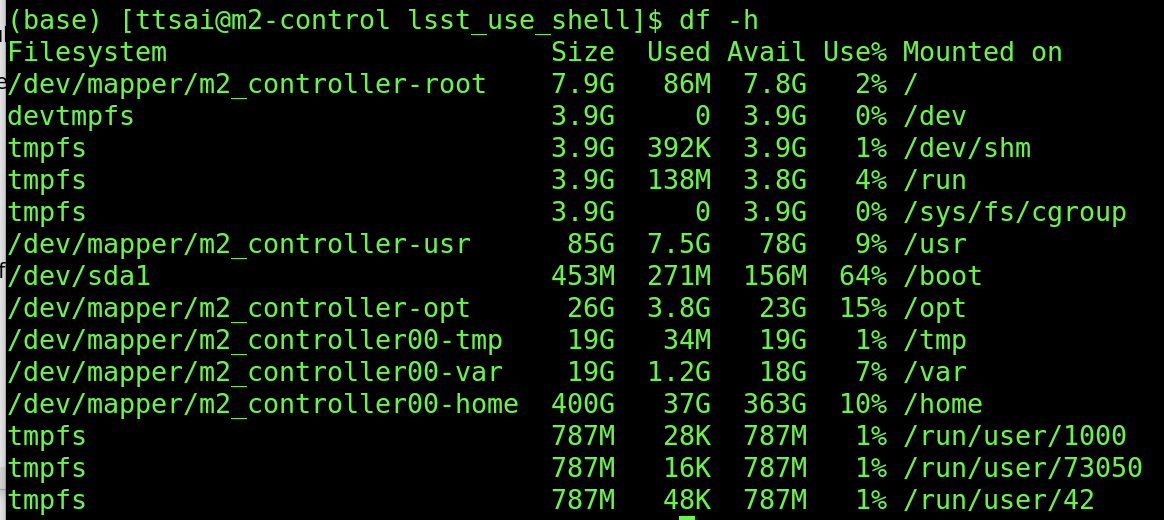
\includegraphics[width=3.54167in]{jira_imgs/1484.png}2. The log and
telemetry files are at ``/home/logs''. They will continue to consume the
disk space when the system runs. To clean the files, you can do ``sh
rmOutOfDateFiles.sh /home/logs'' to remove the files. The shell script
of ``rmOutOfDateFiles.sh'' is under the
``/home/ttsai/Desktop/lsst\_use\_shell'' directory.

}
\hdashrule[0.5ex]{\textwidth}{1pt}{3mm}
  Test Data \\
 {\footnotesize
{Note: This step will be removed in the future as the T\&S team will
provide a script to do the cleaning regularly. In addition, all
telemetry data will be in the summit EFD and the local persistence of
data will be not needed.}

}
\hdashrule[0.5ex]{\textwidth}{1pt}{3mm}
  Expected Result \\
{\footnotesize
The empty space of disk storage is enough to use (\textgreater{} 100
GB).

}
\hdashrule[0.5ex]{\textwidth}{1pt}{3mm}
  Actual Result \\
{\footnotesize

}
\begin{tabular}{p{2cm}p{14cm}}
\toprule
Step 2 & Step Execution Status: \textbf{ Not Executed } \\ \hline
\end{tabular}
 Description \\
{\footnotesize
\textbf{SET UP THE SAL AND \textbf{STARTING THE
EUI}}\\[2\baselineskip]Use the ``ttsai'' account on M2 Dell server at
this moment.\\
1. Use the terminal. Do ``source setM2Sal.sh'' under the
``Desktop/lsst\_use\_shell'' directory. This will set up the SAL 4.x
environment.\\
2. Do ``labview64''. You should see the ``M2Controller.lvproj'' to use.
The repository is at ``/home/ttsai/Documents/github/ts\_mtm2''.\\
3. Click the ``run'' button to execute the M2 control software.\\
4. The system will need some time in initialization. Once it is done,
the user will see the log message of SAL startup. This process could
take 10 - 30 seconds.\\[2\baselineskip]

}
\hdashrule[0.5ex]{\textwidth}{1pt}{3mm}
  Test Data \\
 {\footnotesize
{Note: The T\&S team will provide a formal account (saluser) in a latter
time as discussed in
\href{https://jira.lsstcorp.org/browse/RFC-735}{RFC-735}}

}
\hdashrule[0.5ex]{\textwidth}{1pt}{3mm}
  Expected Result \\
{\footnotesize
The SAL environment is set up and EUI is running.

}
\hdashrule[0.5ex]{\textwidth}{1pt}{3mm}
  Actual Result \\
{\footnotesize

}
\begin{tabular}{p{2cm}p{14cm}}
\toprule
Step 3 & Step Execution Status: \textbf{ Not Executed } \\ \hline
\end{tabular}
 Description \\
{\footnotesize
{Use the chronograf to verify data is being published to the EFD.}

}
\hdashrule[0.5ex]{\textwidth}{1pt}{3mm}
  Test Data \\
 {\footnotesize
Note: If no data is being published to the EFD, contact either Tiago
Ribeiro or Angelo Fausti for help.

}
\hdashrule[0.5ex]{\textwidth}{1pt}{3mm}
  Expected Result \\
{\footnotesize
{Data is being published to the EFD.}

}
\hdashrule[0.5ex]{\textwidth}{1pt}{3mm}
  Actual Result \\
{\footnotesize

}
\begin{tabular}{p{2cm}p{14cm}}
\toprule
Step 4 & Step Execution Status: \textbf{ Not Executed } \\ \hline
\end{tabular}
 Description \\
{\footnotesize
\textbf{SWITCH TO LOCAL CONTROL\\
}\\
Click the ``Local'' button on control panel to switch the system to the
local control. The default local state is the Standby state.\\
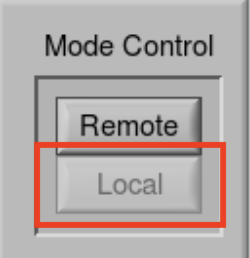
\includegraphics[width=1.07292in]{jira_imgs/1485.png}\\
You can see the state information here:\\
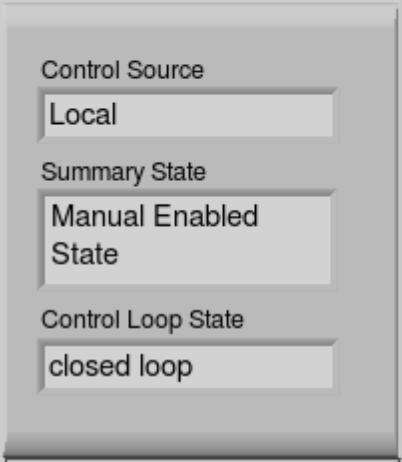
\includegraphics[width=1.09375in]{jira_imgs/1489.png}\\

}
\hdashrule[0.5ex]{\textwidth}{1pt}{3mm}
  Test Data \\
 {\footnotesize
Note: Even though the system is under the local control, it will
continuously publish the telemetry to EFD if the SAL works correctly.

}
\hdashrule[0.5ex]{\textwidth}{1pt}{3mm}
  Expected Result \\
{\footnotesize
The system is under the local control and in Standby state.

}
\hdashrule[0.5ex]{\textwidth}{1pt}{3mm}
  Actual Result \\
{\footnotesize

}
\begin{tabular}{p{2cm}p{14cm}}
\toprule
Step 5 & Step Execution Status: \textbf{ Not Executed } \\ \hline
\end{tabular}
 Description \\
{\footnotesize
\textbf{STANDBY -\textgreater{} DIAGNOSTIC}\\[2\baselineskip]Click the
``Diagnostic'' button on control panel to transition the system to
Diagnostic state.\\
\textbf{\\
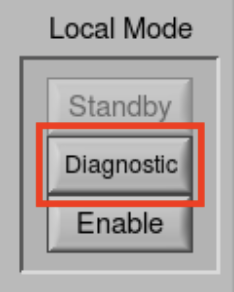
\includegraphics[width=1.07292in]{jira_imgs/1486.png}}

}
\hdashrule[0.5ex]{\textwidth}{1pt}{3mm}
  Expected Result \\
{\footnotesize
The system is in Diagnostic state. The indicator of ``COMM Power'' will
be on as the following:\\
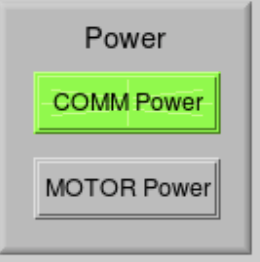
\includegraphics[width=1.20833in]{jira_imgs/1495.png}

}
\hdashrule[0.5ex]{\textwidth}{1pt}{3mm}
  Actual Result \\
{\footnotesize

}
\begin{tabular}{p{2cm}p{14cm}}
\toprule
Step 6 & Step Execution Status: \textbf{ Not Executed } \\ \hline
\end{tabular}
 Description \\
{\footnotesize
\textbf{DIAGNOSTIC \textbf{-\textgreater{}
ENABLE}}\\[2\baselineskip]Click the ``Enable'' button on control panel
to transition the system to Enable state. The system will be under the
open-loop control by default.\\
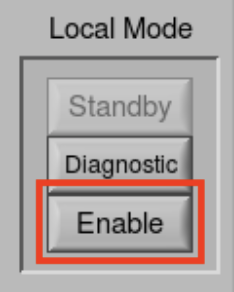
\includegraphics[width=1.02083in]{jira_imgs/1487.png}

}
\hdashrule[0.5ex]{\textwidth}{1pt}{3mm}
  Expected Result \\
{\footnotesize
The system is in Enable state and under the open-loop control. The
indicator of ``MOTOR Power'' will be on as the following:\\
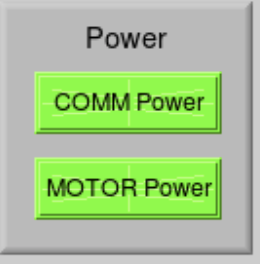
\includegraphics[width=1.23958in]{jira_imgs/1496.png}

}
\hdashrule[0.5ex]{\textwidth}{1pt}{3mm}
  Actual Result \\
{\footnotesize

}
\begin{tabular}{p{2cm}p{14cm}}
\toprule
Step 7 & Step Execution Status: \textbf{ Not Executed } \\ \hline
\end{tabular}
 Description \\
{\footnotesize
\textbf{ENTER THE CLOSED-LOOP CONTROL}\\[2\baselineskip]Click the
``Enter Close-Loop Control'' button to enter the close-loop control
substate.\\
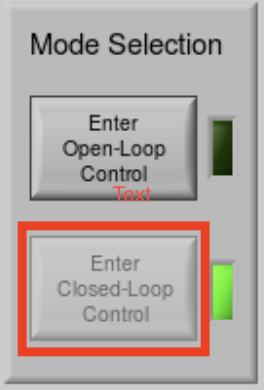
\includegraphics[width=1.10417in]{jira_imgs/1488.png}

}
\hdashrule[0.5ex]{\textwidth}{1pt}{3mm}
  Expected Result \\
{\footnotesize
The system is under the close-loop control.

}
\hdashrule[0.5ex]{\textwidth}{1pt}{3mm}
  Actual Result \\
{\footnotesize

}
\begin{tabular}{p{2cm}p{14cm}}
\toprule
Step 8 & Step Execution Status: \textbf{ Not Executed } \\ \hline
\end{tabular}
 Description \\
{\footnotesize
\textbf{FAULT OCCURRENCE}\\[2\baselineskip]If a fault occurs in any of
the other states, the system will automatically transition to the
Standby state. To clear the error, you need to fix all errors first and
then click the ``Reset All Items'' button. After this, you should be
able to leave the Standby state.

}
\hdashrule[0.5ex]{\textwidth}{1pt}{3mm}
  Expected Result \\
{\footnotesize
The error is cleared and you can do the state transition to Enabled
state.

}
\hdashrule[0.5ex]{\textwidth}{1pt}{3mm}
  Actual Result \\
{\footnotesize

}
\begin{tabular}{p{2cm}p{14cm}}
\toprule
Step 9 & Step Execution Status: \textbf{ Not Executed } \\ \hline
\end{tabular}
 Description \\
{\footnotesize
Verify all mirror sensor signals are displayed on the EUI.

}
\hdashrule[0.5ex]{\textwidth}{1pt}{3mm}
  Expected Result \\
{\footnotesize
The EUI not only displays a summary of the sensor signals but also
provides a summary of the mirror support control system status.

}
\hdashrule[0.5ex]{\textwidth}{1pt}{3mm}
  Actual Result \\
{\footnotesize

}

\paragraph{ LVV-T1613 - M2 Hardware Functional Re-verification }\mbox{}\\

Version \textbf{1}.
Open  \href{https://jira.lsstcorp.org/secure/Tests.jspa#/testCase/LVV-T1613}{\textit{ LVV-T1613 } }
test case in Jira.

The objective of this test case is to re-verify the hardware of the M2.
The M2 hardware was previously checked during some informal, preliminary
testing. This test case will exercise the functionality that was
executed previously and meets the following criteria:~

\begin{itemize}
\tightlist
\item
  Does \textbf{NOT} require the most current version of SAL
\item
  Requires the use of both the EUI and DDS
\item
  Only requires the M2 surrogate to be loaded on the cell
\end{itemize}

\textbf{ Preconditions}:\\


Execution status: {\bf Not Executed }

Final comment:\\


Detailed steps results:

\begin{tabular}{p{2cm}p{14cm}}
\toprule
Step 1 & Step Execution Status: \textbf{ Not Executed } \\ \hline
\end{tabular}
 Description \\
{\footnotesize
\textbf{Inspection}

\begin{itemize}
\tightlist
\item
  Verify the safety stops for the mirror are in place
\item
  Measure the distance between the mirror and the safety stops.
\item
  Measure the distance between the mirror from the aperture ring while
  on the safety stops
\end{itemize}

}
\hdashrule[0.5ex]{\textwidth}{1pt}{3mm}
  Test Data \\
 {\footnotesize
Note: LTS-146 specifies the safety stops should limit the motion of the
mirror to the mirror cell to +/-7.74mm radially and 7.89mm along the
optical axis with a tolerance of 0.5mm.

}
\hdashrule[0.5ex]{\textwidth}{1pt}{3mm}
  Expected Result \\
{\footnotesize
The safety stops are verified to be in place and the distances measured
are within spec.~

}
\hdashrule[0.5ex]{\textwidth}{1pt}{3mm}
  Actual Result \\
{\footnotesize

}
\begin{tabular}{p{2cm}p{14cm}}
\toprule
Step 2 & Step Execution Status: \textbf{ Not Executed } \\ \hline
\end{tabular}
 Description \\
{\footnotesize
Starting from M2 position (0,0,0,0,0,0),\\
move the mirror along x+ direction, with an increment of 0.1mm, and
observe at what point the system goes into fault.

}
\hdashrule[0.5ex]{\textwidth}{1pt}{3mm}
  Expected Result \\
{\footnotesize
The system goes into fault after tripping the positive limit switch.~

}
\hdashrule[0.5ex]{\textwidth}{1pt}{3mm}
  Actual Result \\
{\footnotesize

}
\begin{tabular}{p{2cm}p{14cm}}
\toprule
Step 3 & Step Execution Status: \textbf{ Not Executed } \\ \hline
\end{tabular}
 Description \\
{\footnotesize
Repeat the process for -x direction.

}
\hdashrule[0.5ex]{\textwidth}{1pt}{3mm}
  Expected Result \\
{\footnotesize
The system goes into fault after tripping the negative limit switch.

}
\hdashrule[0.5ex]{\textwidth}{1pt}{3mm}
  Actual Result \\
{\footnotesize

}
\begin{tabular}{p{2cm}p{14cm}}
\toprule
Step 4 & Step Execution Status: \textbf{ Not Executed } \\ \hline
\end{tabular}
 Description \\
{\footnotesize
Repeat the process for +/-y and +/-z directions.

}
\hdashrule[0.5ex]{\textwidth}{1pt}{3mm}
  Expected Result \\
{\footnotesize
There are positive and negative limit switches for the y and z direction
that send the system into fault.~

}
\hdashrule[0.5ex]{\textwidth}{1pt}{3mm}
  Actual Result \\
{\footnotesize

}
\begin{tabular}{p{2cm}p{14cm}}
\toprule
Step 5 & Step Execution Status: \textbf{ Not Executed } \\ \hline
\end{tabular}
 Description \\
{\footnotesize
\textbf{CHECK THE DISK SPACE\\
}\\
Check the disk space in M2 Dell server (public IP:
m2-control.cp.lsst.org).\\
1. Use the terminal. Do ``df -h'' to see the available storage at
``/home'' directory.\\
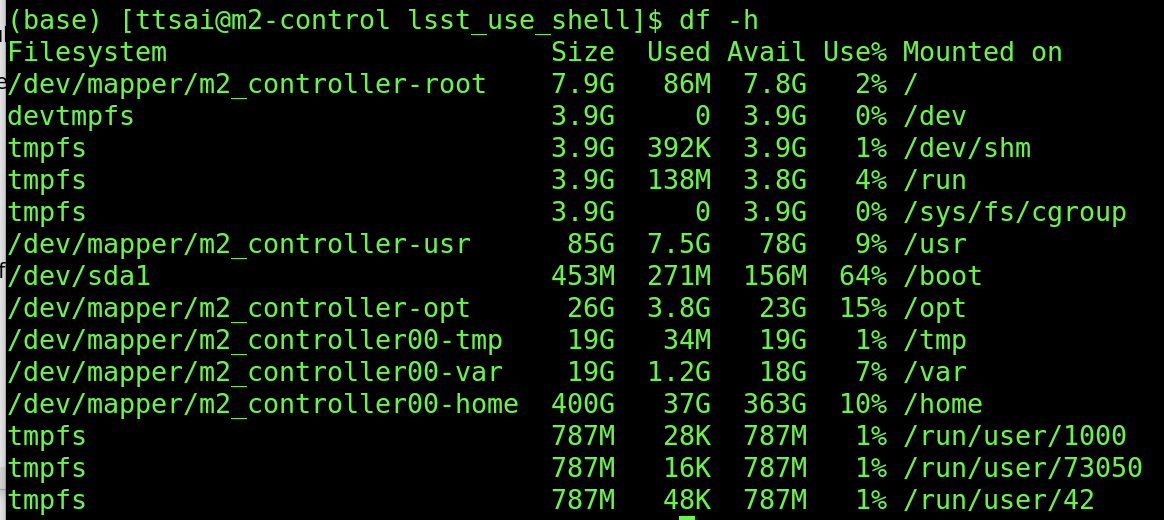
\includegraphics[width=1.56250in]{jira_imgs/1484.png}2. The log and
telemetry files are at ``/home/logs''. They will continue to consume the
disk space when the system runs. To clean the files, you can do ``sh
rmOutOfDateFiles.sh /home/logs'' to remove the files. The shell script
of ``rmOutOfDateFiles.sh'' is under the
``/home/ttsai/Desktop/lsst\_use\_shell'' directory.

}
\hdashrule[0.5ex]{\textwidth}{1pt}{3mm}
  Test Data \\
 {\footnotesize
{Note: This step will be removed in the future as the T\&S team will
provide a script to do the cleaning regularly. In addition, all
telemetry data will be in the summit EFD and the local persistence of
data will be not needed.}

}
\hdashrule[0.5ex]{\textwidth}{1pt}{3mm}
  Expected Result \\
{\footnotesize
The empty space of disk storage is enough to use (\textgreater{} 100
GB).

}
\hdashrule[0.5ex]{\textwidth}{1pt}{3mm}
  Actual Result \\
{\footnotesize

}
\begin{tabular}{p{2cm}p{14cm}}
\toprule
Step 6 & Step Execution Status: \textbf{ Not Executed } \\ \hline
\end{tabular}
 Description \\
{\footnotesize
\textbf{SET UP THE SAL AND \textbf{STARTING THE
EUI}}\\[2\baselineskip]Use the ``ttsai'' account on M2 Dell server at
this moment.\\
1. Use the terminal. Do ``source setM2Sal.sh'' under the
``Desktop/lsst\_use\_shell'' directory. This will set up the SAL 4.x
environment.\\
2. Do ``labview64''. You should see the ``M2Controller.lvproj'' to use.
The repository is at ``/home/ttsai/Documents/github/ts\_mtm2''.\\
3. Click the ``run'' button to execute the M2 control software.\\
4. The system will need some time in initialization. Once it is done,
the user will see the log message of SAL startup. This process could
take 10 - 30 seconds.\\[2\baselineskip]{Note. The T\&S team should
provide a formal account (saluser) in a latter time.}

}
\hdashrule[0.5ex]{\textwidth}{1pt}{3mm}
  Test Data \\
 {\footnotesize
The user will be ``saluser'' as discussed
in~\href{https://jira.lsstcorp.org/browse/RFC-735}{RFC-735}

}
\hdashrule[0.5ex]{\textwidth}{1pt}{3mm}
  Expected Result \\
{\footnotesize
The SAL environment is set up and EUI is running.

}
\hdashrule[0.5ex]{\textwidth}{1pt}{3mm}
  Actual Result \\
{\footnotesize

}
\begin{tabular}{p{2cm}p{14cm}}
\toprule
Step 7 & Step Execution Status: \textbf{ Not Executed } \\ \hline
\end{tabular}
 Description \\
{\footnotesize
Use the chronograf to verify data is being published to the EFD.

}
\hdashrule[0.5ex]{\textwidth}{1pt}{3mm}
  Test Data \\
 {\footnotesize
Note: If no data is being published to the EFD, contact either Tiago
Ribeiro or Angelo Fausti for help.

}
\hdashrule[0.5ex]{\textwidth}{1pt}{3mm}
  Expected Result \\
{\footnotesize
{Data is being published to the EFD}

}
\hdashrule[0.5ex]{\textwidth}{1pt}{3mm}
  Actual Result \\
{\footnotesize

}
\begin{tabular}{p{2cm}p{14cm}}
\toprule
Step 8 & Step Execution Status: \textbf{ Not Executed } \\ \hline
\end{tabular}
 Description \\
{\footnotesize
\textbf{REMOTE CONTROL}\\[2\baselineskip]The system should be in the
remote control by default. The initial substate is Offline/PublishOnly.
If the system passes all the checking, it will transition to
Offline/AvailableState substate. You can see the state information
here:\\
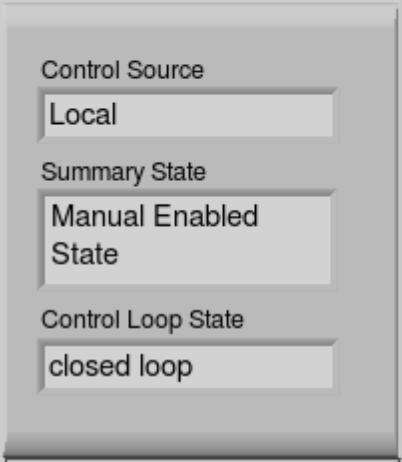
\includegraphics[width=1.30208in]{jira_imgs/1490.png}\textbf{\\
}

}
\hdashrule[0.5ex]{\textwidth}{1pt}{3mm}
  Test Data \\
 {\footnotesize
Note: The M2 control system was updated so that it could be transitioned
from Offline/PublishOnly to Offline/AvailableState as discussed
in~\href{https://jira.lsstcorp.org/browse/DM-2729}{DM-27291}

}
\hdashrule[0.5ex]{\textwidth}{1pt}{3mm}
  Expected Result \\
{\footnotesize
The system is under the remote control and in Offline/AvailableState
substate.

}
\hdashrule[0.5ex]{\textwidth}{1pt}{3mm}
  Actual Result \\
{\footnotesize

}
\begin{tabular}{p{2cm}p{14cm}}
\toprule
Step 9 & Step Execution Status: \textbf{ Not Executed } \\ \hline
\end{tabular}
 Description \\
{\footnotesize
\textbf{OFFLINE -\textgreater{} STANDBY}\\[2\baselineskip]The system
receives an\emph{~enterControl~}command through SAL.

}
\hdashrule[0.5ex]{\textwidth}{1pt}{3mm}
  Expected Result \\
{\footnotesize
The system transitions into the Standby state and is capable of
receiving/responding to DDS commands.

}
\hdashrule[0.5ex]{\textwidth}{1pt}{3mm}
  Actual Result \\
{\footnotesize

}
\begin{tabular}{p{2cm}p{14cm}}
\toprule
Step 10 & Step Execution Status: \textbf{ Not Executed } \\ \hline
\end{tabular}
 Description \\
{\footnotesize
\textbf{STANDBY -\textgreater{} DISABLED}\\[2\baselineskip]From the
Standby state, send a \emph{start~}command through the DDS.

}
\hdashrule[0.5ex]{\textwidth}{1pt}{3mm}
  Expected Result \\
{\footnotesize
The system transitions into the Disabled state and is capable of
receiving/responding to DDS commands. The indicator of ``COMM Power''
will be on as the following:\\
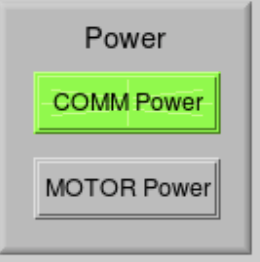
\includegraphics[width=1.21875in]{jira_imgs/1494.png}

}
\hdashrule[0.5ex]{\textwidth}{1pt}{3mm}
  Actual Result \\
{\footnotesize

}
\begin{tabular}{p{2cm}p{14cm}}
\toprule
Step 11 & Step Execution Status: \textbf{ Not Executed } \\ \hline
\end{tabular}
 Description \\
{\footnotesize
\textbf{DISABLED -\textgreater{} ENABLED}\\[2\baselineskip]From the
Disabled state, send an \emph{enable state~}command through the DDS.

}
\hdashrule[0.5ex]{\textwidth}{1pt}{3mm}
  Expected Result \\
{\footnotesize
The system transitions into the Enabled state and is capable of
receiving/responding to DDS commands. The indicator of ``MOTOR Power''
will be on as the following:\\
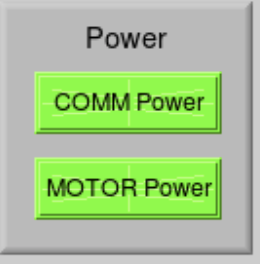
\includegraphics[width=1.16667in]{jira_imgs/1496.png}\\[2\baselineskip]The
system will be in the close-loop control mode. This is different from
the local mode. In the remote control, only the close-loop control is
allowed.

}
\hdashrule[0.5ex]{\textwidth}{1pt}{3mm}
  Actual Result \\
{\footnotesize

}
\begin{tabular}{p{2cm}p{14cm}}
\toprule
Step 12 & Step Execution Status: \textbf{ Not Executed } \\ \hline
\end{tabular}
 Description \\
{\footnotesize
\textbf{FAULT STATE}\\[2\baselineskip]If a fault occurs in any of the
other states, the system will automatically transition to the Fault
state. While in the Fault state, send a \emph{clearErrors~}command
through the DDS.

}
\hdashrule[0.5ex]{\textwidth}{1pt}{3mm}
  Expected Result \\
{\footnotesize
The system transitions to the Standby state.

}
\hdashrule[0.5ex]{\textwidth}{1pt}{3mm}
  Actual Result \\
{\footnotesize

}
\begin{tabular}{p{2cm}p{14cm}}
\toprule
Step 13 & Step Execution Status: \textbf{ Not Executed } \\ \hline
\end{tabular}
 Description \\
{\footnotesize
\textbf{CHECK THE DISK SPACE\\
}\\
Check the disk space in M2 Dell server (public IP:
m2-control.cp.lsst.org).\\
1. Use the terminal. Do ``df -h'' to see the available storage at
``/home'' directory.\\
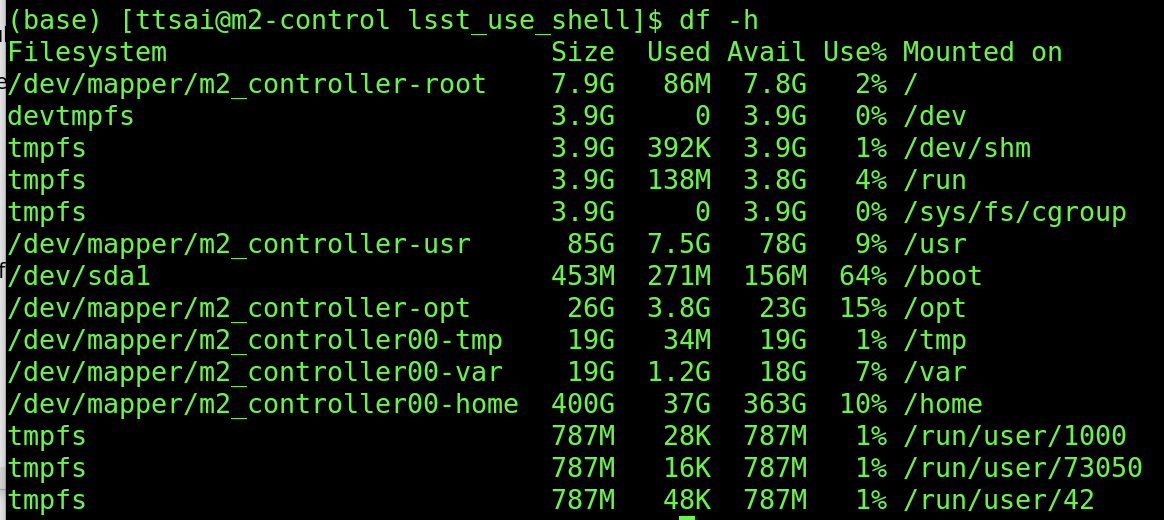
\includegraphics[width=3.54167in]{jira_imgs/1484.png}2. The log and
telemetry files are at ``/home/logs''. They will continue to consume the
disk space when the system runs. To clean the files, you can do ``sh
rmOutOfDateFiles.sh /home/logs'' to remove the files. The shell script
of ``rmOutOfDateFiles.sh'' is under the
``/home/ttsai/Desktop/lsst\_use\_shell'' directory.

}
\hdashrule[0.5ex]{\textwidth}{1pt}{3mm}
  Test Data \\
 {\footnotesize
{Note: This step will be removed in the future as the T\&S team will
provide a script to do the cleaning regularly. In addition, all
telemetry data will be in the summit EFD and the local persistence of
data will be not needed.}

}
\hdashrule[0.5ex]{\textwidth}{1pt}{3mm}
  Expected Result \\
{\footnotesize
The empty space of disk storage is enough to use (\textgreater{} 100
GB).

}
\hdashrule[0.5ex]{\textwidth}{1pt}{3mm}
  Actual Result \\
{\footnotesize

}
\begin{tabular}{p{2cm}p{14cm}}
\toprule
Step 14 & Step Execution Status: \textbf{ Not Executed } \\ \hline
\end{tabular}
 Description \\
{\footnotesize
\textbf{SET UP THE SAL AND \textbf{STARTING THE
EUI}}\\[2\baselineskip]Use the ``ttsai'' account on M2 Dell server at
this moment.\\
1. Use the terminal. Do ``source setM2Sal.sh'' under the
``Desktop/lsst\_use\_shell'' directory. This will set up the SAL 4.x
environment.\\
2. Do ``labview64''. You should see the ``M2Controller.lvproj'' to use.
The repository is at ``/home/ttsai/Documents/github/ts\_mtm2''.\\
3. Click the ``run'' button to execute the M2 control software.\\
4. The system will need some time in initialization. Once it is done,
the user will see the log message of SAL startup. This process could
take 10 - 30 seconds.\\[2\baselineskip]

}
\hdashrule[0.5ex]{\textwidth}{1pt}{3mm}
  Test Data \\
 {\footnotesize
{Note: The T\&S team will provide a formal account (saluser) in a latter
time as discussed in
\href{https://jira.lsstcorp.org/browse/RFC-735}{RFC-735}}

}
\hdashrule[0.5ex]{\textwidth}{1pt}{3mm}
  Expected Result \\
{\footnotesize
The SAL environment is set up and EUI is running.

}
\hdashrule[0.5ex]{\textwidth}{1pt}{3mm}
  Actual Result \\
{\footnotesize

}
\begin{tabular}{p{2cm}p{14cm}}
\toprule
Step 15 & Step Execution Status: \textbf{ Not Executed } \\ \hline
\end{tabular}
 Description \\
{\footnotesize
{Use the chronograf to verify data is being published to the EFD.}

}
\hdashrule[0.5ex]{\textwidth}{1pt}{3mm}
  Test Data \\
 {\footnotesize
Note: If no data is being published to the EFD, contact either Tiago
Ribeiro or Angelo Fausti for help.

}
\hdashrule[0.5ex]{\textwidth}{1pt}{3mm}
  Expected Result \\
{\footnotesize
{Data is being published to the EFD.}

}
\hdashrule[0.5ex]{\textwidth}{1pt}{3mm}
  Actual Result \\
{\footnotesize

}
\begin{tabular}{p{2cm}p{14cm}}
\toprule
Step 16 & Step Execution Status: \textbf{ Not Executed } \\ \hline
\end{tabular}
 Description \\
{\footnotesize
\textbf{SWITCH TO LOCAL CONTROL\\
}\\
Click the ``Local'' button on control panel to switch the system to the
local control. The default local state is the Standby state.\\
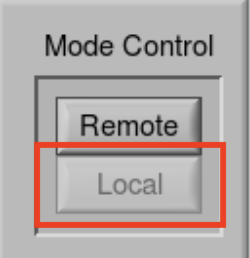
\includegraphics[width=1.07292in]{jira_imgs/1485.png}\\
You can see the state information here:\\
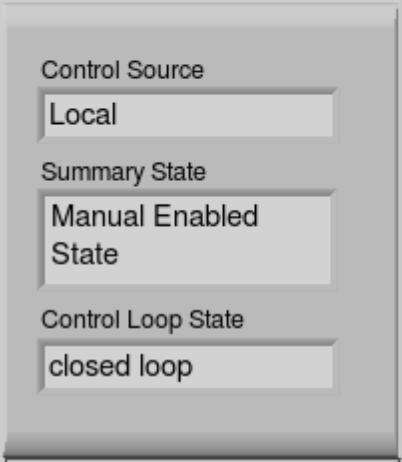
\includegraphics[width=1.09375in]{jira_imgs/1489.png}\\

}
\hdashrule[0.5ex]{\textwidth}{1pt}{3mm}
  Test Data \\
 {\footnotesize
Note: Even though the system is under the local control, it will
continuously publish the telemetry to EFD if the SAL works correctly.

}
\hdashrule[0.5ex]{\textwidth}{1pt}{3mm}
  Expected Result \\
{\footnotesize
The system is under the local control and in Standby state.

}
\hdashrule[0.5ex]{\textwidth}{1pt}{3mm}
  Actual Result \\
{\footnotesize

}
\begin{tabular}{p{2cm}p{14cm}}
\toprule
Step 17 & Step Execution Status: \textbf{ Not Executed } \\ \hline
\end{tabular}
 Description \\
{\footnotesize
\textbf{STANDBY -\textgreater{} DIAGNOSTIC}\\[2\baselineskip]Click the
``Diagnostic'' button on control panel to transition the system to
Diagnostic state.\\
\textbf{\\
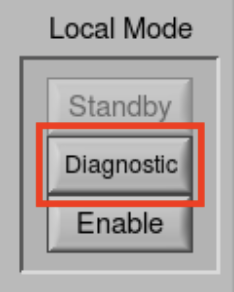
\includegraphics[width=1.07292in]{jira_imgs/1486.png}}

}
\hdashrule[0.5ex]{\textwidth}{1pt}{3mm}
  Expected Result \\
{\footnotesize
The system is in Diagnostic state. The indicator of ``COMM Power'' will
be on as the following:\\
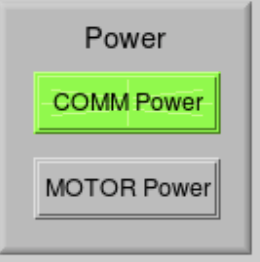
\includegraphics[width=1.20833in]{jira_imgs/1495.png}

}
\hdashrule[0.5ex]{\textwidth}{1pt}{3mm}
  Actual Result \\
{\footnotesize

}
\begin{tabular}{p{2cm}p{14cm}}
\toprule
Step 18 & Step Execution Status: \textbf{ Not Executed } \\ \hline
\end{tabular}
 Description \\
{\footnotesize
\textbf{DIAGNOSTIC \textbf{-\textgreater{}
ENABLE}}\\[2\baselineskip]Click the ``Enable'' button on control panel
to transition the system to Enable state. The system will be under the
open-loop control by default.\\
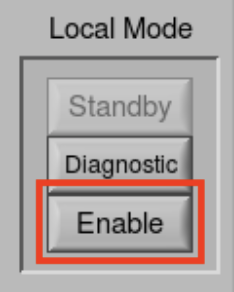
\includegraphics[width=1.02083in]{jira_imgs/1487.png}

}
\hdashrule[0.5ex]{\textwidth}{1pt}{3mm}
  Expected Result \\
{\footnotesize
The system is in Enable state and under the open-loop control. The
indicator of ``MOTOR Power'' will be on as the following:\\
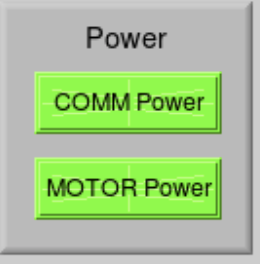
\includegraphics[width=1.23958in]{jira_imgs/1496.png}

}
\hdashrule[0.5ex]{\textwidth}{1pt}{3mm}
  Actual Result \\
{\footnotesize

}
\begin{tabular}{p{2cm}p{14cm}}
\toprule
Step 19 & Step Execution Status: \textbf{ Not Executed } \\ \hline
\end{tabular}
 Description \\
{\footnotesize
\textbf{ENTER THE CLOSED-LOOP CONTROL}\\[2\baselineskip]Click the
``Enter Close-Loop Control'' button to enter the close-loop control
substate.\\
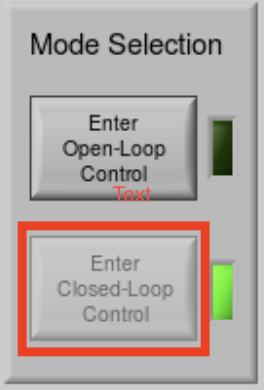
\includegraphics[width=1.10417in]{jira_imgs/1488.png}

}
\hdashrule[0.5ex]{\textwidth}{1pt}{3mm}
  Expected Result \\
{\footnotesize
The system is under the close-loop control.

}
\hdashrule[0.5ex]{\textwidth}{1pt}{3mm}
  Actual Result \\
{\footnotesize

}
\begin{tabular}{p{2cm}p{14cm}}
\toprule
Step 20 & Step Execution Status: \textbf{ Not Executed } \\ \hline
\end{tabular}
 Description \\
{\footnotesize
\textbf{FAULT OCCURRENCE}\\[2\baselineskip]If a fault occurs in any of
the other states, the system will automatically transition to the
Standby state. To clear the error, you need to fix all errors first and
then click the ``Reset All Items'' button. After this, you should be
able to leave the Standby state.

}
\hdashrule[0.5ex]{\textwidth}{1pt}{3mm}
  Expected Result \\
{\footnotesize
The error is cleared and you can do the state transition to Enabled
state.

}
\hdashrule[0.5ex]{\textwidth}{1pt}{3mm}
  Actual Result \\
{\footnotesize

}

\paragraph{ LVV-T1615 - Integration of M2 with SAL }\mbox{}\\

Version \textbf{1}.
Open  \href{https://jira.lsstcorp.org/secure/Tests.jspa#/testCase/LVV-T1615}{\textit{ LVV-T1615 } }
test case in Jira.

The objective of this test case is to verify the software requirements
of the M2 cell, as defined in \citeds{LTS-146} and \citeds{LTS-162}, utilizing the updated
M2 CSC (SAL). The software requirements were previously verified during
the test campaign by the vendor, but have since been updated per
CR-0202. This test case will exercise the functionality of the M2 CSC
and meets the following criteria:

\begin{itemize}
\tightlist
\item
  Only requires the most current version of SAL
\item
  Only requires the M2 surrogate to be loaded on the cell
\item
  Requires the use of both the EUI and DDS
\item
  Does \textbf{NOT~}require the M2 to be integrated with the Interlock
  system
\end{itemize}

\textbf{ Preconditions}:\\


Execution status: {\bf Not Executed }

Final comment:\\


Detailed steps results:

\begin{tabular}{p{2cm}p{14cm}}
\toprule
Step 1 & Step Execution Status: \textbf{ Not Executed } \\ \hline
\end{tabular}
 Description \\
{\footnotesize
\textbf{CHECK THE DISK SPACE\\
}\\
Check the disk space in M2 Dell server (public IP:
m2-control.cp.lsst.org).\\
1. Use the terminal. Do ``df -h'' to see the available storage at
``/home'' directory.\\
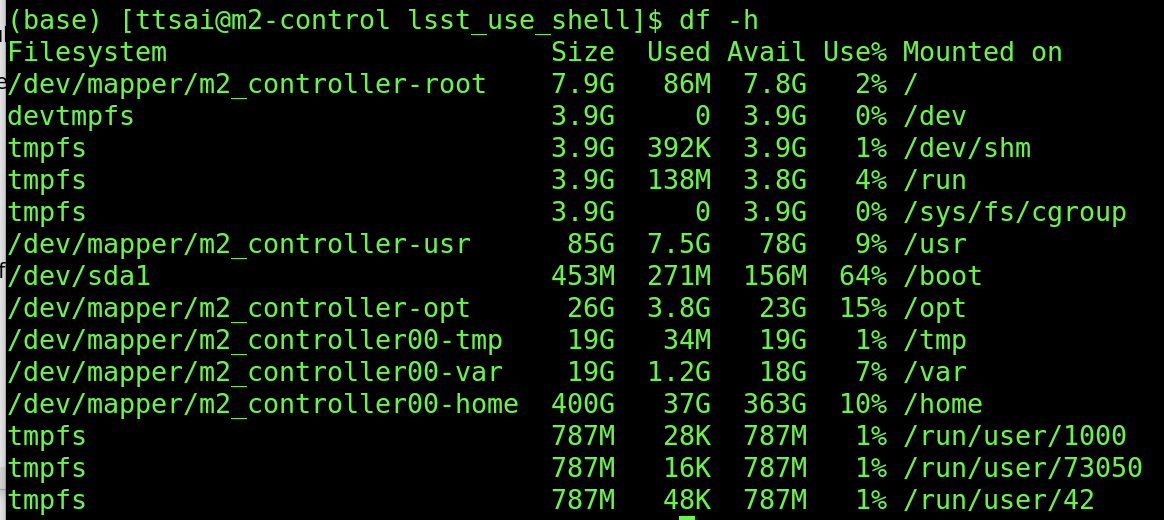
\includegraphics[width=1.56250in]{jira_imgs/1484.png}2. The log and
telemetry files are at ``/home/logs''. They will continue to consume the
disk space when the system runs. To clean the files, you can do ``sh
rmOutOfDateFiles.sh /home/logs'' to remove the files. The shell script
of ``rmOutOfDateFiles.sh'' is under the
``/home/ttsai/Desktop/lsst\_use\_shell'' directory.

}
\hdashrule[0.5ex]{\textwidth}{1pt}{3mm}
  Test Data \\
 {\footnotesize
{Note: This step will be removed in the future as the T\&S team will
provide a script to do the cleaning regularly. In addition, all
telemetry data will be in the summit EFD and the local persistence of
data will be not needed.}

}
\hdashrule[0.5ex]{\textwidth}{1pt}{3mm}
  Expected Result \\
{\footnotesize
The empty space of disk storage is enough to use (\textgreater{} 100
GB).

}
\hdashrule[0.5ex]{\textwidth}{1pt}{3mm}
  Actual Result \\
{\footnotesize

}
\begin{tabular}{p{2cm}p{14cm}}
\toprule
Step 2 & Step Execution Status: \textbf{ Not Executed } \\ \hline
\end{tabular}
 Description \\
{\footnotesize
\textbf{SET UP THE SAL AND \textbf{STARTING THE
EUI}}\\[2\baselineskip]Use the ``ttsai'' account on M2 Dell server at
this moment.\\
1. Use the terminal. Do ``source setM2Sal.sh'' under the
``Desktop/lsst\_use\_shell'' directory. This will set up the SAL 4.x
environment.\\
2. Do ``labview64''. You should see the ``M2Controller.lvproj'' to use.
The repository is at ``/home/ttsai/Documents/github/ts\_mtm2''.\\
3. Click the ``run'' button to execute the M2 control software.\\
4. The system will need some time in initialization. Once it is done,
the user will see the log message of SAL startup. This process could
take 10 - 30 seconds.\\[2\baselineskip]{Note. The T\&S team should
provide a formal account (saluser) in a latter time.}

}
\hdashrule[0.5ex]{\textwidth}{1pt}{3mm}
  Test Data \\
 {\footnotesize
The user will be ``saluser'' as discussed
in~\href{https://jira.lsstcorp.org/browse/RFC-735}{RFC-735}

}
\hdashrule[0.5ex]{\textwidth}{1pt}{3mm}
  Expected Result \\
{\footnotesize
The SAL environment is set up and EUI is running.

}
\hdashrule[0.5ex]{\textwidth}{1pt}{3mm}
  Actual Result \\
{\footnotesize

}
\begin{tabular}{p{2cm}p{14cm}}
\toprule
Step 3 & Step Execution Status: \textbf{ Not Executed } \\ \hline
\end{tabular}
 Description \\
{\footnotesize
Use the chronograf to verify data is being published to the EFD.

}
\hdashrule[0.5ex]{\textwidth}{1pt}{3mm}
  Test Data \\
 {\footnotesize
Note: If no data is being published to the EFD, contact either Tiago
Ribeiro or Angelo Fausti for help.

}
\hdashrule[0.5ex]{\textwidth}{1pt}{3mm}
  Expected Result \\
{\footnotesize
{Data is being published to the EFD}

}
\hdashrule[0.5ex]{\textwidth}{1pt}{3mm}
  Actual Result \\
{\footnotesize

}
\begin{tabular}{p{2cm}p{14cm}}
\toprule
Step 4 & Step Execution Status: \textbf{ Not Executed } \\ \hline
\end{tabular}
 Description \\
{\footnotesize
\textbf{REMOTE CONTROL}\\[2\baselineskip]The system should be in the
remote control by default. The initial substate is Offline/PublishOnly.
If the system passes all the checking, it will transition to
Offline/AvailableState substate. You can see the state information
here:\\
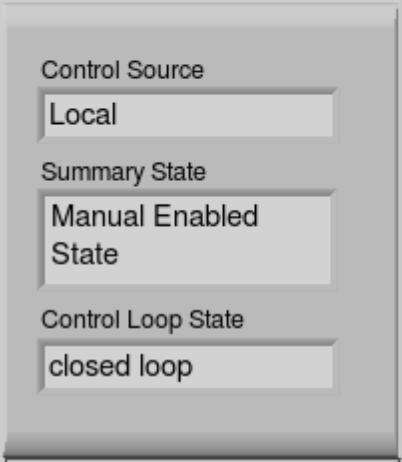
\includegraphics[width=1.30208in]{jira_imgs/1490.png}\textbf{\\
}

}
\hdashrule[0.5ex]{\textwidth}{1pt}{3mm}
  Test Data \\
 {\footnotesize
Note: The M2 control system was updated so that it could be transitioned
from Offline/PublishOnly to Offline/AvailableState as discussed
in~\href{https://jira.lsstcorp.org/browse/DM-2729}{DM-27291}

}
\hdashrule[0.5ex]{\textwidth}{1pt}{3mm}
  Expected Result \\
{\footnotesize
The system is under the remote control and in Offline/AvailableState
substate.

}
\hdashrule[0.5ex]{\textwidth}{1pt}{3mm}
  Actual Result \\
{\footnotesize

}
\begin{tabular}{p{2cm}p{14cm}}
\toprule
Step 5 & Step Execution Status: \textbf{ Not Executed } \\ \hline
\end{tabular}
 Description \\
{\footnotesize
\textbf{OFFLINE -\textgreater{} STANDBY}\\[2\baselineskip]The system
receives an\emph{~enterControl~}command through SAL.

}
\hdashrule[0.5ex]{\textwidth}{1pt}{3mm}
  Expected Result \\
{\footnotesize
The system transitions into the Standby state and is capable of
receiving/responding to DDS commands.

}
\hdashrule[0.5ex]{\textwidth}{1pt}{3mm}
  Actual Result \\
{\footnotesize

}
\begin{tabular}{p{2cm}p{14cm}}
\toprule
Step 6 & Step Execution Status: \textbf{ Not Executed } \\ \hline
\end{tabular}
 Description \\
{\footnotesize
\textbf{STANDBY -\textgreater{} DISABLED}\\[2\baselineskip]From the
Standby state, send a \emph{start~}command through the DDS.

}
\hdashrule[0.5ex]{\textwidth}{1pt}{3mm}
  Expected Result \\
{\footnotesize
The system transitions into the Disabled state and is capable of
receiving/responding to DDS commands. The indicator of ``COMM Power''
will be on as the following:\\
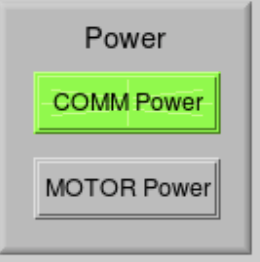
\includegraphics[width=1.21875in]{jira_imgs/1494.png}

}
\hdashrule[0.5ex]{\textwidth}{1pt}{3mm}
  Actual Result \\
{\footnotesize

}
\begin{tabular}{p{2cm}p{14cm}}
\toprule
Step 7 & Step Execution Status: \textbf{ Not Executed } \\ \hline
\end{tabular}
 Description \\
{\footnotesize
\textbf{DISABLED -\textgreater{} ENABLED}\\[2\baselineskip]From the
Disabled state, send an \emph{enable state~}command through the DDS.

}
\hdashrule[0.5ex]{\textwidth}{1pt}{3mm}
  Expected Result \\
{\footnotesize
The system transitions into the Enabled state and is capable of
receiving/responding to DDS commands. The indicator of ``MOTOR Power''
will be on as the following:\\
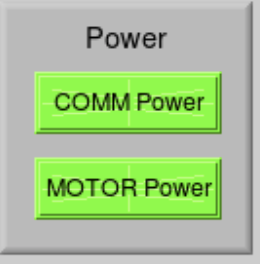
\includegraphics[width=1.16667in]{jira_imgs/1496.png}\\[2\baselineskip]The
system will be in the close-loop control mode. This is different from
the local mode. In the remote control, only the close-loop control is
allowed.

}
\hdashrule[0.5ex]{\textwidth}{1pt}{3mm}
  Actual Result \\
{\footnotesize

}
\begin{tabular}{p{2cm}p{14cm}}
\toprule
Step 8 & Step Execution Status: \textbf{ Not Executed } \\ \hline
\end{tabular}
 Description \\
{\footnotesize
\textbf{FAULT STATE}\\[2\baselineskip]If a fault occurs in any of the
other states, the system will automatically transition to the Fault
state. While in the Fault state, send a \emph{clearErrors~}command
through the DDS.

}
\hdashrule[0.5ex]{\textwidth}{1pt}{3mm}
  Expected Result \\
{\footnotesize
The system transitions to the Standby state.

}
\hdashrule[0.5ex]{\textwidth}{1pt}{3mm}
  Actual Result \\
{\footnotesize

}
\begin{tabular}{p{2cm}p{14cm}}
\toprule
Step 9 & Step Execution Status: \textbf{ Not Executed } \\ \hline
\end{tabular}
 Description \\
{\footnotesize
\textbf{ApplyForces command}\\[2\baselineskip]Before sending the
ApplyForces command, take note of the force telemetry output by the EFD.

}
\hdashrule[0.5ex]{\textwidth}{1pt}{3mm}
  Expected Result \\
{\footnotesize
The force telemetry should reflect the forces applied by the LUT. This
will be seen as the initial condition.

}
\hdashrule[0.5ex]{\textwidth}{1pt}{3mm}
  Actual Result \\
{\footnotesize

}
\begin{tabular}{p{2cm}p{14cm}}
\toprule
Step 10 & Step Execution Status: \textbf{ Not Executed } \\ \hline
\end{tabular}
 Description \\
{\footnotesize
In the Enabled State and closed-loop mode, send the ApplyForces command
over SAL.

}
\hdashrule[0.5ex]{\textwidth}{1pt}{3mm}
  Test Data \\
 {\footnotesize
Force should not be applied to the axial actuators at the same time as
the tangential actuators. Make sure the summation of forces in the
Z-direction is zero. The forces applied should not be random values. As
an example, apply bending modes 1-20.

}
\hdashrule[0.5ex]{\textwidth}{1pt}{3mm}
  Expected Result \\
{\footnotesize
The force telemetry should show the combined value of forces from the
initial condition and the forces commanded through SAL. The difference
between the force telemetry between now and the initial condition should
equal the forces sent through the ApplyForces command.~

}
\hdashrule[0.5ex]{\textwidth}{1pt}{3mm}
  Actual Result \\
{\footnotesize

}
\begin{tabular}{p{2cm}p{14cm}}
\toprule
Step 11 & Step Execution Status: \textbf{ Not Executed } \\ \hline
\end{tabular}
 Description \\
{\footnotesize
\textbf{ResetForceOffsets}\\[2\baselineskip]Send the ResetForceOffsets
command through SAL.

}
\hdashrule[0.5ex]{\textwidth}{1pt}{3mm}
  Test Data \\
 {\footnotesize
This should be done after a successful ApplyForces command.~

}
\hdashrule[0.5ex]{\textwidth}{1pt}{3mm}
  Expected Result \\
{\footnotesize
Force telemetry should show a difference from when the ApplyForces
command was issued to after the resetforceoffsets command is issued. The
78 nonzero force values are now zero.~

}
\hdashrule[0.5ex]{\textwidth}{1pt}{3mm}
  Actual Result \\
{\footnotesize

}
\begin{tabular}{p{2cm}p{14cm}}
\toprule
Step 12 & Step Execution Status: \textbf{ Not Executed } \\ \hline
\end{tabular}
 Description \\
{\footnotesize
\textbf{PositionMirror command}\\[2\baselineskip]In the enabled state
and closed loop mode, send a position command of 100um, 100um, 100um,
100urad, 100urad, 100urad

}
\hdashrule[0.5ex]{\textwidth}{1pt}{3mm}
  Test Data \\
 {\footnotesize
Note: There will be two types of telemetry - one measured by the
hardpoints and one measured by the IMS\\
This specific position was selected because it should be within the
limits so the positionMirror command can be verified without running
into an error.

}
\hdashrule[0.5ex]{\textwidth}{1pt}{3mm}
  Expected Result \\
{\footnotesize
\begin{itemize}
\tightlist
\item
  The telemetry data reported by the hardpoints and by the IMS is
  consistent to the position command given.~
\item
  The inPosition event is published as true.
\end{itemize}

}
\hdashrule[0.5ex]{\textwidth}{1pt}{3mm}
  Actual Result \\
{\footnotesize

}
\begin{tabular}{p{2cm}p{14cm}}
\toprule
Step 13 & Step Execution Status: \textbf{ Not Executed } \\ \hline
\end{tabular}
 Description \\
{\footnotesize
\textbf{ClearError command}\\
Unplug the cable to actuator A1.

}
\hdashrule[0.5ex]{\textwidth}{1pt}{3mm}
  Test Data \\
 {\footnotesize
A Mechanical Engineer must be present in order to unplug the actuator.

}
\hdashrule[0.5ex]{\textwidth}{1pt}{3mm}
  Expected Result \\
{\footnotesize
System goes into a ``FAULT'' state and is indicated by a red light on
the EUI.~

}
\hdashrule[0.5ex]{\textwidth}{1pt}{3mm}
  Actual Result \\
{\footnotesize

}
\begin{tabular}{p{2cm}p{14cm}}
\toprule
Step 14 & Step Execution Status: \textbf{ Not Executed } \\ \hline
\end{tabular}
 Description \\
{\footnotesize
send ClearErrors command~

}
\hdashrule[0.5ex]{\textwidth}{1pt}{3mm}
  Expected Result \\
{\footnotesize
the ClearErrors command allows the system to transition out of FAULT
state and is able to re-enter Enabled/closed loop mode~

}
\hdashrule[0.5ex]{\textwidth}{1pt}{3mm}
  Actual Result \\
{\footnotesize

}
\begin{tabular}{p{2cm}p{14cm}}
\toprule
Step 15 & Step Execution Status: \textbf{ Not Executed } \\ \hline
\end{tabular}
 Description \\
{\footnotesize
\textbf{M2 Assembly detailed state}\\[2\baselineskip]Verify the detailed
state event is published after each state transition.

}
\hdashrule[0.5ex]{\textwidth}{1pt}{3mm}
  Expected Result \\
{\footnotesize
The M2 Assembly publishes the values of the new detailed state on each
detailed state transition

}
\hdashrule[0.5ex]{\textwidth}{1pt}{3mm}
  Actual Result \\
{\footnotesize

}
\begin{tabular}{p{2cm}p{14cm}}
\toprule
Step 16 & Step Execution Status: \textbf{ Not Executed } \\ \hline
\end{tabular}
 Description \\
{\footnotesize
\textbf{M2 Assembly inPosition}\\[2\baselineskip]Verify that inPosition
event is published as a result of the positionMirror Command

}
\hdashrule[0.5ex]{\textwidth}{1pt}{3mm}
  Test Data \\
 {\footnotesize
Mark this step as pass if the positionMirror command step is passed

}
\hdashrule[0.5ex]{\textwidth}{1pt}{3mm}
  Expected Result \\
{\footnotesize
The inPosition event is published as true when the mirror has reached
the~

}
\hdashrule[0.5ex]{\textwidth}{1pt}{3mm}
  Actual Result \\
{\footnotesize

}
\begin{tabular}{p{2cm}p{14cm}}
\toprule
Step 17 & Step Execution Status: \textbf{ Not Executed } \\ \hline
\end{tabular}
 Description \\
{\footnotesize
\textbf{CellTemperatureHiWarning}\\[2\baselineskip]Take note of the
CellTemperatureHiWarning event.

}
\hdashrule[0.5ex]{\textwidth}{1pt}{3mm}
  Expected Result \\
{\footnotesize
The CellTemperatureHiWarning event is published and reads false.

}
\hdashrule[0.5ex]{\textwidth}{1pt}{3mm}
  Actual Result \\
{\footnotesize

}
\begin{tabular}{p{2cm}p{14cm}}
\toprule
Step 18 & Step Execution Status: \textbf{ Not Executed } \\ \hline
\end{tabular}
 Description \\
{\footnotesize
First verify which value corresponds to which sensor.

}
\hdashrule[0.5ex]{\textwidth}{1pt}{3mm}
  Expected Result \\
{\footnotesize
The values corresponding to each sensor are known

}
\hdashrule[0.5ex]{\textwidth}{1pt}{3mm}
  Actual Result \\
{\footnotesize

}
\begin{tabular}{p{2cm}p{14cm}}
\toprule
Step 19 & Step Execution Status: \textbf{ Not Executed } \\ \hline
\end{tabular}
 Description \\
{\footnotesize
Use hot plate/heat gun/hair dryer (\textbf{TBD}) to heat the sensor
measuring the exhaust air temperature.~

}
\hdashrule[0.5ex]{\textwidth}{1pt}{3mm}
  Test Data \\
 {\footnotesize
The default delta is changed from the required 2.0deg to 0.5deg for
safety reasons.

}
\hdashrule[0.5ex]{\textwidth}{1pt}{3mm}
  Expected Result \\
{\footnotesize
The CellTemperatureHiWarning event is published and reads true.~

}
\hdashrule[0.5ex]{\textwidth}{1pt}{3mm}
  Actual Result \\
{\footnotesize

}
\begin{tabular}{p{2cm}p{14cm}}
\toprule
Step 20 & Step Execution Status: \textbf{ Not Executed } \\ \hline
\end{tabular}
 Description \\
{\footnotesize
Use ice cube (\textbf{not really;~TBD}) to cool the sensor measuring the
exhaust air temperature

}
\hdashrule[0.5ex]{\textwidth}{1pt}{3mm}
  Expected Result \\
{\footnotesize
The CellTemperatureHiWarning event is published and reads false.~

}
\hdashrule[0.5ex]{\textwidth}{1pt}{3mm}
  Actual Result \\
{\footnotesize

}
\begin{tabular}{p{2cm}p{14cm}}
\toprule
Step 21 & Step Execution Status: \textbf{ Not Executed } \\ \hline
\end{tabular}
 Description \\
{\footnotesize
\textbf{Commandable by DDS}\\[2\baselineskip]{Take note that of the EFD
while M2 is controlled by EUI.}

}
\hdashrule[0.5ex]{\textwidth}{1pt}{3mm}
  Test Data \\
 {\footnotesize
Confirm at the beginning of this test that the event is FALSE and when
we switch over to control by DDS through the startup procedure that this
is TRUE.

}
\hdashrule[0.5ex]{\textwidth}{1pt}{3mm}
  Expected Result \\
{\footnotesize
The commandableByDDS event is published and reads false.

}
\hdashrule[0.5ex]{\textwidth}{1pt}{3mm}
  Actual Result \\
{\footnotesize

}
\begin{tabular}{p{2cm}p{14cm}}
\toprule
Step 22 & Step Execution Status: \textbf{ Not Executed } \\ \hline
\end{tabular}
 Description \\
{\footnotesize
Follow the DDS startup procedure

}
\hdashrule[0.5ex]{\textwidth}{1pt}{3mm}
  Expected Result \\
{\footnotesize
The system enters Enabled state and the commandableByDDS event reads
true.~

}
\hdashrule[0.5ex]{\textwidth}{1pt}{3mm}
  Actual Result \\
{\footnotesize

}
\begin{tabular}{p{2cm}p{14cm}}
\toprule
Step 23 & Step Execution Status: \textbf{ Not Executed } \\ \hline
\end{tabular}
 Description \\
{\footnotesize
\textbf{Interlock}\\[2\baselineskip]An electrical engineer will need to
read the signal of the connection between the M2 cRIO to the electrical
board of the interlock.

}
\hdashrule[0.5ex]{\textwidth}{1pt}{3mm}
  Test Data \\
 {\footnotesize
Note: The M2 software currently does not know the existence of the
interlock system. So if a signal is seen between the M2 cRIO and the
electrical board of the interlock, then this step will be seen as
passed.

}
\hdashrule[0.5ex]{\textwidth}{1pt}{3mm}
  Expected Result \\
{\footnotesize
The interlock event is published.

}
\hdashrule[0.5ex]{\textwidth}{1pt}{3mm}
  Actual Result \\
{\footnotesize

}
\begin{tabular}{p{2cm}p{14cm}}
\toprule
Step 24 & Step Execution Status: \textbf{ Not Executed } \\ \hline
\end{tabular}
 Description \\
{\footnotesize
\textbf{TCP/IP connected\\
}\\
Unplug ethernet cable

}
\hdashrule[0.5ex]{\textwidth}{1pt}{3mm}
  Expected Result \\
{\footnotesize
The tcpIpConnected event is published.\\[2\baselineskip]The system will
go into FAULT and a tcpIpConnected event is published as FALSE.

}
\hdashrule[0.5ex]{\textwidth}{1pt}{3mm}
  Actual Result \\
{\footnotesize

}
\begin{tabular}{p{2cm}p{14cm}}
\toprule
Step 25 & Step Execution Status: \textbf{ Not Executed } \\ \hline
\end{tabular}
 Description \\
{\footnotesize
Plug ethernet cable back in.

}
\hdashrule[0.5ex]{\textwidth}{1pt}{3mm}
  Expected Result \\
{\footnotesize
The system is able to be moved out of FAULT state and the tcpIpConnected
event is true.~

}
\hdashrule[0.5ex]{\textwidth}{1pt}{3mm}
  Actual Result \\
{\footnotesize

}
\begin{tabular}{p{2cm}p{14cm}}
\toprule
Step 26 & Step Execution Status: \textbf{ Not Executed } \\ \hline
\end{tabular}
 Description \\
{\footnotesize
\textbf{Hardpoint List}\\[2\baselineskip]Verify that the hardpointList
consists of 6 values in total for the axial actuators and the tangent
links.

}
\hdashrule[0.5ex]{\textwidth}{1pt}{3mm}
  Test Data \\
 {\footnotesize
Note: Te-wei will work on identifying a way to potentially change the
hardpoint list.

}
\hdashrule[0.5ex]{\textwidth}{1pt}{3mm}
  Expected Result \\
{\footnotesize
The hardpointList event is published based on the actuator ID's.

}
\hdashrule[0.5ex]{\textwidth}{1pt}{3mm}
  Actual Result \\
{\footnotesize

}
\begin{tabular}{p{2cm}p{14cm}}
\toprule
Step 27 & Step Execution Status: \textbf{ Not Executed } \\ \hline
\end{tabular}
 Description \\
{\footnotesize
Power up\textbf{~}the control system and observe the current information
in the EUI

}
\hdashrule[0.5ex]{\textwidth}{1pt}{3mm}
  Expected Result \\
{\footnotesize
The telemetry and events are published to the EFD and are consistent to
the information displayed on the EUI.

}
\hdashrule[0.5ex]{\textwidth}{1pt}{3mm}
  Actual Result \\
{\footnotesize

}
\begin{tabular}{p{2cm}p{14cm}}
\toprule
Step 28 & Step Execution Status: \textbf{ Not Executed } \\ \hline
\end{tabular}
 Description \\
{\footnotesize
In closed loop mode, add 20N to actuator B1.

}
\hdashrule[0.5ex]{\textwidth}{1pt}{3mm}
  Expected Result \\
{\footnotesize
In the EUI, the F\_cur field of actuator B1 shows 20N of added force
after the command has been given.

}
\hdashrule[0.5ex]{\textwidth}{1pt}{3mm}
  Actual Result \\
{\footnotesize

}
\begin{tabular}{p{2cm}p{14cm}}
\toprule
Step 29 & Step Execution Status: \textbf{ Not Executed } \\ \hline
\end{tabular}
 Description \\
{\footnotesize
Perform data analysis:

\begin{itemize}
\tightlist
\item
  compare the output binary file to SAL events \& telemetry from EFD
\item
  Check all the events \& telemetry info available, including, e.g. VMS,
  temperature, position sensors, etc.
\item
  In the same notebook, we query EFD and compare
\end{itemize}

}
\hdashrule[0.5ex]{\textwidth}{1pt}{3mm}
  Test Data \\
 {\footnotesize
Note: use Harris readLabViewBinary.m to read in data from binary, then
save as Matlab mat file. Python notebook can read Matlab lab mat file.

}
\hdashrule[0.5ex]{\textwidth}{1pt}{3mm}
  Expected Result \\
{\footnotesize
The telemetry data published to the EFD is consistent to data on both
the output binary file and the EUI.

}
\hdashrule[0.5ex]{\textwidth}{1pt}{3mm}
  Actual Result \\
{\footnotesize

}
\begin{tabular}{p{2cm}p{14cm}}
\toprule
Step 30 & Step Execution Status: \textbf{ Not Executed } \\ \hline
\end{tabular}
 Description \\
{\footnotesize
Check the MirrorPositionMeasured (MTM2\_position) topic published to the
EFD.

}
\hdashrule[0.5ex]{\textwidth}{1pt}{3mm}
  Expected Result \\
{\footnotesize
The data is consistent to what is on the EUI display and output binary
file.

}
\hdashrule[0.5ex]{\textwidth}{1pt}{3mm}
  Actual Result \\
{\footnotesize

}
\begin{tabular}{p{2cm}p{14cm}}
\toprule
Step 31 & Step Execution Status: \textbf{ Not Executed } \\ \hline
\end{tabular}
 Description \\
{\footnotesize
Check the AxialForceData (MTM2\_axialForce) topic published to the EFD.

}
\hdashrule[0.5ex]{\textwidth}{1pt}{3mm}
  Expected Result \\
{\footnotesize
The data is consistent to what is on the EUI display and output binary
file.

}
\hdashrule[0.5ex]{\textwidth}{1pt}{3mm}
  Actual Result \\
{\footnotesize

}
\begin{tabular}{p{2cm}p{14cm}}
\toprule
Step 32 & Step Execution Status: \textbf{ Not Executed } \\ \hline
\end{tabular}
 Description \\
{\footnotesize
Check the TangentForceData (MTM2\_tangentForce) topic published to the
EFD.

}
\hdashrule[0.5ex]{\textwidth}{1pt}{3mm}
  Expected Result \\
{\footnotesize
The data is consistent to what is on the EUI display and output binary
file.

}
\hdashrule[0.5ex]{\textwidth}{1pt}{3mm}
  Actual Result \\
{\footnotesize

}
\begin{tabular}{p{2cm}p{14cm}}
\toprule
Step 33 & Step Execution Status: \textbf{ Not Executed } \\ \hline
\end{tabular}
 Description \\
{\footnotesize
Check the BalanceForceData (MTM2\_forceBalance) topic published to the
EFD.

}
\hdashrule[0.5ex]{\textwidth}{1pt}{3mm}
  Expected Result \\
{\footnotesize
The data is consistent to what is on the EUI display and output binary
file.

}
\hdashrule[0.5ex]{\textwidth}{1pt}{3mm}
  Actual Result \\
{\footnotesize

}
\begin{tabular}{p{2cm}p{14cm}}
\toprule
Step 34 & Step Execution Status: \textbf{ Not Executed } \\ \hline
\end{tabular}
 Description \\
{\footnotesize
Check the NetForcesTotal (MTM2\_netForcesTotal) topic published to the
EFD.

}
\hdashrule[0.5ex]{\textwidth}{1pt}{3mm}
  Expected Result \\
{\footnotesize
The data is consistent to what is on the EUI display and output binary
file.

}
\hdashrule[0.5ex]{\textwidth}{1pt}{3mm}
  Actual Result \\
{\footnotesize

}
\begin{tabular}{p{2cm}p{14cm}}
\toprule
Step 35 & Step Execution Status: \textbf{ Not Executed } \\ \hline
\end{tabular}
 Description \\
{\footnotesize
Check the NetMomentsTotal (MTM2\_netMomentsTotal) topic published to the
EFD.

}
\hdashrule[0.5ex]{\textwidth}{1pt}{3mm}
  Expected Result \\
{\footnotesize
The data is consistent to what is on the EUI display and output binary
file.

}
\hdashrule[0.5ex]{\textwidth}{1pt}{3mm}
  Actual Result \\
{\footnotesize

}
\begin{tabular}{p{2cm}p{14cm}}
\toprule
Step 36 & Step Execution Status: \textbf{ Not Executed } \\ \hline
\end{tabular}
 Description \\
{\footnotesize
Check the TemperaturesMeasured (MTM2\_temperature) topic published to
the EFD.

}
\hdashrule[0.5ex]{\textwidth}{1pt}{3mm}
  Expected Result \\
{\footnotesize
The data is consistent to what is on the EUI display and output binary
file.

}
\hdashrule[0.5ex]{\textwidth}{1pt}{3mm}
  Actual Result \\
{\footnotesize

}
\begin{tabular}{p{2cm}p{14cm}}
\toprule
Step 37 & Step Execution Status: \textbf{ Not Executed } \\ \hline
\end{tabular}
 Description \\
{\footnotesize
Check the ZenithAngleData (MTM2\_zenithAngle) topic published to the
EFD.

}
\hdashrule[0.5ex]{\textwidth}{1pt}{3mm}
  Expected Result \\
{\footnotesize
The data is consistent to what is on the EUI display and output binary
file and the units are degrees.

}
\hdashrule[0.5ex]{\textwidth}{1pt}{3mm}
  Actual Result \\
{\footnotesize

}
\begin{tabular}{p{2cm}p{14cm}}
\toprule
Step 38 & Step Execution Status: \textbf{ Not Executed } \\ \hline
\end{tabular}
 Description \\
{\footnotesize
Check the AxialActuatorSteps (MTM2\_axialAcutatorSteps) topic published
to the EFD.

}
\hdashrule[0.5ex]{\textwidth}{1pt}{3mm}
  Expected Result \\
{\footnotesize
The data is consistent to what is on the EUI display and output binary
file.

}
\hdashrule[0.5ex]{\textwidth}{1pt}{3mm}
  Actual Result \\
{\footnotesize

}
\begin{tabular}{p{2cm}p{14cm}}
\toprule
Step 39 & Step Execution Status: \textbf{ Not Executed } \\ \hline
\end{tabular}
 Description \\
{\footnotesize
Check the MTM2\_tangentActuatorSteps topic published to the EFD

}
\hdashrule[0.5ex]{\textwidth}{1pt}{3mm}
  Expected Result \\
{\footnotesize
The data is consistent to what is on the EUI display and output binary
file.

}
\hdashrule[0.5ex]{\textwidth}{1pt}{3mm}
  Actual Result \\
{\footnotesize

}
\begin{tabular}{p{2cm}p{14cm}}
\toprule
Step 40 & Step Execution Status: \textbf{ Not Executed } \\ \hline
\end{tabular}
 Description \\
{\footnotesize
Check the axialEncoderPositions topic published to the EFD.

}
\hdashrule[0.5ex]{\textwidth}{1pt}{3mm}
  Expected Result \\
{\footnotesize
The data is consistent to what is on the EUI display and output binary
file.

}
\hdashrule[0.5ex]{\textwidth}{1pt}{3mm}
  Actual Result \\
{\footnotesize

}
\begin{tabular}{p{2cm}p{14cm}}
\toprule
Step 41 & Step Execution Status: \textbf{ Not Executed } \\ \hline
\end{tabular}
 Description \\
{\footnotesize
Check the TangentEncoderPositions (MTM2\_tangentEncoderSteps) topic
published to the EFD.

}
\hdashrule[0.5ex]{\textwidth}{1pt}{3mm}
  Expected Result \\
{\footnotesize
The data is consistent to what is on the EUI display and output binary
file.

}
\hdashrule[0.5ex]{\textwidth}{1pt}{3mm}
  Actual Result \\
{\footnotesize

}
\begin{tabular}{p{2cm}p{14cm}}
\toprule
Step 42 & Step Execution Status: \textbf{ Not Executed } \\ \hline
\end{tabular}
 Description \\
{\footnotesize
Check the ILCData ({MTM2\_ilcData)} topic published to the EFD.

}
\hdashrule[0.5ex]{\textwidth}{1pt}{3mm}
  Expected Result \\
{\footnotesize
The data is consistent to what is on the EUI display and output binary
file.

}
\hdashrule[0.5ex]{\textwidth}{1pt}{3mm}
  Actual Result \\
{\footnotesize

}
\begin{tabular}{p{2cm}p{14cm}}
\toprule
Step 43 & Step Execution Status: \textbf{ Not Executed } \\ \hline
\end{tabular}
 Description \\
{\footnotesize
Check the PowerStatus (MTM2\_powerStatus) topic published to the EFD.

}
\hdashrule[0.5ex]{\textwidth}{1pt}{3mm}
  Expected Result \\
{\footnotesize
The data is consistent to what is on the EUI display and output binary
file.

}
\hdashrule[0.5ex]{\textwidth}{1pt}{3mm}
  Actual Result \\
{\footnotesize

}
\begin{tabular}{p{2cm}p{14cm}}
\toprule
Step 44 & Step Execution Status: \textbf{ Not Executed } \\ \hline
\end{tabular}
 Description \\
{\footnotesize
Check the DisplacementSensors ({MTM2\_displacementSensors)} topic
published to the EFD.

}
\hdashrule[0.5ex]{\textwidth}{1pt}{3mm}
  Expected Result \\
{\footnotesize
The data is consistent to what is on the EUI display and output binary
file.

}
\hdashrule[0.5ex]{\textwidth}{1pt}{3mm}
  Actual Result \\
{\footnotesize

}
\begin{tabular}{p{2cm}p{14cm}}
\toprule
Step 45 & Step Execution Status: \textbf{ Not Executed } \\ \hline
\end{tabular}
 Description \\
{\footnotesize
Check the MirrorPositionMeasuredIMS (MTM2\_positionIMS) topic published
to the EFD.

}
\hdashrule[0.5ex]{\textwidth}{1pt}{3mm}
  Expected Result \\
{\footnotesize
The data is consistent to what is on the EUI display and output binary
file.

}
\hdashrule[0.5ex]{\textwidth}{1pt}{3mm}
  Actual Result \\
{\footnotesize

}
\begin{tabular}{p{2cm}p{14cm}}
\toprule
Step 46 & Step Execution Status: \textbf{ Not Executed } \\ \hline
\end{tabular}
 Description \\
{\footnotesize
Check that the GUI has been updated to match the categorization of the
forces in the SAL telemetry

}
\hdashrule[0.5ex]{\textwidth}{1pt}{3mm}
  Expected Result \\
{\footnotesize
The GUI should include the total forces, measured forces, LUT\_gravity
forces, LUT\_thermal forces, user\_applied forces (including AOS
forces), and balance forces

}
\hdashrule[0.5ex]{\textwidth}{1pt}{3mm}
  Actual Result \\
{\footnotesize

}




% This appendix is put in as part of the template. You may edit and add to it.
% It is not overwritten by Docsteady.

\newpage
\appendix
\section{Documentation}
The verification process is defined in \citeds{LSE-160}.
The use of Docsteady to format Jira information in various test and planing documents is
described in \citeds{DMTN-140} and practical commands are given in \citeds{DMTN-178}.

\section{Acronyms used in this document}\label{sec:acronyms}
\input{acronyms.tex}

\newpage

% Uncomment this if Docsteady makes you additional appendix
%\input{SCTR-31.appendix.tex}

\end{document}
